\documentclass{article}
\usepackage{amsmath}
\usepackage{color,pxfonts,fix-cm}
\usepackage{latexsym}
\usepackage[mathletters]{ucs}
\DeclareUnicodeCharacter{8211}{\textendash}
\DeclareUnicodeCharacter{8212}{\textemdash}
\DeclareUnicodeCharacter{34}{\textquotedbl}
\DeclareUnicodeCharacter{8220}{\textquotedblleft}
\DeclareUnicodeCharacter{46}{\textperiodcentered}
\DeclareUnicodeCharacter{58}{$\colon$}
\DeclareUnicodeCharacter{8221}{\textquotedblright}
\DeclareUnicodeCharacter{8226}{$\bullet$}
\DeclareUnicodeCharacter{8216}{\textquoteleft}
\DeclareUnicodeCharacter{8230}{$\ldots$}
\DeclareUnicodeCharacter{32}{$\ $}
\usepackage[T1]{fontenc}
\usepackage[utf8x]{inputenc}
\usepackage{pict2e}
\usepackage{wasysym}
\usepackage[english]{babel}
\usepackage{tikz}
\pagestyle{empty}
\usepackage[margin=0in,paperwidth=612pt,paperheight=792pt]{geometry}
\begin{document}
\definecolor{color_29791}{rgb}{0,0,0}
\definecolor{color_45384}{rgb}{0.058824,0.141177,0.243137}
\definecolor{color_61418}{rgb}{0.121569,0.219608,0.392157}
\definecolor{color_97849}{rgb}{0.266667,0.329412,0.415686}
\definecolor{color_152799}{rgb}{0.501961,0,0}
\definecolor{color_154424}{rgb}{0.501961,0.203922,0.05098}
\definecolor{color_126081}{rgb}{0.388235,0.141177,0.137255}
\definecolor{color_30879}{rgb}{0,0.12549,0.376471}
\definecolor{color_283006}{rgb}{1,1,1}
\definecolor{color_63553}{rgb}{0.133333,0.133333,0.133333}
\definecolor{color_156561}{rgb}{0.509804,0.231373,0.043137}
\begin{tikzpicture}[overlay]\path(0pt,0pt);\end{tikzpicture}
\begin{picture}(-5,0)(2.5,0)
\put(76.464,-41.84003){\fontsize{17.04}{1}\usefont{T1}{cmr}{m}{n}\selectfont\color{color_29791}DAYANANDA SAGAR COLLEGE OF ENGINEERING }
\put(95.06,-54.91998){\fontsize{9.96}{1}\usefont{T1}{cmr}{m}{n}\selectfont\color{color_29791}(An Autonomous Institute affiliated to Visvesvaraya Technological University (VTU), Belagavi, }
\put(66.264,-66.44){\fontsize{9.96}{1}\usefont{T1}{cmr}{m}{n}\selectfont\color{color_29791}Approved by AICTE and UGC, Accredited by NAAC with ‘A’ grade \& ISO 9001 – 2015 Certified Institution) }
\put(101.18,-79.78003){\fontsize{12}{1}\usefont{T1}{cmr}{m}{n}\selectfont\color{color_29791}Shavige Malleshwara Hills, Kumaraswamy Layout, Bengaluru-560 111, India }
\put(288.77,-96.58002){\fontsize{14.04}{1}\usefont{T1}{cmr}{m}{n}\selectfont\color{color_29791} }
\put(288.77,-115.06){\fontsize{14.04}{1}\usefont{T1}{cmr}{m}{n}\selectfont\color{color_29791} }
\put(92.18,-133.54){\fontsize{14.04}{1}\usefont{T1}{cmr}{m}{n}\selectfont\color{color_29791}DEPARTMENT OF COMPUTER SCIENCE \& ENGINEERING }
\put(288.77,-150.1){\fontsize{12}{1}\usefont{T1}{cmr}{m}{n}\selectfont\color{color_29791} }
\put(234.89,-167.98){\fontsize{14.04}{1}\usefont{T1}{cmr}{m}{n}\selectfont\color{color_29791}Project Report on }
\put(288.53,-185.86){\fontsize{15.96}{1}\usefont{T1}{cmr}{m}{n}\selectfont\color{color_29791} }
\put(60.144,-204.22){\fontsize{15.96}{1}\usefont{T1}{cmr}{m}{n}\selectfont\color{color_29791}Breaking the Carbon Curve: Advanced Forecasting of Global CO2 }
\put(193.25,-222.7){\fontsize{15.96}{1}\usefont{T1}{cmr}{m}{n}\selectfont\color{color_29791}Emissions Using CNN-GRU }
\put(288.53,-239.29){\fontsize{14.04}{1}\usefont{T1}{cmr}{m}{n}\selectfont\color{color_29791} }
\put(111.14,-255.37){\fontsize{14.04}{1}\usefont{T1}{cmr}{m}{n}\selectfont\color{color_29791}Submitted in partial fulfillment for the award of the degree of }
\put(288.53,-278.65){\fontsize{12.96}{1}\usefont{T1}{cmr}{m}{n}\selectfont\color{color_29791} }
\put(205.37,-296.29){\fontsize{15.96}{1}\usefont{T1}{cmr}{m}{n}\selectfont\color{color_29791}Bachelor of Engineering }
\put(281.93,-314.65){\fontsize{15.96}{1}\usefont{T1}{cmr}{m}{n}\selectfont\color{color_29791}in }
\put(167.42,-333.01){\fontsize{15.96}{1}\usefont{T1}{cmr}{m}{n}\selectfont\color{color_29791}Computer Science and Engineering }
\put(288.77,-349.69){\fontsize{14.04}{1}\usefont{T1}{cmr}{m}{n}\selectfont\color{color_29791} }
\put(39,-365.29){\fontsize{11.04}{1}\usefont{T1}{cmr}{m}{n}\selectfont\color{color_29791} }
\put(251.21,-380.77){\fontsize{14.04}{1}\usefont{T1}{cmr}{m}{n}\selectfont\color{color_29791}Submitted by }
\put(288.77,-395.05){\fontsize{12}{1}\usefont{T1}{cmr}{m}{n}\selectfont\color{color_29791} }
\put(203.33,-408.87){\fontsize{12}{1}\usefont{T1}{cmr}{m}{n}\selectfont\color{color_29791}PRANAV J S 1DS21CS152 }
\put(190.97,-429.51){\fontsize{12}{1}\usefont{T1}{cmr}{m}{n}\selectfont\color{color_29791}PRUDHVI RAJ R 1DS21CS160 }
\put(188.93,-450.27){\fontsize{12}{1}\usefont{T1}{cmr}{m}{n}\selectfont\color{color_29791}PRANAV ARYA S 1DS21CS150 }
\put(160.94,-470.91){\fontsize{12}{1}\usefont{T1}{cmr}{m}{n}\selectfont\color{color_29791}LOHISH VINAYAK YADAV 1DS21CS110 }
\put(288.77,-491.67){\fontsize{12}{1}\usefont{T1}{cmr}{m}{n}\selectfont\color{color_29791} }
\put(288.77,-507.39){\fontsize{14.04}{1}\usefont{T1}{cmr}{m}{n}\selectfont\color{color_29791}    }
\put(222.53,-523.47){\fontsize{14.04}{1}\usefont{T1}{cmr}{m}{n}\selectfont\color{color_29791}Under the Guidance of }
\put(238.85,-540.03){\fontsize{12}{1}\usefont{T1}{cmr}{m}{n}\selectfont\color{color_29791}Dr. Annapoorna B.R  }
\put(242.69,-555.87){\fontsize{12}{1}\usefont{T1}{cmr}{m}{n}\selectfont\color{color_29791}Assistant Professor }
\put(167.3,-571.74){\fontsize{12}{1}\usefont{T1}{cmr}{m}{n}\selectfont\color{color_29791}Department of Computer Science and Engineering }
\put(245.45,-587.7){\fontsize{12}{1}\usefont{T1}{cmr}{m}{n}\selectfont\color{color_29791}DSCE, Bengaluru }
\put(288.77,-605.46){\fontsize{14.04}{1}\usefont{T1}{cmr}{m}{n}\selectfont\color{color_29791} }
\put(288.77,-620.22){\fontsize{9.96}{1}\usefont{T1}{cmr}{m}{n}\selectfont\color{color_29791} }
\put(288.77,-637.26){\fontsize{15.96}{1}\usefont{T1}{cmr}{m}{n}\selectfont\color{color_45384} }
\put(98.54,-655.62){\fontsize{15.96}{1}\usefont{T1}{cmr}{m}{n}\selectfont\color{color_29791}VISVESVARAYA TECHNOLOGICAL UNIVERSITY }
\put(62.904,-674.1){\fontsize{15.96}{1}\usefont{T1}{cmr}{m}{n}\selectfont\color{color_29791}JNANASANGAMA, BELAGAVI-590018, KARNATAKA, INDIA }
\put(262.13,-692.456){\fontsize{15.96}{1}\usefont{T1}{cmr}{m}{n}\selectfont\color{color_29791}2024}
\put(6.6,-79.15001){
\includegraphics[width=55.142pt,height=58.40001pt]{latexImage_fa6e6d384f5ac0cf6c644b45e7ccc1dc.png}}
\put(517.4999,-88.2483){
\includegraphics[width=57.60009pt,height=66.74946pt]{latexImage_f73e519e9d5c7adf54250d636a533049.png}}
\end{picture}
\newpage
\begin{tikzpicture}[overlay]\path(0pt,0pt);\end{tikzpicture}
\begin{picture}(-5,0)(2.5,0)
\put(80.064,-41.84003){\fontsize{17.04}{1}\usefont{T1}{cmr}{m}{n}\selectfont\color{color_29791}DAYANANDA SAGAR COLLEGE OF ENGINEERING }
\put(95.06,-54.91998){\fontsize{9.96}{1}\usefont{T1}{cmr}{m}{n}\selectfont\color{color_29791}(An Autonomous Institute affiliated to Visvesvaraya Technological University (VTU), Belagavi,  }
\put(66.264,-66.44){\fontsize{9.96}{1}\usefont{T1}{cmr}{m}{n}\selectfont\color{color_29791}Approved by AICTE and UGC, Accredited by NAAC with ‘A’ grade \& ISO 9001 – 2015 Certified Institution) }
\put(100.58,-79.78003){\fontsize{12}{1}\usefont{T1}{cmr}{m}{n}\selectfont\color{color_29791}Shavige Malleshwara Hills, Kumaraswamy Layout, Bengaluru-560 111, India }
\put(288.77,-94.65997){\fontsize{12}{1}\usefont{T1}{cmr}{m}{n}\selectfont\color{color_29791} }
\put(92.18,-112.42){\fontsize{14.04}{1}\usefont{T1}{cmr}{m}{n}\selectfont\color{color_29791}DEPARTMENT OF COMPUTER SCIENCE \& ENGINEERING }
\put(288.77,-130.9){\fontsize{14.04}{1}\usefont{T1}{cmr}{m}{n}\selectfont\color{color_29791} }
\put(328.75,-212.14){\fontsize{14.04}{1}\usefont{T1}{cmr}{m}{n}\selectfont\color{color_29791} }
\put(43.8,-227.98){\fontsize{14.04}{1}\usefont{T1}{cmr}{m}{n}\selectfont\color{color_61418} }
\put(225.77,-250.57){\fontsize{18}{1}\usefont{T1}{cmr}{m}{n}\selectfont\color{color_29791}CERTIFICATE }
\end{picture}
\begin{tikzpicture}[overlay]
\path(0pt,0pt);
\filldraw[color_29791][even odd rule]
(225.77pt, -254.17pt) -- (350.83pt, -254.17pt)
 -- (350.83pt, -254.17pt)
 -- (350.83pt, -252.49pt)
 -- (350.83pt, -252.49pt)
 -- (225.77pt, -252.49pt) -- cycle
;
\end{tikzpicture}
\begin{picture}(-5,0)(2.5,0)
\put(39,-266.89){\fontsize{11.04}{1}\usefont{T1}{cmr}{m}{n}\selectfont\color{color_29791} }
\put(39,-290.17){\fontsize{12}{1}\usefont{T1}{cmr}{m}{n}\selectfont\color{color_29791}Certified that the project report entitled “Breaking the Carbon Curve: Advanced Forecasting of }
\put(39,-310.81){\fontsize{12}{1}\usefont{T1}{cmr}{m}{n}\selectfont\color{color_29791}Global CO2 Emissions Using CNN-GRU” carried out by PRANAV J S [1DS21CS152], PRUDHVI }
\put(39,-331.57){\fontsize{12}{1}\usefont{T1}{cmr}{m}{n}\selectfont\color{color_29791}RAJ R [1DS21CS160], PRANAV ARYA S [1DS21CS150], LOHISH VINAYAK YADAV }
\put(39,-352.21){\fontsize{12}{1}\usefont{T1}{cmr}{m}{n}\selectfont\color{color_29791}[1DS21CS110] a bonafide student of DAYANANDA SAGAR COLLEGE OF ENGINEERING, an }
\put(39,-372.97){\fontsize{12}{1}\usefont{T1}{cmr}{m}{n}\selectfont\color{color_29791}autonomous institution affiliated to VTU, Belagavi in partial fulfillment for the award of Degree of }
\put(39,-393.61){\fontsize{12}{1}\usefont{T1}{cmr}{m}{n}\selectfont\color{color_29791}Bachelor of Computer Science and Engineering during the year 2024-2025. It is certified that all }
\put(39,-414.39){\fontsize{12}{1}\usefont{T1}{cmr}{m}{n}\selectfont\color{color_29791}corrections/suggestions indicated for Internal Assessment have been incorporated in the report deposited }
\put(39,-435.03){\fontsize{12}{1}\usefont{T1}{cmr}{m}{n}\selectfont\color{color_29791}in the departmental library. The project report has been approved as it satisfies the academic requirements }
\put(39,-455.79){\fontsize{12}{1}\usefont{T1}{cmr}{m}{n}\selectfont\color{color_29791}with respect to the work prescribed for the said Degree. }
\put(39,-487.11){\fontsize{14.04}{1}\usefont{T1}{cmr}{m}{n}\selectfont\color{color_97849} }
\put(39,-519.03){\fontsize{12}{1}\usefont{T1}{cmr}{m}{n}\selectfont\color{color_29791} }
\put(59.664,-531.87){\fontsize{11.04}{1}\usefont{T1}{cmr}{m}{n}\selectfont\color{color_152799}Signature of the Guide }
\put(63.744,-544.59){\fontsize{11.04}{1}\usefont{T1}{cmr}{m}{n}\selectfont\color{color_29791}Dr. Annapoorna B.R }
\put(69.384,-559.23){\fontsize{11.04}{1}\usefont{T1}{cmr}{b}{n}\selectfont\color{color_29791}Assistant Professor }
\put(64.824,-572.46){\fontsize{11.04}{1}\usefont{T1}{cmr}{m}{n}\selectfont\color{color_29791}Dept. of CSE, DSCE }
\put(88.22,-585.18){\fontsize{11.04}{1}\usefont{T1}{cmr}{m}{n}\selectfont\color{color_29791}Bengaluru }
\put(216.29,-531.87){\fontsize{11.04}{1}\usefont{T1}{cmr}{m}{n}\selectfont\color{color_152799}      Signature of the HOD }
\put(235.37,-544.47){\fontsize{11.04}{1}\usefont{T1}{cmr}{m}{n}\selectfont\color{color_29791}Dr. Ramesh Babu D R  }
\put(234.65,-557.07){\fontsize{11.04}{1}\usefont{T1}{cmr}{m}{n}\selectfont\color{color_29791}Vice Principal \& Head  }
\put(212.45,-569.79){\fontsize{11.04}{1}\usefont{T1}{cmr}{m}{n}\selectfont\color{color_29791}Dept. of CSE, DSCE, Bengaluru }
\put(370.87,-531.87){\fontsize{11.04}{1}\usefont{T1}{cmr}{m}{n}\selectfont\color{color_154424}                   Signature of the Principal }
\put(396.43,-544.47){\fontsize{11.04}{1}\usefont{T1}{cmr}{m}{n}\selectfont\color{color_29791}                  Dr. B G Prasad }
\put(415.27,-557.07){\fontsize{11.04}{1}\usefont{T1}{cmr}{m}{n}\selectfont\color{color_29791}               Principal }
\put(393.43,-569.79){\fontsize{11.04}{1}\usefont{T1}{cmr}{m}{n}\selectfont\color{color_29791}                DSCE, Bengaluru }
\put(39,-598.74){\fontsize{12}{1}\usefont{T1}{cmr}{m}{n}\selectfont\color{color_29791} }
\put(39,-611.58){\fontsize{11.04}{1}\usefont{T1}{cmr}{m}{n}\selectfont\color{color_152799}                                                }
\put(44.4,-627.06){\fontsize{14.04}{1}\usefont{T1}{cmr}{m}{n}\selectfont\color{color_126081}Name of the Examiners }
\put(144.86,-643.14){\fontsize{14.04}{1}\usefont{T1}{cmr}{m}{n}\selectfont\color{color_126081} }
\put(44.4,-659.34){\fontsize{14.04}{1}\usefont{T1}{cmr}{m}{n}\selectfont\color{color_30879}1. ........................................... }
\put(44.4,-672.54){\fontsize{11.04}{1}\usefont{T1}{cmr}{m}{n}\selectfont\color{color_29791} }
\put(44.4,-688.016){\fontsize{14.04}{1}\usefont{T1}{cmr}{m}{n}\selectfont\color{color_30879}2. ........................................... }
\put(297.29,-627.06){\fontsize{14.04}{1}\usefont{T1}{cmr}{m}{n}\selectfont\color{color_126081}   Signature with date }
\put(439.06,-643.14){\fontsize{14.04}{1}\usefont{T1}{cmr}{m}{n}\selectfont\color{color_126081} }
\put(358.51,-659.34){\fontsize{14.04}{1}\usefont{T1}{cmr}{m}{n}\selectfont\color{color_30879}    ..........................................  }
\put(439.06,-675.42){\fontsize{14.04}{1}\usefont{T1}{cmr}{m}{n}\selectfont\color{color_30879} }
\put(358.51,-691.496){\fontsize{14.04}{1}\usefont{T1}{cmr}{m}{n}\selectfont\color{color_30879}    }
\put(250.3,-212.18){
\includegraphics[width=78.37801pt,height=75.85pt]{latexImage_d6d8f4f57af24d51fd66b921ad715c7f.png}}
\end{picture}
\newpage
\begin{tikzpicture}[overlay]\path(0pt,0pt);\end{tikzpicture}
\begin{picture}(-5,0)(2.5,0)
\put(80.064,-41.84003){\fontsize{17.04}{1}\usefont{T1}{cmr}{m}{n}\selectfont\color{color_29791}DAYANANDA SAGAR COLLEGE OF ENGINEERING }
\put(95.06,-54.91998){\fontsize{9.96}{1}\usefont{T1}{cmr}{m}{n}\selectfont\color{color_29791}(An Autonomous Institute affiliated to Visvesvaraya Technological University (VTU), Belagavi,  }
\put(66.264,-66.44){\fontsize{9.96}{1}\usefont{T1}{cmr}{m}{n}\selectfont\color{color_29791}Approved by AICTE and UGC, Accredited by NAAC with ‘A’ grade \& ISO 9001 – 2015 Certified Institution) }
\put(116.18,-78.94){\fontsize{11.04}{1}\usefont{T1}{cmr}{m}{n}\selectfont\color{color_29791}Shavige Malleshwara Hills, Kumaraswamy Layout, Bengaluru-560 111, India }
\put(288.77,-95.26001){\fontsize{14.04}{1}\usefont{T1}{cmr}{m}{n}\selectfont\color{color_29791} }
\put(92.18,-113.86){\fontsize{14.04}{1}\usefont{T1}{cmr}{m}{n}\selectfont\color{color_29791}DEPARTMENT OF COMPUTER SCIENCE \& ENGINEERING }
\put(288.77,-130.66){\fontsize{12}{1}\usefont{T1}{cmr}{m}{n}\selectfont\color{color_29791} }
\put(329.83,-211.18){\fontsize{11.04}{1}\usefont{T1}{cmr}{m}{n}\selectfont\color{color_29791} }
\put(221.33,-235.93){\fontsize{18}{1}\usefont{T1}{cmr}{m}{n}\selectfont\color{color_29791}DECLARATION }
\end{picture}
\begin{tikzpicture}[overlay]
\path(0pt,0pt);
\filldraw[color_29791][even odd rule]
(221.33pt, -239.53pt) -- (356.35pt, -239.53pt)
 -- (356.35pt, -239.53pt)
 -- (356.35pt, -237.85pt)
 -- (356.35pt, -237.85pt)
 -- (221.33pt, -237.85pt) -- cycle
;
\end{tikzpicture}
\begin{picture}(-5,0)(2.5,0)
\put(39,-258.97){\fontsize{12}{1}\usefont{T1}{cmr}{m}{n}\selectfont\color{color_29791} }
\put(39,-272.77){\fontsize{12}{1}\usefont{T1}{cmr}{m}{n}\selectfont\color{color_29791} We, Pranav J S (1DS21CS152), Prudhvi Raj R (1DS21CS152), Pranav Arya S }
\put(39,-293.53){\fontsize{12}{1}\usefont{T1}{cmr}{m}{n}\selectfont\color{color_29791}(1DS21CS152) and Lohish Vinayak Yadav (1DS21CS152), respectively, hereby declare that the }
\put(39,-314.17){\fontsize{12}{1}\usefont{T1}{cmr}{m}{n}\selectfont\color{color_29791}project work entitled “Breaking the Carbon Curve: Advanced Forecasting of Global CO2 }
\put(39,-334.93){\fontsize{12}{1}\usefont{T1}{cmr}{m}{n}\selectfont\color{color_29791}Emissions Using CNN-GRU” has been independently done by us under the guidance of ‘Dr. }
\put(39,-355.57){\fontsize{12}{1}\usefont{T1}{cmr}{m}{n}\selectfont\color{color_29791}Annapoorna B.R’, Assistant Professor, CSE department and submitted in partial fulfillment of the }
\put(39,-376.33){\fontsize{12}{1}\usefont{T1}{cmr}{m}{n}\selectfont\color{color_29791}requirement for the award of the degree of Bachelor of Computer Science and Engineering at }
\put(39,-396.97){\fontsize{12}{1}\usefont{T1}{cmr}{m}{n}\selectfont\color{color_29791}Dayananda Sagar College of Engineering, an autonomous institution affiliated to VTU, Belagavi during }
\put(39,-417.75){\fontsize{12}{1}\usefont{T1}{cmr}{m}{n}\selectfont\color{color_29791}the academic year 2024-2025. }
\put(39,-438.39){\fontsize{12}{1}\usefont{T1}{cmr}{m}{n}\selectfont\color{color_29791}We further declare that we have not submitted this report either in part or in full to any other university }
\put(39,-459.15){\fontsize{12}{1}\usefont{T1}{cmr}{m}{n}\selectfont\color{color_29791}for the award of any degree. }
\put(39,-487.83){\fontsize{12}{1}\usefont{T1}{cmr}{m}{n}\selectfont\color{color_29791} }
\put(39,-516.51){\fontsize{12}{1}\usefont{T1}{cmr}{m}{n}\selectfont\color{color_29791} }
\put(39,-540.39){\fontsize{12}{1}\usefont{T1}{cmr}{m}{n}\selectfont\color{color_29791} }
\put(39,-564.27){\fontsize{12}{1}\usefont{T1}{cmr}{m}{n}\selectfont\color{color_29791} }
\put(39,-588.18){\fontsize{12}{1}\usefont{T1}{cmr}{m}{n}\selectfont\color{color_29791} }
\put(39,-612.06){\fontsize{12}{1}\usefont{T1}{cmr}{m}{n}\selectfont\color{color_29791} }
\put(39,-635.94){\fontsize{12}{1}\usefont{T1}{cmr}{m}{n}\selectfont\color{color_29791} }
\put(39,-659.82){\fontsize{12}{1}\usefont{T1}{cmr}{m}{n}\selectfont\color{color_29791}PLACE: }
\put(39,-683.696){\fontsize{12}{1}\usefont{T1}{cmr}{m}{n}\selectfont\color{color_29791}DATE: }
\put(39,-707.456){\fontsize{12}{1}\usefont{T1}{cmr}{m}{n}\selectfont\color{color_29791} }
\put(247.67,-211.0999){
\includegraphics[width=82.15pt,height=77.228pt]{latexImage_9b3ae7b7ccb088aeafd18e01ccea3f34.png}}
\put(350.71,-531.87){\fontsize{12}{1}\usefont{T1}{cmr}{m}{n}\selectfont\color{color_29791}PRANAV J S 1DS21CS152 }
\put(326.11,-552.51){\fontsize{12}{1}\usefont{T1}{cmr}{m}{n}\selectfont\color{color_29791}PRUDHVI RAJ R 1DS21CS160 }
\put(322.03,-573.3){\fontsize{12}{1}\usefont{T1}{cmr}{m}{n}\selectfont\color{color_29791}PRANAV ARYA S 1DS21CS150 }
\put(265.97,-593.94){\fontsize{12}{1}\usefont{T1}{cmr}{m}{n}\selectfont\color{color_29791}LOHISH VINAYAK YADAV 1DS21CS110 }
\end{picture}
\newpage
\begin{tikzpicture}[overlay]\path(0pt,0pt);\end{tikzpicture}
\begin{picture}(-5,0)(2.5,0)
\put(187.73,-42.91998){\fontsize{18}{1}\usefont{T1}{cmr}{m}{n}\selectfont\color{color_29791}ACKNOWLEDGEMENT }
\put(39,-80.26001){\fontsize{12}{1}\usefont{T1}{cmr}{m}{n}\selectfont\color{color_29791}The satisfaction and euphoria accompanying the successful completion of any task would be incomplete }
\put(39,-100.9){\fontsize{12}{1}\usefont{T1}{cmr}{m}{n}\selectfont\color{color_29791}without the mention of people who made it possible and under constant guidance and encouragement the }
\put(39,-121.66){\fontsize{12}{1}\usefont{T1}{cmr}{m}{n}\selectfont\color{color_29791}task was completed. We sincerely thank the Management of Dayananda Sagar College of }
\put(39,-142.3){\fontsize{12}{1}\usefont{T1}{cmr}{m}{n}\selectfont\color{color_29791}Engineering, Bengaluru.  }
\put(39,-175.06){\fontsize{12}{1}\usefont{T1}{cmr}{m}{n}\selectfont\color{color_29791}We express our sincere regards and thanks to Dr. B G Prasad, Principal, Dayananda Sagar College }
\put(39,-195.7){\fontsize{12}{1}\usefont{T1}{cmr}{m}{n}\selectfont\color{color_29791}of Engineering, Bengaluru. His constant encouragement guidance and valuable support have been an }
\put(39,-216.46){\fontsize{12}{1}\usefont{T1}{cmr}{m}{n}\selectfont\color{color_29791}immense help in realizing this technical seminar.  }
\put(39,-249.25){\fontsize{12}{1}\usefont{T1}{cmr}{m}{n}\selectfont\color{color_29791}We express our sincere regards and thanks to Dr. Ramesh Babu D R, Professor \& Head, Department }
\put(39,-269.89){\fontsize{12}{1}\usefont{T1}{cmr}{m}{n}\selectfont\color{color_29791}of Computer Science and Engineering, Dayananda Sagar College of Engineering, Bengaluru. His }
\put(39,-290.53){\fontsize{12}{1}\usefont{T1}{cmr}{m}{n}\selectfont\color{color_29791}incessant encouragement guidance and valuable technical support have been an immense help in realizing }
\put(39,-311.29){\fontsize{12}{1}\usefont{T1}{cmr}{m}{n}\selectfont\color{color_29791}this project. Her guidance gave us the environment to enhance our knowledge, and skills and to reach the }
\put(39,-331.93){\fontsize{12}{1}\usefont{T1}{cmr}{m}{n}\selectfont\color{color_29791}pinnacle with sheer determination, dedication, and hard work.  }
\put(39,-364.69){\fontsize{12}{1}\usefont{T1}{cmr}{m}{n}\selectfont\color{color_29791}We would like to express profound gratitude to my guide Dr. Annapoorna B R, Assistant Professor, }
\put(39,-385.33){\fontsize{12}{1}\usefont{T1}{cmr}{m}{n}\selectfont\color{color_29791}Department of Computer Science and Engineering, Dayananda Sagar College of Engineering, }
\put(39,-406.11){\fontsize{12}{1}\usefont{T1}{cmr}{m}{n}\selectfont\color{color_29791}Bengaluru who has encouraged us throughout the project. Her moral support enabled us to complete my }
\put(39,-426.75){\fontsize{12}{1}\usefont{T1}{cmr}{m}{n}\selectfont\color{color_29791}work successfully.  }
\put(39,-459.51){\fontsize{12}{1}\usefont{T1}{cmr}{m}{n}\selectfont\color{color_29791}We express our sincere thanks to Project Coordinator Dr. Ramya R S, Assoc. Prof, Dr. Annapoorna B }
\put(39,-480.15){\fontsize{12}{1}\usefont{T1}{cmr}{m}{n}\selectfont\color{color_29791}R Asst. Prof., Prof. Aparna M Asst. Prof and Prof. Kanchana M Dixit Asst. Prof of the Department }
\put(39,-500.79){\fontsize{12}{1}\usefont{T1}{cmr}{m}{n}\selectfont\color{color_29791}of Computer Science and Engineering for their continues support and guidance. We thank all teaching }
\put(39,-521.55){\fontsize{12}{1}\usefont{T1}{cmr}{m}{n}\selectfont\color{color_29791}and non-teaching staff of the Department of Computer Science and Engineering for their kind and }
\put(39,-542.19){\fontsize{12}{1}\usefont{T1}{cmr}{m}{n}\selectfont\color{color_29791}constant support throughout the academic Journey. }
\put(39,-574.98){\fontsize{12}{1}\usefont{T1}{cmr}{m}{n}\selectfont\color{color_29791} }
\put(39,-603.66){\fontsize{12}{1}\usefont{T1}{cmr}{m}{n}\selectfont\color{color_29791} }
\put(39,-624.42){\fontsize{12}{1}\usefont{T1}{cmr}{m}{n}\selectfont\color{color_29791} }
\put(39,-645.06){\fontsize{12}{1}\usefont{T1}{cmr}{m}{n}\selectfont\color{color_29791} }
\put(39,-665.82){\fontsize{12}{1}\usefont{T1}{cmr}{m}{n}\selectfont\color{color_29791} }
\put(39,-686.456){\fontsize{12}{1}\usefont{T1}{cmr}{m}{n}\selectfont\color{color_29791}           }
\put(318.31,-603.18){\fontsize{12}{1}\usefont{T1}{cmr}{m}{n}\selectfont\color{color_29791}PRANAV J S 1DS21CS152 }
\put(293.69,-616.98){\fontsize{12}{1}\usefont{T1}{cmr}{m}{n}\selectfont\color{color_29791}PRUDHVI RAJ R 1DS21CS160 }
\put(289.61,-630.78){\fontsize{12}{1}\usefont{T1}{cmr}{m}{n}\selectfont\color{color_29791}PRANAV ARYA S 1DS21CS150 }
\put(233.57,-644.58){\fontsize{12}{1}\usefont{T1}{cmr}{m}{n}\selectfont\color{color_29791}LOHISH VINAYAK YADAV 1DS21CS110 }
\end{picture}
\newpage
\begin{tikzpicture}[overlay]\path(0pt,0pt);\end{tikzpicture}
\begin{picture}(-5,0)(2.5,0)
\put(288.77,-42.91998){\fontsize{18}{1}\usefont{T1}{cmr}{m}{n}\selectfont\color{color_29791} }
\put(239.81,-84.34003){\fontsize{18}{1}\usefont{T1}{cmr}{m}{n}\selectfont\color{color_29791}ABSTRACT }
\put(75.024,-119.98){\fontsize{12}{1}\usefont{T1}{cmr}{m}{n}\selectfont\color{color_29791}In the 21st century, carbon dioxide (CO2) emissions have emerged as a critical global concern, }
\put(39,-140.62){\fontsize{12}{1}\usefont{T1}{cmr}{m}{n}\selectfont\color{color_29791}contributing to rising temperatures and severe climate change impacts. The melting of polar ice caps, }
\put(39,-161.38){\fontsize{12}{1}\usefont{T1}{cmr}{m}{n}\selectfont\color{color_29791}flooding of coastal regions, and exposure to ancient pathogens are only some of the cascading }
\put(39,-182.02){\fontsize{12}{1}\usefont{T1}{cmr}{m}{n}\selectfont\color{color_29791}consequences. These developments present significant socioeconomic risks that demand urgent }
\put(39,-202.78){\fontsize{12}{1}\usefont{T1}{cmr}{m}{n}\selectfont\color{color_29791}mitigation. Traditional forecasting methods, while informative, often fall short in addressing the }
\put(39,-223.42){\fontsize{12}{1}\usefont{T1}{cmr}{m}{n}\selectfont\color{color_29791}complexity of this global challenge due to their reliance on static data and manual analysis. To overcome }
\put(39,-244.21){\fontsize{12}{1}\usefont{T1}{cmr}{m}{n}\selectfont\color{color_29791}these limitations, this paper proposes a hybrid model-based approach. The proposed system uses machine }
\put(39,-264.85){\fontsize{12}{1}\usefont{T1}{cmr}{m}{n}\selectfont\color{color_29791}learning algorithms like Arima, LSTM, CNN-LSTM and CNN-GRU to predict and provide valuable }
\put(39,-285.61){\fontsize{12}{1}\usefont{T1}{cmr}{m}{n}\selectfont\color{color_29791}macro and micro insights by achieving greater precision and adaptability. It not only predicts the CO2 }
\put(39,-306.25){\fontsize{12}{1}\usefont{T1}{cmr}{m}{n}\selectfont\color{color_29791}levels but also provides actionable recommendations for carbon neutrality and reduce emissions }
\put(39,-327.01){\fontsize{12}{1}\usefont{T1}{cmr}{m}{n}\selectfont\color{color_29791}reduction rates. The framework of this innovative approach is to support global efforts to combat climate }
\put(39,-347.65){\fontsize{12}{1}\usefont{T1}{cmr}{m}{n}\selectfont\color{color_29791}change. Decision-makers can access timely and accurate insights when they switch from conventional }
\put(39,-368.41){\fontsize{12}{1}\usefont{T1}{cmr}{m}{n}\selectfont\color{color_29791}methods to hybrid-model driven forecasting. The CNN-GRU model shows the best performance among }
\put(39,-389.05){\fontsize{12}{1}\usefont{T1}{cmr}{m}{n}\selectfont\color{color_29791}all other models. The development of adaptive systems marks a significant advancement in the fight }
\put(39,-409.83){\fontsize{12}{1}\usefont{T1}{cmr}{m}{n}\selectfont\color{color_29791}against climate change, fostering resilience in the face of a global crisis. By the of ML algorithms, }
\put(39,-430.47){\fontsize{12}{1}\usefont{T1}{cmr}{m}{n}\selectfont\color{color_29791}decision makers can optimize operations and promote sustainable practices. }
\end{picture}
\begin{tikzpicture}[overlay]
\path(0pt,0pt);
\filldraw[color_283006][even odd rule]
(37.56pt, -470.43pt) -- (540.1pt, -470.43pt)
 -- (540.1pt, -470.43pt)
 -- (540.1pt, -456.63pt)
 -- (540.1pt, -456.63pt)
 -- (37.56pt, -456.63pt) -- cycle
;
\end{tikzpicture}
\begin{picture}(-5,0)(2.5,0)
\put(75.024,-467.79){\fontsize{12}{1}\usefont{T1}{cmr}{m}{n}\selectfont\color{color_63553} }
\put(39,-481.59){\fontsize{12}{1}\usefont{T1}{cmr}{m}{n}\selectfont\color{color_29791} }
\put(39,-502.35){\fontsize{12}{1}\usefont{T1}{cmr}{m}{n}\selectfont\color{color_29791}Keywords: Cascading Consequences, Carbon Neutrality, Hybrid Model, Resilience, Reduction Rates. }
\put(39,-522.99){\fontsize{12}{1}\usefont{T1}{cmr}{m}{n}\selectfont\color{color_29791} }
\put(39,-543.75){\fontsize{12}{1}\usefont{T1}{cmr}{m}{n}\selectfont\color{color_29791} }
\put(39,-564.39){\fontsize{12}{1}\usefont{T1}{cmr}{m}{n}\selectfont\color{color_29791} }
\put(39,-585.18){\fontsize{12}{1}\usefont{T1}{cmr}{m}{n}\selectfont\color{color_29791} }
\put(39,-611.58){\fontsize{18}{1}\usefont{T1}{cmr}{m}{n}\selectfont\color{color_29791} }
\put(39,-642.66){\fontsize{18}{1}\usefont{T1}{cmr}{m}{n}\selectfont\color{color_29791} }
\put(39,-673.74){\fontsize{18}{1}\usefont{T1}{cmr}{m}{n}\selectfont\color{color_29791} }
\put(39,-704.816){\fontsize{18}{1}\usefont{T1}{cmr}{m}{n}\selectfont\color{color_29791} }
\end{picture}
\newpage
\begin{tikzpicture}[overlay]\path(0pt,0pt);\end{tikzpicture}
\begin{picture}(-5,0)(2.5,0)
\put(39,-42.91998){\fontsize{18}{1}\usefont{T1}{cmr}{m}{n}\selectfont\color{color_29791} }
\put(220.25,-74.02002){\fontsize{18}{1}\usefont{T1}{cmr}{m}{n}\selectfont\color{color_29791}Table of Contents }
\put(39,-101.14){\fontsize{14.04}{1}\usefont{T1}{cmr}{m}{n}\selectfont\color{color_29791}     }
\put(60.384,-123.46){\fontsize{12}{1}\usefont{T1}{cmr}{m}{n}\selectfont\color{color_29791}ABSTRACT                             iii }
\put(59.664,-144.1){\fontsize{12}{1}\usefont{T1}{cmr}{m}{n}\selectfont\color{color_29791}ACKNOWLEDGMENT                              iv }
\put(59.664,-164.86){\fontsize{12}{1}\usefont{T1}{cmr}{m}{n}\selectfont\color{color_29791}LIST OF TABLES                               vii }
\put(59.664,-185.5){\fontsize{12}{1}\usefont{T1}{cmr}{m}{n}\selectfont\color{color_29791}LIST OF FIGURES                              viii }
\put(59.664,-206.26){\fontsize{12}{1}\usefont{T1}{cmr}{m}{n}\selectfont\color{color_29791}LIST OF ABBREVIATIONS AND SYMBOLS                                                 ix }
\put(61.944,-228.82){\fontsize{13.8996}{1}\usefont{T1}{cmr}{m}{n}\selectfont\color{color_29791}1. INTRODUCTION……………………………………………………………………… 1 }
\put(75.024,-249.49){\fontsize{12}{1}\usefont{T1}{cmr}{m}{n}\selectfont\color{color_29791}1.1   Overview                 1 }
\put(75.024,-270.25){\fontsize{12}{1}\usefont{T1}{cmr}{m}{n}\selectfont\color{color_29791}1.2   Problem Statement 1 }
\put(75.024,-290.89){\fontsize{12}{1}\usefont{T1}{cmr}{m}{n}\selectfont\color{color_29791}1.3   Objectives   2 }
\put(75.024,-311.65){\fontsize{12}{1}\usefont{T1}{cmr}{m}{n}\selectfont\color{color_29791}1.4   Motivation                                                                                                                    3 }
\put(61.944,-334.21){\fontsize{13.8996}{1}\usefont{T1}{cmr}{m}{n}\selectfont\color{color_29791}2. LITERATURE SURVEY…………………………………………………4 }
\put(61.944,-358.33){\fontsize{13.8996}{1}\usefont{T1}{cmr}{m}{n}\selectfont\color{color_29791}3. PROBLEM ANALYSIS \& DESIGN…………………………………………………  8 }
\put(80.064,-378.97){\fontsize{12}{1}\usefont{T1}{cmr}{m}{n}\selectfont\color{color_29791}3.1  Analysis                                                                                                                       8 }
\put(80.064,-399.73){\fontsize{12}{1}\usefont{T1}{cmr}{m}{n}\selectfont\color{color_29791}3.2  Hardware Requirements                                                                                              9 }
\put(80.064,-420.39){\fontsize{12}{1}\usefont{T1}{cmr}{m}{n}\selectfont\color{color_29791}3.3 Software Requirements                                                                                               10 }
\put(80.064,-441.15){\fontsize{12}{1}\usefont{T1}{cmr}{m}{n}\selectfont\color{color_29791}3.4 System Architecture Diagram                                                                                     10  }
\put(80.064,-461.79){\fontsize{12}{1}\usefont{T1}{cmr}{m}{n}\selectfont\color{color_29791}3.5  Data flow Diagram                       10 }
\put(80.064,-482.55){\fontsize{12}{1}\usefont{T1}{cmr}{m}{n}\selectfont\color{color_29791}3.6  Use Case Diagram                                                                                                     11  }
\put(80.064,-503.19){\fontsize{12}{1}\usefont{T1}{cmr}{m}{n}\selectfont\color{color_29791}3.7  Sequence Diagram                                                                                                     13  }
\put(62.064,-525.87){\fontsize{13.8996}{1}\usefont{T1}{cmr}{m}{n}\selectfont\color{color_29791}4. IMPLEMENTATION                                                                               14  }
\put(80.064,-548.07){\fontsize{12}{1}\usefont{T1}{cmr}{m}{n}\selectfont\color{color_29791}4.1  Overview of System Implementation                                                                       14 }
\put(80.064,-568.71){\fontsize{12}{1}\usefont{T1}{cmr}{m}{n}\selectfont\color{color_29791}4.2  Module Description                                                                                                  15 }
\put(39,-589.5){\fontsize{12}{1}\usefont{T1}{cmr}{m}{n}\selectfont\color{color_29791}              4.3 Data Analysis and Visualization                                                                               16  }
\put(39,-610.14){\fontsize{12}{1}\usefont{T1}{cmr}{m}{n}\selectfont\color{color_29791}              4.4 Ecolens                                                                                                                      23 }
\put(39,-630.9){\fontsize{12}{1}\usefont{T1}{cmr}{m}{n}\selectfont\color{color_29791}              4.5 Algorithms                                                                                                                 29 }
\put(62.064,-653.46){\fontsize{13.8996}{1}\usefont{T1}{cmr}{m}{n}\selectfont\color{color_29791}5. TESTING                                                                                                    34 }
\put(80.064,-675.78){\fontsize{12}{1}\usefont{T1}{cmr}{m}{n}\selectfont\color{color_29791}5.1 Unit Test Cases                                                                                                           36 }
\put(80.064,-696.416){\fontsize{12}{1}\usefont{T1}{cmr}{m}{n}\selectfont\color{color_29791}5.2 Integration Test Cases                                                                                                 38 }
\end{picture}
\newpage
\begin{tikzpicture}[overlay]\path(0pt,0pt);\end{tikzpicture}
\begin{picture}(-5,0)(2.5,0)
\put(98.06,-37.15997){\fontsize{12}{1}\usefont{T1}{cmr}{m}{n}\selectfont\color{color_29791} }
\put(98.06,-61.52002){\fontsize{15.96}{1}\usefont{T1}{cmr}{m}{n}\selectfont\color{color_29791} }
\put(39,-89.14001){\fontsize{15.96}{1}\usefont{T1}{cmr}{m}{n}\selectfont\color{color_29791}6. RESULTS                                                                                                 38 }
\put(39,-116.74){\fontsize{15.96}{1}\usefont{T1}{cmr}{m}{n}\selectfont\color{color_29791}    6.1 Results and Analysis                                                                           38 }
\put(39,-144.34){\fontsize{15.96}{1}\usefont{T1}{cmr}{m}{n}\selectfont\color{color_29791}7. CONCLUSION AND FUTURE SCOPE                                              41 }
\put(39,-171.94){\fontsize{15.96}{1}\usefont{T1}{cmr}{m}{n}\selectfont\color{color_29791}   7.1 Conclusion  }
\put(39,-199.54){\fontsize{15.96}{1}\usefont{T1}{cmr}{m}{n}\selectfont\color{color_29791}   7.2 Future Scope  }
\put(39,-227.14){\fontsize{15.96}{1}\usefont{T1}{cmr}{m}{n}\selectfont\color{color_29791}REFERENCES  }
\put(39,-254.77){\fontsize{15.96}{1}\usefont{T1}{cmr}{m}{n}\selectfont\color{color_29791}PUBLICATION DETAILS  }
\put(39,-282.37){\fontsize{15.96}{1}\usefont{T1}{cmr}{m}{n}\selectfont\color{color_29791}PLAGIARISM REPORT  }
\put(39,-309.97){\fontsize{15.96}{1}\usefont{T1}{cmr}{m}{n}\selectfont\color{color_29791}APPENDIX (IF ANY)  }
\put(288.77,-337.57){\fontsize{15.96}{1}\usefont{T1}{cmr}{m}{n}\selectfont\color{color_29791} }
\put(288.77,-382.45){\fontsize{15.96}{1}\usefont{T1}{cmr}{m}{n}\selectfont\color{color_29791} }
\put(288.77,-427.23){\fontsize{15.96}{1}\usefont{T1}{cmr}{m}{n}\selectfont\color{color_29791} }
\put(288.77,-471.99){\fontsize{15.96}{1}\usefont{T1}{cmr}{m}{n}\selectfont\color{color_29791} }
\put(288.77,-516.87){\fontsize{15.96}{1}\usefont{T1}{cmr}{m}{n}\selectfont\color{color_29791} }
\put(288.77,-561.63){\fontsize{15.96}{1}\usefont{T1}{cmr}{m}{n}\selectfont\color{color_29791} }
\put(39,-606.42){\fontsize{15.96}{1}\usefont{T1}{cmr}{m}{n}\selectfont\color{color_29791} }
\put(39,-651.18){\fontsize{15.96}{1}\usefont{T1}{cmr}{m}{n}\selectfont\color{color_29791} }
\put(39,-696.056){\fontsize{15.96}{1}\usefont{T1}{cmr}{m}{n}\selectfont\color{color_29791} }
\end{picture}
\newpage
\begin{tikzpicture}[overlay]\path(0pt,0pt);\end{tikzpicture}
\begin{picture}(-5,0)(2.5,0)
\put(39,-40.88){\fontsize{15.96}{1}\usefont{T1}{cmr}{m}{n}\selectfont\color{color_29791} }
\put(219.89,-85.65997){\fontsize{15.96}{1}\usefont{T1}{cmr}{m}{n}\selectfont\color{color_29791}LIST OF FIGURES }
\put(44.88,-126.82){\fontsize{12}{1}\usefont{T1}{cmr}{m}{n}\selectfont\color{color_29791}           Fig. No. }
\put(44.88,-147.46){\fontsize{12}{1}\usefont{T1}{cmr}{m}{n}\selectfont\color{color_29791} }
\put(84.984,-168.22){\fontsize{12}{1}\usefont{T1}{cmr}{m}{n}\selectfont\color{color_29791}3.1 }
\put(84.984,-188.86){\fontsize{12}{1}\usefont{T1}{cmr}{m}{n}\selectfont\color{color_29791}3.2 }
\put(84.984,-209.62){\fontsize{12}{1}\usefont{T1}{cmr}{m}{n}\selectfont\color{color_29791}3.3 }
\put(84.984,-230.26){\fontsize{12}{1}\usefont{T1}{cmr}{m}{n}\selectfont\color{color_29791}3.4 }
\put(80.544,-251.05){\fontsize{12}{1}\usefont{T1}{cmr}{m}{n}\selectfont\color{color_29791}4.3.1 }
\put(80.544,-271.69){\fontsize{12}{1}\usefont{T1}{cmr}{m}{n}\selectfont\color{color_29791}4.3.2 }
\put(80.544,-292.33){\fontsize{12}{1}\usefont{T1}{cmr}{m}{n}\selectfont\color{color_29791}4.3.3 }
\put(80.544,-313.09){\fontsize{12}{1}\usefont{T1}{cmr}{m}{n}\selectfont\color{color_29791}4.3.4 }
\put(80.544,-333.73){\fontsize{12}{1}\usefont{T1}{cmr}{m}{n}\selectfont\color{color_29791}4.4.1 }
\put(80.544,-354.49){\fontsize{12}{1}\usefont{T1}{cmr}{m}{n}\selectfont\color{color_29791}4.4.2 }
\put(80.544,-375.13){\fontsize{12}{1}\usefont{T1}{cmr}{m}{n}\selectfont\color{color_29791}4.4.3 }
\put(80.544,-395.89){\fontsize{12}{1}\usefont{T1}{cmr}{m}{n}\selectfont\color{color_29791}4.4.4 }
\put(80.544,-416.55){\fontsize{12}{1}\usefont{T1}{cmr}{m}{n}\selectfont\color{color_29791}4.4.5 }
\put(80.544,-437.31){\fontsize{12}{1}\usefont{T1}{cmr}{m}{n}\selectfont\color{color_29791}4.4.6 }
\put(80.544,-457.95){\fontsize{12}{1}\usefont{T1}{cmr}{m}{n}\selectfont\color{color_29791}4.4.7 }
\put(80.544,-478.71){\fontsize{12}{1}\usefont{T1}{cmr}{m}{n}\selectfont\color{color_29791}4.5.1 }
\put(80.544,-499.35){\fontsize{12}{1}\usefont{T1}{cmr}{m}{n}\selectfont\color{color_29791}4.5.2 }
\put(80.544,-520.11){\fontsize{12}{1}\usefont{T1}{cmr}{m}{n}\selectfont\color{color_29791}4.5.3 }
\put(80.544,-540.75){\fontsize{12}{1}\usefont{T1}{cmr}{m}{n}\selectfont\color{color_29791}4.5.4 }
\put(188.21,-126.82){\fontsize{12}{1}\usefont{T1}{cmr}{m}{n}\selectfont\color{color_29791}Fig. Caption }
\put(137.66,-147.46){\fontsize{12}{1}\usefont{T1}{cmr}{m}{n}\selectfont\color{color_29791} }
\put(143.06,-168.22){\fontsize{12}{1}\usefont{T1}{cmr}{m}{n}\selectfont\color{color_29791}Dataset of CO2 emissions of world }
\put(143.06,-188.86){\fontsize{12}{1}\usefont{T1}{cmr}{m}{n}\selectfont\color{color_29791}Data flow diagram of CO2 prediction }
\put(143.06,-209.62){\fontsize{12}{1}\usefont{T1}{cmr}{m}{n}\selectfont\color{color_29791}Use Case diagram of Prediction of CO2 }
\put(143.06,-230.26){\fontsize{12}{1}\usefont{T1}{cmr}{m}{n}\selectfont\color{color_29791}Sequence diagram for CO2 emissions prediction }
\put(143.06,-251.05){\fontsize{12}{1}\usefont{T1}{cmr}{m}{n}\selectfont\color{color_29791}Overview of CO2 emissions dataset }
\put(143.06,-271.69){\fontsize{12}{1}\usefont{T1}{cmr}{m}{n}\selectfont\color{color_29791}Insights of India on CO2 emissions }
\put(143.06,-292.33){\fontsize{12}{1}\usefont{T1}{cmr}{m}{n}\selectfont\color{color_29791}Insights of China on CO2 emissions }
\put(143.06,-313.09){\fontsize{12}{1}\usefont{T1}{cmr}{m}{n}\selectfont\color{color_29791}Insights of US on CO2 emissions }
\put(143.06,-333.73){\fontsize{12}{1}\usefont{T1}{cmr}{m}{n}\selectfont\color{color_29791}UI of Ecolens }
\put(143.06,-354.49){\fontsize{12}{1}\usefont{T1}{cmr}{m}{n}\selectfont\color{color_29791}Actionable recommendations and valuable insights }
\put(143.06,-375.13){\fontsize{12}{1}\usefont{T1}{cmr}{m}{n}\selectfont\color{color_29791}High level overview of Ecolens }
\put(143.06,-395.89){\fontsize{12}{1}\usefont{T1}{cmr}{m}{n}\selectfont\color{color_29791}Flowchart of working of RAG }
\put(143.06,-416.55){\fontsize{12}{1}\usefont{T1}{cmr}{m}{n}\selectfont\color{color_29791}User provided context and question to Ecolens }
\put(143.06,-437.31){\fontsize{12}{1}\usefont{T1}{cmr}{m}{n}\selectfont\color{color_29791}Calculation part of Ecolens on CO2 emissions }
\put(143.06,-457.95){\fontsize{12}{1}\usefont{T1}{cmr}{m}{n}\selectfont\color{color_29791}Recommendations and Insights }
\put(143.06,-478.71){\fontsize{12}{1}\usefont{T1}{cmr}{m}{n}\selectfont\color{color_29791}ARIMA model prediction of CO2 }
\put(143.06,-499.35){\fontsize{12}{1}\usefont{T1}{cmr}{m}{n}\selectfont\color{color_29791}CNN-GRU model prediction of CO2 }
\put(143.06,-520.11){\fontsize{12}{1}\usefont{T1}{cmr}{m}{n}\selectfont\color{color_29791}CNN-LSTM model prediction of CO2 }
\put(143.06,-540.75){\fontsize{12}{1}\usefont{T1}{cmr}{m}{n}\selectfont\color{color_29791}LSTM model prediction }
\put(392.47,-126.82){\fontsize{12}{1}\usefont{T1}{cmr}{m}{n}\selectfont\color{color_29791}          Page No. }
\put(449.02,-147.46){\fontsize{12}{1}\usefont{T1}{cmr}{m}{n}\selectfont\color{color_29791} }
\put(444.82,-168.22){\fontsize{12}{1}\usefont{T1}{cmr}{m}{n}\selectfont\color{color_29791}8 }
\put(441.82,-188.86){\fontsize{12}{1}\usefont{T1}{cmr}{m}{n}\selectfont\color{color_29791}11 }
\put(441.82,-209.62){\fontsize{12}{1}\usefont{T1}{cmr}{m}{n}\selectfont\color{color_29791}12 }
\put(441.82,-230.26){\fontsize{12}{1}\usefont{T1}{cmr}{m}{n}\selectfont\color{color_29791}13 }
\put(441.82,-251.05){\fontsize{12}{1}\usefont{T1}{cmr}{m}{n}\selectfont\color{color_29791}16 }
\put(441.82,-271.69){\fontsize{12}{1}\usefont{T1}{cmr}{m}{n}\selectfont\color{color_29791}18 }
\put(441.82,-292.33){\fontsize{12}{1}\usefont{T1}{cmr}{m}{n}\selectfont\color{color_29791}18 }
\put(441.82,-313.09){\fontsize{12}{1}\usefont{T1}{cmr}{m}{n}\selectfont\color{color_29791}20 }
\put(441.82,-333.73){\fontsize{12}{1}\usefont{T1}{cmr}{m}{n}\selectfont\color{color_29791}23 }
\put(441.82,-354.49){\fontsize{12}{1}\usefont{T1}{cmr}{m}{n}\selectfont\color{color_29791}24 }
\put(441.82,-375.13){\fontsize{12}{1}\usefont{T1}{cmr}{m}{n}\selectfont\color{color_29791}25 }
\put(441.82,-395.89){\fontsize{12}{1}\usefont{T1}{cmr}{m}{n}\selectfont\color{color_29791}26 }
\put(441.82,-416.55){\fontsize{12}{1}\usefont{T1}{cmr}{m}{n}\selectfont\color{color_29791}27 }
\put(441.82,-437.31){\fontsize{12}{1}\usefont{T1}{cmr}{m}{n}\selectfont\color{color_29791}28 }
\put(441.82,-457.95){\fontsize{12}{1}\usefont{T1}{cmr}{m}{n}\selectfont\color{color_29791}28 }
\put(441.82,-478.71){\fontsize{12}{1}\usefont{T1}{cmr}{m}{n}\selectfont\color{color_29791}30 }
\put(441.82,-499.35){\fontsize{12}{1}\usefont{T1}{cmr}{m}{n}\selectfont\color{color_29791}31 }
\put(441.82,-520.11){\fontsize{12}{1}\usefont{T1}{cmr}{m}{n}\selectfont\color{color_29791}32 }
\put(441.82,-540.75){\fontsize{12}{1}\usefont{T1}{cmr}{m}{n}\selectfont\color{color_29791}33 }
\put(92.54,-571.74){\fontsize{12}{1}\usefont{T1}{cmr}{m}{n}\selectfont\color{color_29791}   }
\put(172.22,-599.34){\fontsize{12}{1}\usefont{T1}{cmr}{m}{n}\selectfont\color{color_29791}  }
\put(95.18,-626.82){\fontsize{12}{1}\usefont{T1}{cmr}{m}{n}\selectfont\color{color_29791}  }
\put(92.54,-654.42){\fontsize{12}{1}\usefont{T1}{cmr}{m}{n}\selectfont\color{color_29791}   }
\put(92.54,-682.016){\fontsize{12}{1}\usefont{T1}{cmr}{m}{n}\selectfont\color{color_29791}   }
\end{picture}
\newpage
\begin{tikzpicture}[overlay]\path(0pt,0pt);\end{tikzpicture}
\begin{picture}(-5,0)(2.5,0)
\put(288.77,-40.88){\fontsize{15.96}{1}\usefont{T1}{cmr}{m}{n}\selectfont\color{color_29791} }
\put(188.33,-71.26001){\fontsize{15.96}{1}\usefont{T1}{cmr}{m}{n}\selectfont\color{color_29791}LIST OF ABBREVIATIONS }
\put(288.77,-101.74){\fontsize{15.96}{1}\usefont{T1}{cmr}{m}{n}\selectfont\color{color_29791} }
\put(80.064,-137.98){\fontsize{12}{1}\usefont{T1}{cmr}{m}{n}\selectfont\color{color_29791}Abbreviation Full Description }
\put(94.1,-177.7){\fontsize{12}{1}\usefont{T1}{cmr}{m}{n}\selectfont\color{color_29791}ARIMA }
\put(98.06,-200.02){\fontsize{12}{1}\usefont{T1}{cmr}{m}{n}\selectfont\color{color_29791}LSTM }
\put(101.42,-222.34){\fontsize{12}{1}\usefont{T1}{cmr}{m}{n}\selectfont\color{color_29791}CNN }
\put(101.42,-244.69){\fontsize{12}{1}\usefont{T1}{cmr}{m}{n}\selectfont\color{color_29791}GRU }
\put(101.42,-267.01){\fontsize{12}{1}\usefont{T1}{cmr}{m}{n}\selectfont\color{color_29791}RNN }
\put(97.7,-289.21){\fontsize{12}{1}\usefont{T1}{cmr}{m}{n}\selectfont\color{color_29791}RMSE }
\put(102.02,-311.53){\fontsize{12}{1}\usefont{T1}{cmr}{m}{n}\selectfont\color{color_29791}PPM }
\put(86.42,-333.85){\fontsize{12}{1}\usefont{T1}{cmr}{m}{n}\selectfont\color{color_29791}SARIMAX }
\put(102.02,-356.17){\fontsize{12}{1}\usefont{T1}{cmr}{m}{n}\selectfont\color{color_29791}TCN }
\put(96.02,-378.49){\fontsize{12}{1}\usefont{T1}{cmr}{m}{n}\selectfont\color{color_29791}S-CNN }
\put(101.66,-400.81){\fontsize{12}{1}\usefont{T1}{cmr}{m}{n}\selectfont\color{color_29791}MLP }
\put(87.38,-423.03){\fontsize{12}{1}\usefont{T1}{cmr}{m}{n}\selectfont\color{color_29791}LightGBM }
\put(94.1,-445.35){\fontsize{12}{1}\usefont{T1}{cmr}{m}{n}\selectfont\color{color_29791}RMSLE }
\put(97.34,-467.67){\fontsize{12}{1}\usefont{T1}{cmr}{m}{n}\selectfont\color{color_29791}MAPE }
\put(102.74,-489.99){\fontsize{12}{1}\usefont{T1}{cmr}{m}{n}\selectfont\color{color_29791}APE }
\put(101.42,-512.31){\fontsize{12}{1}\usefont{T1}{cmr}{m}{n}\selectfont\color{color_29791}LLM }
\put(101.42,-534.63){\fontsize{12}{1}\usefont{T1}{cmr}{m}{n}\selectfont\color{color_29791}RAG }
\put(97.7,-556.83){\fontsize{12}{1}\usefont{T1}{cmr}{m}{n}\selectfont\color{color_29791}FAISS }
\put(102.02,-579.18){\fontsize{12}{1}\usefont{T1}{cmr}{m}{n}\selectfont\color{color_29791}ADF }
\put(99.74,-601.5){\fontsize{12}{1}\usefont{T1}{cmr}{m}{n}\selectfont\color{color_29791}KPSS }
\put(102.38,-623.82){\fontsize{12}{1}\usefont{T1}{cmr}{m}{n}\selectfont\color{color_29791}ACF }
\put(99.02,-646.14){\fontsize{12}{1}\usefont{T1}{cmr}{m}{n}\selectfont\color{color_29791}PACF }
\put(180.77,-172.9){\fontsize{14.04}{1}\usefont{T1}{cmr}{m}{n}\selectfont\color{color_29791}Auto Regressive Integrated Moving Average }
\put(180.77,-195.58){\fontsize{14.04}{1}\usefont{T1}{cmr}{m}{n}\selectfont\color{color_29791}Long Short Time Memory }
\put(180.77,-218.38){\fontsize{14.04}{1}\usefont{T1}{cmr}{m}{n}\selectfont\color{color_29791}Convolutional Neural Network }
\put(180.77,-241.21){\fontsize{14.04}{1}\usefont{T1}{cmr}{m}{n}\selectfont\color{color_29791}Gated Recurrent Unit }
\put(180.77,-263.89){\fontsize{14.04}{1}\usefont{T1}{cmr}{m}{n}\selectfont\color{color_29791}Recurrent Neural Network }
\put(180.77,-286.69){\fontsize{14.04}{1}\usefont{T1}{cmr}{m}{n}\selectfont\color{color_29791}Root Mean Square Error }
\put(180.77,-309.37){\fontsize{14.04}{1}\usefont{T1}{cmr}{m}{n}\selectfont\color{color_29791}Parts Per Million }
\put(180.77,-332.17){\fontsize{14.04}{1}\usefont{T1}{cmr}{m}{n}\selectfont\color{color_29791}Seasonal Arima }
\put(180.77,-354.85){\fontsize{14.04}{1}\usefont{T1}{cmr}{m}{n}\selectfont\color{color_29791}Temporal Convolutional Network }
\put(180.77,-377.65){\fontsize{14.04}{1}\usefont{T1}{cmr}{m}{n}\selectfont\color{color_29791}Smoothed Convolutional Neural Network  }
\put(180.77,-400.45){\fontsize{14.04}{1}\usefont{T1}{cmr}{m}{n}\selectfont\color{color_29791}Multi Layer Perceptron }
\put(180.77,-423.15){\fontsize{14.04}{1}\usefont{T1}{cmr}{m}{n}\selectfont\color{color_29791}Light Gradient Boosting Machine }
\put(180.77,-445.95){\fontsize{14.04}{1}\usefont{T1}{cmr}{m}{n}\selectfont\color{color_29791}Root Mean Squared Logarithmic Error }
\put(180.77,-468.63){\fontsize{14.04}{1}\usefont{T1}{cmr}{m}{n}\selectfont\color{color_29791}Mean Absolute Error }
\put(180.77,-491.43){\fontsize{14.04}{1}\usefont{T1}{cmr}{m}{n}\selectfont\color{color_29791}Absolute Percentage Error }
\put(180.77,-514.11){\fontsize{14.04}{1}\usefont{T1}{cmr}{m}{n}\selectfont\color{color_29791}Large Language Model }
\put(180.77,-536.91){\fontsize{14.04}{1}\usefont{T1}{cmr}{m}{n}\selectfont\color{color_29791}Retrieval Augmented Generation }
\put(180.77,-559.71){\fontsize{14.04}{1}\usefont{T1}{cmr}{m}{n}\selectfont\color{color_29791}Facebook AI Similarity Search }
\put(180.77,-582.42){\fontsize{14.04}{1}\usefont{T1}{cmr}{m}{n}\selectfont\color{color_29791}Augmented Dicky Fuller Test }
\put(180.77,-605.22){\fontsize{14.04}{1}\usefont{T1}{cmr}{m}{n}\selectfont\color{color_29791}Kwiatkowski-Phillips-Schimdt-Shin Test }
\put(180.77,-627.9){\fontsize{14.04}{1}\usefont{T1}{cmr}{m}{n}\selectfont\color{color_29791}Auto Correlation Function }
\put(180.77,-650.7){\fontsize{14.04}{1}\usefont{T1}{cmr}{m}{n}\selectfont\color{color_29791}Partial Autocorrelation Function }
\put(114.02,-678.9){\fontsize{12}{1}\usefont{T1}{cmr}{m}{n}\selectfont\color{color_29791} }
\put(235.13,-678.66){\fontsize{14.04}{1}\usefont{T1}{cmr}{m}{n}\selectfont\color{color_29791} }
\end{picture}
\newpage
\begin{tikzpicture}[overlay]\path(0pt,0pt);\end{tikzpicture}
\begin{picture}(-5,0)(2.5,0)
\put(21.6,-35.35999){\fontsize{9.96}{1}\usefont{T1}{cmr}{m}{n}\selectfont\color{color_29791}  Breaking the Carbon Curve                                                                                                                                                  AY 2024-25 }
\end{picture}
\begin{tikzpicture}[overlay]
\path(0pt,0pt);
\filldraw[color_156561][even odd rule]
(20.16pt, -42.91998pt) -- (561.8199pt, -42.91998pt)
 -- (561.8199pt, -42.91998pt)
 -- (561.8199pt, -39.91998pt)
 -- (561.8199pt, -39.91998pt)
 -- (20.16pt, -39.91998pt) -- cycle
;
\filldraw[color_156561][even odd rule]
(20.16pt, -39.20001pt) -- (561.8199pt, -39.20001pt)
 -- (561.8199pt, -39.20001pt)
 -- (561.8199pt, -38.48004pt)
 -- (561.8199pt, -38.48004pt)
 -- (20.16pt, -38.48004pt) -- cycle
;
\end{tikzpicture}
\begin{picture}(-5,0)(2.5,0)
\put(291.05,-53.47998){\fontsize{11.04}{1}\usefont{T1}{cmr}{m}{n}\selectfont\color{color_29791} }
\put(21.6,-743.96){\fontsize{9.96}{1}\usefont{T1}{cmr}{m}{n}\selectfont\color{color_29791}     Dept. of CSE, DSCE                                                                                                                                                                          1 }
\end{picture}
\begin{tikzpicture}[overlay]
\path(0pt,0pt);
\filldraw[color_156561][even odd rule]
(20.16pt, -732.176pt) -- (568.92pt, -732.176pt)
 -- (568.92pt, -732.176pt)
 -- (568.92pt, -729.176pt)
 -- (568.92pt, -729.176pt)
 -- (20.16pt, -729.176pt) -- cycle
;
\filldraw[color_156561][even odd rule]
(20.16pt, -733.616pt) -- (568.92pt, -733.616pt)
 -- (568.92pt, -733.616pt)
 -- (568.92pt, -732.896pt)
 -- (568.92pt, -732.896pt)
 -- (20.16pt, -732.896pt) -- cycle
;
\end{tikzpicture}
\begin{picture}(-5,0)(2.5,0)
\put(57.024,-78.94){\fontsize{18}{1}\usefont{T1}{cmr}{m}{n}\selectfont\color{color_29791} }
\put(57.024,-111.1){\fontsize{20.04}{1}\usefont{T1}{cmr}{m}{n}\selectfont\color{color_29791}Chapter 1  }
\put(241.97,-142.06){\fontsize{18}{1}\usefont{T1}{cmr}{m}{n}\selectfont\color{color_29791}Introduction }
\put(291.05,-168.58){\fontsize{14.04}{1}\usefont{T1}{cmr}{m}{n}\selectfont\color{color_29791} }
\put(57.024,-195.82){\fontsize{15.96}{1}\usefont{T1}{cmr}{m}{n}\selectfont\color{color_29791}1.1 Overview }
\put(57.024,-219.94){\fontsize{12}{1}\usefont{T1}{cmr}{m}{n}\selectfont\color{color_29791}Climate change is one of the most urgent challenges facing humanity today. At the heart of this }
\put(57.024,-240.61){\fontsize{12}{1}\usefont{T1}{cmr}{m}{n}\selectfont\color{color_29791}issue lies the rise in carbon dioxide (CO2) emissions, primarily fueled by human activities such as }
\put(57.024,-261.37){\fontsize{12}{1}\usefont{T1}{cmr}{m}{n}\selectfont\color{color_29791}burning fossil fuels, clearing forests, and industrial production. Since the industrial revolution, }
\put(57.024,-282.01){\fontsize{12}{1}\usefont{T1}{cmr}{m}{n}\selectfont\color{color_29791}CO2 levels have increased at an unprecedented pace, driving global warming and threatening }
\put(57.024,-302.77){\fontsize{12}{1}\usefont{T1}{cmr}{m}{n}\selectfont\color{color_29791}ecosystems, economies, and communities worldwide. }
\put(93.02,-331.45){\fontsize{12}{1}\usefont{T1}{cmr}{m}{n}\selectfont\color{color_29791}Tackling this crisis requires a clear understanding of the problem, analyzing how emissions }
\put(57.024,-352.09){\fontsize{12}{1}\usefont{T1}{cmr}{m}{n}\selectfont\color{color_29791}have changed over time and finding effective ways to predict and reduce them. This project focuses }
\put(57.024,-372.85){\fontsize{12}{1}\usefont{T1}{cmr}{m}{n}\selectfont\color{color_29791}on addressing these needs by harnessing the power of advanced data analysis and machine }
\put(57.024,-393.49){\fontsize{12}{1}\usefont{T1}{cmr}{m}{n}\selectfont\color{color_29791}learning. Using innovative hybrid models that combine Convolutional Neural Networks (CNNs), }
\put(57.024,-414.27){\fontsize{12}{1}\usefont{T1}{cmr}{m}{n}\selectfont\color{color_29791}Long Short-Term Memory networks (LSTMs), and Gated Recurrent Units (GRUs), the project }
\put(57.024,-434.91){\fontsize{12}{1}\usefont{T1}{cmr}{m}{n}\selectfont\color{color_29791}aims to create reliable tools for forecasting CO2 emissions trends. }
\put(93.02,-463.59){\fontsize{12}{1}\usefont{T1}{cmr}{m}{n}\selectfont\color{color_29791}In addition to developing these advanced models, the project compares their performance }
\put(57.024,-484.35){\fontsize{12}{1}\usefont{T1}{cmr}{m}{n}\selectfont\color{color_29791}with traditional forecasting methods like ARIMA and standalone LSTMs to ensure a balanced, }
\put(57.024,-504.99){\fontsize{12}{1}\usefont{T1}{cmr}{m}{n}\selectfont\color{color_29791}well-rounded approach. Beyond predicting emissions, this initiative also emphasizes individual }
\put(57.024,-525.75){\fontsize{12}{1}\usefont{T1}{cmr}{m}{n}\selectfont\color{color_29791}action by introducing an AI-powered assistant to help people calculate and lower their carbon }
\put(57.024,-546.39){\fontsize{12}{1}\usefont{T1}{cmr}{m}{n}\selectfont\color{color_29791}footprints. By combining large-scale insights with individual empowerment, the project seeks to }
\put(57.024,-567.15){\fontsize{12}{1}\usefont{T1}{cmr}{m}{n}\selectfont\color{color_29791}make a meaningful contribution to global sustainability efforts. }
\put(93.02,-595.86){\fontsize{12}{1}\usefont{T1}{cmr}{m}{n}\selectfont\color{color_29791} }
\put(57.024,-628.38){\fontsize{15.96}{1}\usefont{T1}{cmr}{m}{n}\selectfont\color{color_29791}1.2 Problem Statement }
\put(57.024,-660.18){\fontsize{12}{1}\usefont{T1}{cmr}{m}{n}\selectfont\color{color_29791}The relentless rise in CO2 emissions is a major environmental challenge that endangers the balance }
\put(57.024,-680.82){\fontsize{12}{1}\usefont{T1}{cmr}{m}{n}\selectfont\color{color_29791}of natural systems, economic stability, and human well-being. Industrialization, urbanization, and  }
\end{picture}
\newpage
\begin{tikzpicture}[overlay]\path(0pt,0pt);\end{tikzpicture}
\begin{picture}(-5,0)(2.5,0)
\put(21.6,-35.35999){\fontsize{9.96}{1}\usefont{T1}{cmr}{m}{n}\selectfont\color{color_29791}  Breaking the Carbon Curve                                                                                                                                                  AY 2024-25 }
\end{picture}
\begin{tikzpicture}[overlay]
\path(0pt,0pt);
\filldraw[color_156561][even odd rule]
(20.16pt, -42.91998pt) -- (561.8199pt, -42.91998pt)
 -- (561.8199pt, -42.91998pt)
 -- (561.8199pt, -39.91998pt)
 -- (561.8199pt, -39.91998pt)
 -- (20.16pt, -39.91998pt) -- cycle
;
\filldraw[color_156561][even odd rule]
(20.16pt, -39.20001pt) -- (561.8199pt, -39.20001pt)
 -- (561.8199pt, -39.20001pt)
 -- (561.8199pt, -38.48004pt)
 -- (561.8199pt, -38.48004pt)
 -- (20.16pt, -38.48004pt) -- cycle
;
\end{tikzpicture}
\begin{picture}(-5,0)(2.5,0)
\put(291.05,-53.47998){\fontsize{11.04}{1}\usefont{T1}{cmr}{m}{n}\selectfont\color{color_29791} }
\put(21.6,-743.96){\fontsize{9.96}{1}\usefont{T1}{cmr}{m}{n}\selectfont\color{color_29791}     Dept. of CSE, DSCE                                                                                                                                                                          2 }
\end{picture}
\begin{tikzpicture}[overlay]
\path(0pt,0pt);
\filldraw[color_156561][even odd rule]
(20.16pt, -732.176pt) -- (568.92pt, -732.176pt)
 -- (568.92pt, -732.176pt)
 -- (568.92pt, -729.176pt)
 -- (568.92pt, -729.176pt)
 -- (20.16pt, -729.176pt) -- cycle
;
\filldraw[color_156561][even odd rule]
(20.16pt, -733.616pt) -- (568.92pt, -733.616pt)
 -- (568.92pt, -733.616pt)
 -- (568.92pt, -732.896pt)
 -- (568.92pt, -732.896pt)
 -- (20.16pt, -732.896pt) -- cycle
;
\end{tikzpicture}
\begin{picture}(-5,0)(2.5,0)
\put(57.024,-73.17999){\fontsize{12}{1}\usefont{T1}{cmr}{m}{n}\selectfont\color{color_29791} }
\put(57.024,-101.86){\fontsize{12}{1}\usefont{T1}{cmr}{m}{n}\selectfont\color{color_29791}unsustainable practices have significantly accelerated emissions growth, creating a pressing need }
\put(57.024,-122.62){\fontsize{12}{1}\usefont{T1}{cmr}{m}{n}\selectfont\color{color_29791}for effective mitigation strategies. }
\put(93.02,-151.3){\fontsize{12}{1}\usefont{T1}{cmr}{m}{n}\selectfont\color{color_29791}However, many existing tools fall short. Traditional forecasting models like ARIMA and }
\put(57.024,-171.94){\fontsize{12}{1}\usefont{T1}{cmr}{m}{n}\selectfont\color{color_29791}standalone LSTMs often struggle to capture the complex, non-linear patterns in emissions data. At }
\put(57.024,-192.7){\fontsize{12}{1}\usefont{T1}{cmr}{m}{n}\selectfont\color{color_29791}the same time, there’s a lack of accessible tools that allow individuals to understand their carbon }
\put(57.024,-213.34){\fontsize{12}{1}\usefont{T1}{cmr}{m}{n}\selectfont\color{color_29791}footprints and take meaningful steps to reduce them. }
\put(93.02,-242.05){\fontsize{12}{1}\usefont{T1}{cmr}{m}{n}\selectfont\color{color_29791}This project addresses these gaps by combining cutting-edge hybrid forecasting models }
\put(57.024,-262.81){\fontsize{12}{1}\usefont{T1}{cmr}{m}{n}\selectfont\color{color_29791}with an easy-to-use AI-powered personal CO2 assistant. The goal is to provide accurate insights }
\put(57.024,-283.45){\fontsize{12}{1}\usefont{T1}{cmr}{m}{n}\selectfont\color{color_29791}for policymakers and businesses while also enabling individuals to contribute to climate action }
\put(57.024,-304.21){\fontsize{12}{1}\usefont{T1}{cmr}{m}{n}\selectfont\color{color_29791}through informed, practical choices. }
\put(93.02,-332.89){\fontsize{12}{1}\usefont{T1}{cmr}{m}{n}\selectfont\color{color_29791} }
\put(57.024,-365.41){\fontsize{15.96}{1}\usefont{T1}{cmr}{m}{n}\selectfont\color{color_29791}1.3 Objectives }
\put(57.024,-398.17){\fontsize{12}{1}\usefont{T1}{cmr}{m}{n}\selectfont\color{color_29791}• Analyze historical CO2 emissions data to uncover key trends, anomalies, and }
\put(81.024,-418.71){\fontsize{12}{1}\usefont{T1}{cmr}{m}{n}\selectfont\color{color_29791}contributions from different sectors. }
\put(57.024,-448.47){\fontsize{12}{1}\usefont{T1}{cmr}{m}{n}\selectfont\color{color_29791}• Develop hybrid forecasting models that leverage advanced machine learning techniques }
\put(81.024,-468.99){\fontsize{12}{1}\usefont{T1}{cmr}{m}{n}\selectfont\color{color_29791}like CNN-GRU and CNN-LSTM to predict emissions more accurately. }
\put(57.024,-498.63){\fontsize{12}{1}\usefont{T1}{cmr}{m}{n}\selectfont\color{color_29791}• Compare forecasting approaches, including hybrid models, ARIMA, and standalone }
\put(81.024,-519.27){\fontsize{12}{1}\usefont{T1}{cmr}{m}{n}\selectfont\color{color_29791}LSTM methods, to evaluate their strengths and limitations. }
\put(57.024,-548.91){\fontsize{12}{1}\usefont{T1}{cmr}{m}{n}\selectfont\color{color_29791}• Ensure interpretability by building explainable AI frameworks that clarify the predictions }
\put(81.024,-569.55){\fontsize{12}{1}\usefont{T1}{cmr}{m}{n}\selectfont\color{color_29791}and make them more transparent. }
\put(57.024,-599.22){\fontsize{12}{1}\usefont{T1}{cmr}{m}{n}\selectfont\color{color_29791}• Empower individuals with an AI assistant to estimate and reduce their personal CO2 }
\put(81.024,-619.86){\fontsize{12}{1}\usefont{T1}{cmr}{m}{n}\selectfont\color{color_29791}emissions. }
\put(57.024,-648.54){\fontsize{11.04}{1}\usefont{T1}{cmr}{m}{n}\selectfont\color{color_29791}• Deliver actionable insights that support effective policymaking, corporate sustainability }
\put(81.024,-669.18){\fontsize{12}{1}\usefont{T1}{cmr}{m}{n}\selectfont\color{color_29791}strategies, and grassroots climate action. }
\put(81.024,-702.176){\fontsize{15.96}{1}\usefont{T1}{cmr}{m}{n}\selectfont\color{color_29791} }
\end{picture}
\newpage
\begin{tikzpicture}[overlay]\path(0pt,0pt);\end{tikzpicture}
\begin{picture}(-5,0)(2.5,0)
\put(21.6,-35.35999){\fontsize{9.96}{1}\usefont{T1}{cmr}{m}{n}\selectfont\color{color_29791}  Breaking the Carbon Curve                                                                                                                                                  AY 2024-25 }
\end{picture}
\begin{tikzpicture}[overlay]
\path(0pt,0pt);
\filldraw[color_156561][even odd rule]
(20.16pt, -42.91998pt) -- (561.8199pt, -42.91998pt)
 -- (561.8199pt, -42.91998pt)
 -- (561.8199pt, -39.91998pt)
 -- (561.8199pt, -39.91998pt)
 -- (20.16pt, -39.91998pt) -- cycle
;
\filldraw[color_156561][even odd rule]
(20.16pt, -39.20001pt) -- (561.8199pt, -39.20001pt)
 -- (561.8199pt, -39.20001pt)
 -- (561.8199pt, -38.48004pt)
 -- (561.8199pt, -38.48004pt)
 -- (20.16pt, -38.48004pt) -- cycle
;
\end{tikzpicture}
\begin{picture}(-5,0)(2.5,0)
\put(291.05,-53.47998){\fontsize{11.04}{1}\usefont{T1}{cmr}{m}{n}\selectfont\color{color_29791} }
\put(21.6,-743.96){\fontsize{9.96}{1}\usefont{T1}{cmr}{m}{n}\selectfont\color{color_29791}     Dept. of CSE, DSCE                                                                                                                                                                          3 }
\end{picture}
\begin{tikzpicture}[overlay]
\path(0pt,0pt);
\filldraw[color_156561][even odd rule]
(20.16pt, -732.176pt) -- (568.92pt, -732.176pt)
 -- (568.92pt, -732.176pt)
 -- (568.92pt, -729.176pt)
 -- (568.92pt, -729.176pt)
 -- (20.16pt, -729.176pt) -- cycle
;
\filldraw[color_156561][even odd rule]
(20.16pt, -733.616pt) -- (568.92pt, -733.616pt)
 -- (568.92pt, -733.616pt)
 -- (568.92pt, -732.896pt)
 -- (568.92pt, -732.896pt)
 -- (20.16pt, -732.896pt) -- cycle
;
\end{tikzpicture}
\begin{picture}(-5,0)(2.5,0)
\put(57.024,-73.17999){\fontsize{12}{1}\usefont{T1}{cmr}{m}{n}\selectfont\color{color_29791} }
\put(57.024,-105.7){\fontsize{15.96}{1}\usefont{T1}{cmr}{m}{n}\selectfont\color{color_29791}1.4 Motivation }
\put(57.024,-137.5){\fontsize{12}{1}\usefont{T1}{cmr}{m}{n}\selectfont\color{color_29791}The rapid rise in CO2 emissions and its devastating consequences—such as more frequent floods, }
\put(57.024,-158.14){\fontsize{12}{1}\usefont{T1}{cmr}{m}{n}\selectfont\color{color_29791}wildfires, and droughts—serve as the driving force behind this project. Despite global efforts like }
\put(57.024,-178.9){\fontsize{12}{1}\usefont{T1}{cmr}{m}{n}\selectfont\color{color_29791}the Paris Agreement, the gap between climate goals and actual progress remains significant. }
\put(57.024,-199.54){\fontsize{12}{1}\usefont{T1}{cmr}{m}{n}\selectfont\color{color_29791}Bridging this gap requires innovative solutions that address the problem on both a large and small }
\put(57.024,-220.3){\fontsize{12}{1}\usefont{T1}{cmr}{m}{n}\selectfont\color{color_29791}scale. }
\put(93.02,-249.01){\fontsize{12}{1}\usefont{T1}{cmr}{m}{n}\selectfont\color{color_29791}This project is fuelled by the belief that technology can be a powerful tool for change. By }
\put(57.024,-269.65){\fontsize{12}{1}\usefont{T1}{cmr}{m}{n}\selectfont\color{color_29791}developing advanced forecasting models, it aims to give governments and businesses the insights }
\put(57.024,-290.41){\fontsize{12}{1}\usefont{T1}{cmr}{m}{n}\selectfont\color{color_29791}they need to make informed decisions. At the same time, the inclusion of a personal CO2 emissions }
\put(57.024,-311.05){\fontsize{12}{1}\usefont{T1}{cmr}{m}{n}\selectfont\color{color_29791}assistant reflects a commitment to individual empowerment, recognizing that meaningful change }
\put(57.024,-331.81){\fontsize{12}{1}\usefont{T1}{cmr}{m}{n}\selectfont\color{color_29791}begins with each person. }
\put(93.02,-360.49){\fontsize{12}{1}\usefont{T1}{cmr}{m}{n}\selectfont\color{color_29791}Ultimately, this project seeks to contribute to a future where communities, organizations, }
\put(57.024,-381.13){\fontsize{12}{1}\usefont{T1}{cmr}{m}{n}\selectfont\color{color_29791}and individuals work together to achieve sustainability, driving collective action toward a carbon-}
\put(57.024,-405.75){\fontsize{12}{1}\usefont{T1}{cmr}{m}{n}\selectfont\color{color_29791}neutral world. }
\put(57.024,-441.39){\fontsize{15.96}{1}\usefont{T1}{cmr}{m}{n}\selectfont\color{color_29791} }
\put(93.02,-472.35){\fontsize{11.04}{1}\usefont{T1}{cmr}{m}{n}\selectfont\color{color_29791} }
\put(57.024,-504.99){\fontsize{15.96}{1}\usefont{T1}{cmr}{m}{n}\selectfont\color{color_29791} }
\put(57.024,-532.83){\fontsize{15.96}{1}\usefont{T1}{cmr}{m}{n}\selectfont\color{color_29791} }
\end{picture}
\newpage
\begin{tikzpicture}[overlay]\path(0pt,0pt);\end{tikzpicture}
\begin{picture}(-5,0)(2.5,0)
\put(21.6,-35.35999){\fontsize{9.96}{1}\usefont{T1}{cmr}{m}{n}\selectfont\color{color_29791}  Breaking the Carbon Curve                                                                                                                                                  AY 2024-25 }
\end{picture}
\begin{tikzpicture}[overlay]
\path(0pt,0pt);
\filldraw[color_156561][even odd rule]
(20.16pt, -42.91998pt) -- (561.8199pt, -42.91998pt)
 -- (561.8199pt, -42.91998pt)
 -- (561.8199pt, -39.91998pt)
 -- (561.8199pt, -39.91998pt)
 -- (20.16pt, -39.91998pt) -- cycle
;
\filldraw[color_156561][even odd rule]
(20.16pt, -39.20001pt) -- (561.8199pt, -39.20001pt)
 -- (561.8199pt, -39.20001pt)
 -- (561.8199pt, -38.48004pt)
 -- (561.8199pt, -38.48004pt)
 -- (20.16pt, -38.48004pt) -- cycle
;
\end{tikzpicture}
\begin{picture}(-5,0)(2.5,0)
\put(291.05,-53.47998){\fontsize{11.04}{1}\usefont{T1}{cmr}{m}{n}\selectfont\color{color_29791} }
\put(21.6,-743.96){\fontsize{9.96}{1}\usefont{T1}{cmr}{m}{n}\selectfont\color{color_29791}     Dept. of CSE, DSCE                                                                                                                                                                          4 }
\end{picture}
\begin{tikzpicture}[overlay]
\path(0pt,0pt);
\filldraw[color_156561][even odd rule]
(20.16pt, -732.176pt) -- (568.92pt, -732.176pt)
 -- (568.92pt, -732.176pt)
 -- (568.92pt, -729.176pt)
 -- (568.92pt, -729.176pt)
 -- (20.16pt, -729.176pt) -- cycle
;
\filldraw[color_156561][even odd rule]
(20.16pt, -733.616pt) -- (568.92pt, -733.616pt)
 -- (568.92pt, -733.616pt)
 -- (568.92pt, -732.896pt)
 -- (568.92pt, -732.896pt)
 -- (20.16pt, -732.896pt) -- cycle
;
\end{tikzpicture}
\begin{picture}(-5,0)(2.5,0)
\put(57.024,-80.73999){\fontsize{20.04}{1}\usefont{T1}{cmr}{m}{n}\selectfont\color{color_29791}Chapter 2 }
\put(232.25,-111.58){\fontsize{18}{1}\usefont{T1}{cmr}{m}{n}\selectfont\color{color_29791}Literature Survey }
\put(301.49,-134.14){\fontsize{18}{1}\usefont{T1}{cmr}{m}{n}\selectfont\color{color_29791} }
\put(57.024,-158.62){\fontsize{12}{1}\usefont{T1}{cmr}{m}{n}\selectfont\color{color_29791}[1] A comparative Analysis to forecast carbon dioxide emissions. This paper developed a }
\put(57.024,-179.38){\fontsize{12}{1}\usefont{T1}{cmr}{m}{n}\selectfont\color{color_29791}comprehensive analysis of various time-series forecasting models applied to carbon dioxide }
\put(57.024,-200.02){\fontsize{12}{1}\usefont{T1}{cmr}{m}{n}\selectfont\color{color_29791}emissions. The paper examines both traditional statistical models like ARIMA and advanced }
\put(57.024,-220.78){\fontsize{12}{1}\usefont{T1}{cmr}{m}{n}\selectfont\color{color_29791}neural network models such as LSTMs, GRUs, and CNNs. ARIMA is highlighted for its simplicity }
\put(57.024,-241.45){\fontsize{12}{1}\usefont{T1}{cmr}{m}{n}\selectfont\color{color_29791}and interpretability, while LSTMs and GRUs are noted for their ability to capture long-term }
\put(57.024,-262.21){\fontsize{12}{1}\usefont{T1}{cmr}{m}{n}\selectfont\color{color_29791}dependencies in the data. CNNs, on the other hand, are shown to excel in feature extraction for }
\put(57.024,-282.85){\fontsize{12}{1}\usefont{T1}{cmr}{m}{n}\selectfont\color{color_29791}multivariate time-series data. The paper emphasizes that although these models achieve high }
\put(57.024,-303.61){\fontsize{12}{1}\usefont{T1}{cmr}{m}{n}\selectfont\color{color_29791}accuracy, they often lack explainability. The authors propose the development of a novel hybrid }
\put(57.024,-324.25){\fontsize{12}{1}\usefont{T1}{cmr}{m}{n}\selectfont\color{color_29791}model that integrates the strengths of these approaches while explainability predictions features }
\put(57.024,-345.01){\fontsize{12}{1}\usefont{T1}{cmr}{m}{n}\selectfont\color{color_29791}incorporating to make more transparent and actionable for stakeholders. }
\put(57.024,-373.69){\fontsize{12}{1}\usefont{T1}{cmr}{m}{n}\selectfont\color{color_29791} }
\put(57.024,-402.37){\fontsize{12}{1}\usefont{T1}{cmr}{m}{n}\selectfont\color{color_29791}[2] Forecasting covid19 pandemic using Prophet, ARIMA, and hybrid stacked LSTM-GRU model }
\put(57.024,-423.15){\fontsize{12}{1}\usefont{T1}{cmr}{m}{n}\selectfont\color{color_29791}in India. This paper developed a comprehensive model to forecast COVID 19 case trajectories in }
\put(57.024,-443.79){\fontsize{12}{1}\usefont{T1}{cmr}{m}{n}\selectfont\color{color_29791}India, a country severely impacted by the pandemic. Despite advancements in medical and }
\put(57.024,-464.55){\fontsize{12}{1}\usefont{T1}{cmr}{m}{n}\selectfont\color{color_29791}technological tools, accurately predicting the spread of the SARS-CoV-2 virus has proven }
\put(57.024,-485.19){\fontsize{12}{1}\usefont{T1}{cmr}{m}{n}\selectfont\color{color_29791}challenging. Their study employs various predictive models such as RNN, GRU, LSTM, linear }
\put(57.024,-505.95){\fontsize{12}{1}\usefont{T1}{cmr}{m}{n}\selectfont\color{color_29791}and polynomial regression, ARIMA, and Prophet to forecast confirmed and active cases, with a }
\put(57.024,-526.59){\fontsize{12}{1}\usefont{T1}{cmr}{m}{n}\selectfont\color{color_29791}special focus on comparing outcomes. Among these, the stacked LSTM-GRU model demonstrated }
\put(57.024,-547.35){\fontsize{12}{1}\usefont{T1}{cmr}{m}{n}\selectfont\color{color_29791}superior performance in terms of prediction consistency, R-square, and RMSE. This hybrid }
\put(57.024,-567.99){\fontsize{12}{1}\usefont{T1}{cmr}{m}{n}\selectfont\color{color_29791}approach leverages the memory capabilities of LSTMs and the vanishing gradient resolution of }
\put(57.024,-588.66){\fontsize{12}{1}\usefont{T1}{cmr}{m}{n}\selectfont\color{color_29791}GRUs, yielding higher ac curacy in forecasting virus transmission pathways. The findings }
\put(57.024,-609.42){\fontsize{12}{1}\usefont{T1}{cmr}{m}{n}\selectfont\color{color_29791}underscore the stacked LSTM-GRU model’s effectiveness as a predictive analytic technique, }
\put(57.024,-630.06){\fontsize{12}{1}\usefont{T1}{cmr}{m}{n}\selectfont\color{color_29791}aiding healthcare systems in anticipating future COVID-19 spread and resource needs. }
\put(57.024,-658.86){\fontsize{12}{1}\usefont{T1}{cmr}{m}{n}\selectfont\color{color_29791} }
\end{picture}
\newpage
\begin{tikzpicture}[overlay]\path(0pt,0pt);\end{tikzpicture}
\begin{picture}(-5,0)(2.5,0)
\put(21.6,-35.35999){\fontsize{9.96}{1}\usefont{T1}{cmr}{m}{n}\selectfont\color{color_29791}  Breaking the Carbon Curve                                                                                                                                                  AY 2024-25 }
\end{picture}
\begin{tikzpicture}[overlay]
\path(0pt,0pt);
\filldraw[color_156561][even odd rule]
(20.16pt, -42.91998pt) -- (561.8199pt, -42.91998pt)
 -- (561.8199pt, -42.91998pt)
 -- (561.8199pt, -39.91998pt)
 -- (561.8199pt, -39.91998pt)
 -- (20.16pt, -39.91998pt) -- cycle
;
\filldraw[color_156561][even odd rule]
(20.16pt, -39.20001pt) -- (561.8199pt, -39.20001pt)
 -- (561.8199pt, -39.20001pt)
 -- (561.8199pt, -38.48004pt)
 -- (561.8199pt, -38.48004pt)
 -- (20.16pt, -38.48004pt) -- cycle
;
\end{tikzpicture}
\begin{picture}(-5,0)(2.5,0)
\put(291.05,-53.47998){\fontsize{11.04}{1}\usefont{T1}{cmr}{m}{n}\selectfont\color{color_29791} }
\put(21.6,-743.96){\fontsize{9.96}{1}\usefont{T1}{cmr}{m}{n}\selectfont\color{color_29791}     Dept. of CSE, DSCE                                                                                                                                                                          5 }
\end{picture}
\begin{tikzpicture}[overlay]
\path(0pt,0pt);
\filldraw[color_156561][even odd rule]
(20.16pt, -732.176pt) -- (568.92pt, -732.176pt)
 -- (568.92pt, -732.176pt)
 -- (568.92pt, -729.176pt)
 -- (568.92pt, -729.176pt)
 -- (20.16pt, -729.176pt) -- cycle
;
\filldraw[color_156561][even odd rule]
(20.16pt, -733.616pt) -- (568.92pt, -733.616pt)
 -- (568.92pt, -733.616pt)
 -- (568.92pt, -732.896pt)
 -- (568.92pt, -732.896pt)
 -- (20.16pt, -732.896pt) -- cycle
;
\end{tikzpicture}
\begin{picture}(-5,0)(2.5,0)
\put(57.024,-73.17999){\fontsize{12}{1}\usefont{T1}{cmr}{m}{n}\selectfont\color{color_29791}[3] Forecasting and mitigation of global environment carbon dioxide emissions using machine }
\put(57.024,-93.82001){\fontsize{12}{1}\usefont{T1}{cmr}{m}{n}\selectfont\color{color_29791}learning technique. This paper developed models that aims to identify the year when CO2 levels }
\put(57.024,-114.58){\fontsize{12}{1}\usefont{T1}{cmr}{m}{n}\selectfont\color{color_29791}will reach a critical threshold of 500 ppm and propose methodologies for reducing emissions to a }
\put(57.024,-135.22){\fontsize{12}{1}\usefont{T1}{cmr}{m}{n}\selectfont\color{color_29791}safer level of 316 ppm. The research utilizes historical data from the United States to analyze }
\put(57.024,-155.98){\fontsize{12}{1}\usefont{T1}{cmr}{m}{n}\selectfont\color{color_29791}annual carbon emissions and their relationship with various social and economic factors. By }
\put(57.024,-176.62){\fontsize{12}{1}\usefont{T1}{cmr}{m}{n}\selectfont\color{color_29791}employing machine learning models, the authors seek to predict future CO2 emission values and }
\put(57.024,-197.38){\fontsize{12}{1}\usefont{T1}{cmr}{m}{n}\selectfont\color{color_29791}identify crucial thresholds that must not be breached to avoid irreversible environmental damage. }
\put(57.024,-218.02){\fontsize{12}{1}\usefont{T1}{cmr}{m}{n}\selectfont\color{color_29791}The paper emphasizes the importance of transitioning to renewable energy sources and sustainable }
\put(57.024,-238.81){\fontsize{12}{1}\usefont{T1}{cmr}{m}{n}\selectfont\color{color_29791}practices to achieve carbon neutrality, highlighting the need for immediate action and further }
\put(57.024,-259.45){\fontsize{12}{1}\usefont{T1}{cmr}{m}{n}\selectfont\color{color_29791}research in this domain. }
\put(57.024,-288.25){\fontsize{12}{1}\usefont{T1}{cmr}{m}{n}\selectfont\color{color_29791} }
\put(57.024,-316.93){\fontsize{12}{1}\usefont{T1}{cmr}{m}{n}\selectfont\color{color_29791}[4] Machine learning based time series models for effective co2 emissions prediction in India. This }
\put(57.024,-337.57){\fontsize{12}{1}\usefont{T1}{cmr}{m}{n}\selectfont\color{color_29791}paper developed models that aims to predict CO2 emissions over the next decade using univariate }
\put(57.024,-358.33){\fontsize{12}{1}\usefont{T1}{cmr}{m}{n}\selectfont\color{color_29791}time series data, employing various statistical and machine learning models. Accurate forecasting }
\put(57.024,-378.97){\fontsize{12}{1}\usefont{T1}{cmr}{m}{n}\selectfont\color{color_29791}is emphasized as a key factor in formulating effective policies aligned with international emission }
\put(57.024,-399.73){\fontsize{12}{1}\usefont{T1}{cmr}{m}{n}\selectfont\color{color_29791}reduction targets, especially in light of India’s commitments under the Paris Agreement. By }
\put(57.024,-420.39){\fontsize{12}{1}\usefont{T1}{cmr}{m}{n}\selectfont\color{color_29791}analyzing 40 years of historical CO2 emissions data, this research explores the performance of }
\put(57.024,-441.15){\fontsize{12}{1}\usefont{T1}{cmr}{m}{n}\selectfont\color{color_29791}models like ARIMA, SARIMAX, Holt-Winter, Random Forest, Linear Regression, and LSTM. }
\put(57.024,-461.79){\fontsize{12}{1}\usefont{T1}{cmr}{m}{n}\selectfont\color{color_29791}The goal is to identify the most effective model for future emissions forecasting, providing insights }
\put(57.024,-482.55){\fontsize{12}{1}\usefont{T1}{cmr}{m}{n}\selectfont\color{color_29791}to guide policy-making efforts development. }
\put(57.024,-511.23){\fontsize{12}{1}\usefont{T1}{cmr}{m}{n}\selectfont\color{color_29791} }
\put(57.024,-539.91){\fontsize{12}{1}\usefont{T1}{cmr}{m}{n}\selectfont\color{color_29791}[5] Predicting future global temperature and greenhouse gas emissions via LSTM model. This }
\put(57.024,-560.55){\fontsize{12}{1}\usefont{T1}{cmr}{m}{n}\selectfont\color{color_29791}paper developed that the refined data was transformed into a supervised format to optimize LSTM-}
\put(57.024,-581.34){\fontsize{12}{1}\usefont{T1}{cmr}{m}{n}\selectfont\color{color_29791}based predictions, with Mean Squared Error (MSE) as the loss function and normalization }
\put(57.024,-601.98){\fontsize{12}{1}\usefont{T1}{cmr}{m}{n}\selectfont\color{color_29791}techniques applied. The results indicate a significant increase in global temperature, projecting a }
\put(57.024,-622.74){\fontsize{12}{1}\usefont{T1}{cmr}{m}{n}\selectfont\color{color_29791}rise of 4.8 °C and a CO concentration of 713 ppm by 2100. The RNN-based LSTM model }
\put(57.024,-643.38){\fontsize{12}{1}\usefont{T1}{cmr}{m}{n}\selectfont\color{color_29791}demonstrated high accuracy and alignment with international climate models, underscoring its }
\put(57.024,-664.14){\fontsize{12}{1}\usefont{T1}{cmr}{m}{n}\selectfont\color{color_29791}effectiveness for climate prediction. This study offers essential insights into the future trajectory }
\put(57.024,-684.776){\fontsize{12}{1}\usefont{T1}{cmr}{m}{n}\selectfont\color{color_29791}of global temperature and GHG emissions, showcasing the potential of LSTM models for climate }
\put(57.024,-705.536){\fontsize{12}{1}\usefont{T1}{cmr}{m}{n}\selectfont\color{color_29791}forecasting. }
\end{picture}
\newpage
\begin{tikzpicture}[overlay]\path(0pt,0pt);\end{tikzpicture}
\begin{picture}(-5,0)(2.5,0)
\put(21.6,-35.35999){\fontsize{9.96}{1}\usefont{T1}{cmr}{m}{n}\selectfont\color{color_29791}  Breaking the Carbon Curve                                                                                                                                                  AY 2024-25 }
\end{picture}
\begin{tikzpicture}[overlay]
\path(0pt,0pt);
\filldraw[color_156561][even odd rule]
(20.16pt, -42.91998pt) -- (561.8199pt, -42.91998pt)
 -- (561.8199pt, -42.91998pt)
 -- (561.8199pt, -39.91998pt)
 -- (561.8199pt, -39.91998pt)
 -- (20.16pt, -39.91998pt) -- cycle
;
\filldraw[color_156561][even odd rule]
(20.16pt, -39.20001pt) -- (561.8199pt, -39.20001pt)
 -- (561.8199pt, -39.20001pt)
 -- (561.8199pt, -38.48004pt)
 -- (561.8199pt, -38.48004pt)
 -- (20.16pt, -38.48004pt) -- cycle
;
\end{tikzpicture}
\begin{picture}(-5,0)(2.5,0)
\put(291.05,-53.47998){\fontsize{11.04}{1}\usefont{T1}{cmr}{m}{n}\selectfont\color{color_29791} }
\put(21.6,-743.96){\fontsize{9.96}{1}\usefont{T1}{cmr}{m}{n}\selectfont\color{color_29791}     Dept. of CSE, DSCE                                                                                                                                                                          6 }
\end{picture}
\begin{tikzpicture}[overlay]
\path(0pt,0pt);
\filldraw[color_156561][even odd rule]
(20.16pt, -732.176pt) -- (568.92pt, -732.176pt)
 -- (568.92pt, -732.176pt)
 -- (568.92pt, -729.176pt)
 -- (568.92pt, -729.176pt)
 -- (20.16pt, -729.176pt) -- cycle
;
\filldraw[color_156561][even odd rule]
(20.16pt, -733.616pt) -- (568.92pt, -733.616pt)
 -- (568.92pt, -733.616pt)
 -- (568.92pt, -732.896pt)
 -- (568.92pt, -732.896pt)
 -- (20.16pt, -732.896pt) -- cycle
;
\end{tikzpicture}
\begin{picture}(-5,0)(2.5,0)
\put(57.024,-73.17999){\fontsize{12}{1}\usefont{T1}{cmr}{m}{n}\selectfont\color{color_29791}[6] Research on carbon emission prediction and economic policy based on TCN LSTM combined }
\put(57.024,-93.82001){\fontsize{12}{1}\usefont{T1}{cmr}{m}{n}\selectfont\color{color_29791}with attention mechanism. This paper developed a comprehensive approach to tackle car bon }
\put(57.024,-114.58){\fontsize{12}{1}\usefont{T1}{cmr}{m}{n}\selectfont\color{color_29791}emission prediction, a critical focus amid escalating climate change and environmental challenges. }
\put(57.024,-135.22){\fontsize{12}{1}\usefont{T1}{cmr}{m}{n}\selectfont\color{color_29791}Leveraging deep learning’s strengths in time series analysis and pattern recognition, the authors }
\put(57.024,-155.98){\fontsize{12}{1}\usefont{T1}{cmr}{m}{n}\selectfont\color{color_29791}aim to support carbon reduction policies through accurate forecasting. This study involves the }
\put(57.024,-176.62){\fontsize{12}{1}\usefont{T1}{cmr}{m}{n}\selectfont\color{color_29791}meticulous collection and preprocessing of four datasets to ensure data reliability and consistency. }
\put(57.024,-197.38){\fontsize{12}{1}\usefont{T1}{cmr}{m}{n}\selectfont\color{color_29791}The proposed TCN-LSTM hybrid model combines the Temporal Convolutional Network’s (TCN) }
\put(57.024,-218.02){\fontsize{12}{1}\usefont{T1}{cmr}{m}{n}\selectfont\color{color_29791}parallel processing capabilities with the Long Short-Term Memory (LSTM) network’s strong }
\put(57.024,-238.81){\fontsize{12}{1}\usefont{T1}{cmr}{m}{n}\selectfont\color{color_29791}memory retention, enabling the model to effectively capture long-term dependencies in time series }
\put(57.024,-259.45){\fontsize{12}{1}\usefont{T1}{cmr}{m}{n}\selectfont\color{color_29791}data. Additionally, an attention mechanism is introduced to prioritize significant historical factors, }
\put(57.024,-280.21){\fontsize{12}{1}\usefont{T1}{cmr}{m}{n}\selectfont\color{color_29791}enhancing the model’s accuracy and robustness in predictions. This study provides valuable }
\put(57.024,-300.85){\fontsize{12}{1}\usefont{T1}{cmr}{m}{n}\selectfont\color{color_29791}insights into advanced architectures for carbon emission forecasting, of firing a promising tool for }
\put(57.024,-321.61){\fontsize{12}{1}\usefont{T1}{cmr}{m}{n}\selectfont\color{color_29791}policymakers in addressing climate change. }
\put(57.024,-350.29){\fontsize{12}{1}\usefont{T1}{cmr}{m}{n}\selectfont\color{color_29791} }
\put(57.024,-378.97){\fontsize{12}{1}\usefont{T1}{cmr}{m}{n}\selectfont\color{color_29791}[7] Time-series analysis with smoothed Neural Networks. This paper has proposed a novel }
\put(57.024,-399.73){\fontsize{12}{1}\usefont{T1}{cmr}{m}{n}\selectfont\color{color_29791}approach by adapting Convolutional Neural Networks (CNNs), which are traditionally used in }
\put(57.024,-420.39){\fontsize{12}{1}\usefont{T1}{cmr}{m}{n}\selectfont\color{color_29791}image processing, to improve prediction accuracy. The study introduces a hybrid model, Smoothed }
\put(57.024,-441.15){\fontsize{12}{1}\usefont{T1}{cmr}{m}{n}\selectfont\color{color_29791}CNN (S-CNN), which integrates CNN with exponential smoothing to enhance data quality }
\put(57.024,-461.79){\fontsize{12}{1}\usefont{T1}{cmr}{m}{n}\selectfont\color{color_29791}performance. The S-CNN model is compared to traditional CNN, Multilayer Perceptron (MLP), }
\put(57.024,-482.55){\fontsize{12}{1}\usefont{T1}{cmr}{m}{n}\selectfont\color{color_29791}and Long-Short Term Memory (LSTM) models, using a year-long time series dataset of daily }
\put(57.024,-503.19){\fontsize{12}{1}\usefont{T1}{cmr}{m}{n}\selectfont\color{color_29791}website visitors. The Lucas number was used to determine the optimal number of hidden layers in }
\put(57.024,-523.95){\fontsize{12}{1}\usefont{T1}{cmr}{m}{n}\selectfont\color{color_29791}the model, as there is no fixed rule for this. Results indicate that S-CNN outperforms MLP and }
\put(57.024,-544.59){\fontsize{12}{1}\usefont{T1}{cmr}{m}{n}\selectfont\color{color_29791}LSTM, achieving the best Mean Squared Error (MSE) of 0.012147693 with a model configuration }
\put(57.024,-565.23){\fontsize{12}{1}\usefont{T1}{cmr}{m}{n}\selectfont\color{color_29791}of 76 hidden layers and an 80\%:20\% training-to-testing data split. This study underscores the }
\put(57.024,-586.02){\fontsize{12}{1}\usefont{T1}{cmr}{m}{n}\selectfont\color{color_29791}potential of CNN-based approaches for accurate predictions in time-series forecasting. }
\put(57.024,-614.7){\fontsize{12}{1}\usefont{T1}{cmr}{m}{n}\selectfont\color{color_29791} }
\put(57.024,-643.38){\fontsize{12}{1}\usefont{T1}{cmr}{m}{n}\selectfont\color{color_29791}[8] Utilizing global time series data to predict the change in temperature. This paper developed a }
\put(57.024,-664.14){\fontsize{12}{1}\usefont{T1}{cmr}{m}{n}\selectfont\color{color_29791}comprehensive model for predicting global temperature change using time series data. Various ma }
\put(57.024,-684.776){\fontsize{12}{1}\usefont{T1}{cmr}{m}{n}\selectfont\color{color_29791}chine learning algorithms, including Extra Trees, LightGBM, Random Forest, K-nearest }
\put(57.024,-705.536){\fontsize{12}{1}\usefont{T1}{cmr}{m}{n}\selectfont\color{color_29791}neighbors, Gradient Boosting, and Bayesian Ridge, were tested to develop the predictive model. }
\end{picture}
\newpage
\begin{tikzpicture}[overlay]\path(0pt,0pt);\end{tikzpicture}
\begin{picture}(-5,0)(2.5,0)
\put(21.6,-35.35999){\fontsize{9.96}{1}\usefont{T1}{cmr}{m}{n}\selectfont\color{color_29791}  Breaking the Carbon Curve                                                                                                                                                  AY 2024-25 }
\end{picture}
\begin{tikzpicture}[overlay]
\path(0pt,0pt);
\filldraw[color_156561][even odd rule]
(20.16pt, -42.91998pt) -- (561.8199pt, -42.91998pt)
 -- (561.8199pt, -42.91998pt)
 -- (561.8199pt, -39.91998pt)
 -- (561.8199pt, -39.91998pt)
 -- (20.16pt, -39.91998pt) -- cycle
;
\filldraw[color_156561][even odd rule]
(20.16pt, -39.20001pt) -- (561.8199pt, -39.20001pt)
 -- (561.8199pt, -39.20001pt)
 -- (561.8199pt, -38.48004pt)
 -- (561.8199pt, -38.48004pt)
 -- (20.16pt, -38.48004pt) -- cycle
;
\end{tikzpicture}
\begin{picture}(-5,0)(2.5,0)
\put(291.05,-53.47998){\fontsize{11.04}{1}\usefont{T1}{cmr}{m}{n}\selectfont\color{color_29791} }
\put(21.6,-743.96){\fontsize{9.96}{1}\usefont{T1}{cmr}{m}{n}\selectfont\color{color_29791}     Dept. of CSE, DSCE                                                                                                                                                                          7 }
\end{picture}
\begin{tikzpicture}[overlay]
\path(0pt,0pt);
\filldraw[color_156561][even odd rule]
(20.16pt, -732.176pt) -- (568.92pt, -732.176pt)
 -- (568.92pt, -732.176pt)
 -- (568.92pt, -729.176pt)
 -- (568.92pt, -729.176pt)
 -- (20.16pt, -729.176pt) -- cycle
;
\filldraw[color_156561][even odd rule]
(20.16pt, -733.616pt) -- (568.92pt, -733.616pt)
 -- (568.92pt, -733.616pt)
 -- (568.92pt, -732.896pt)
 -- (568.92pt, -732.896pt)
 -- (20.16pt, -732.896pt) -- cycle
;
\end{tikzpicture}
\begin{picture}(-5,0)(2.5,0)
\put(57.024,-73.17999){\fontsize{12}{1}\usefont{T1}{cmr}{m}{n}\selectfont\color{color_29791}Performance was evaluated based on metrics like Mean Absolute Error (MAE), Mean Squared }
\put(57.024,-93.82001){\fontsize{12}{1}\usefont{T1}{cmr}{m}{n}\selectfont\color{color_29791}Error (MSE), Root Mean Squared Error (RMSE), R-Squared (R²), Root Mean Squared }
\put(57.024,-114.58){\fontsize{12}{1}\usefont{T1}{cmr}{m}{n}\selectfont\color{color_29791}Logarithmic Error (RMSLE), Mean Absolute Percentage Error (MAPE), and algorithm execution }
\put(57.024,-135.22){\fontsize{12}{1}\usefont{T1}{cmr}{m}{n}\selectfont\color{color_29791}time. Results indicated that the Extra Trees algorithm achieved the highest accuracy in forecasting }
\put(57.024,-155.98){\fontsize{12}{1}\usefont{T1}{cmr}{m}{n}\selectfont\color{color_29791}global temperature change. This study underscores the effectiveness of machine learning in climate }
\put(57.024,-176.62){\fontsize{12}{1}\usefont{T1}{cmr}{m}{n}\selectfont\color{color_29791}modeling, offering a valuable tool for understanding and predicting future climate trends. }
\put(57.024,-205.42){\fontsize{12}{1}\usefont{T1}{cmr}{m}{n}\selectfont\color{color_29791} }
\put(57.024,-234.1){\fontsize{12}{1}\usefont{T1}{cmr}{m}{n}\selectfont\color{color_29791}The literature survey done in this project has motivated the team to create a hybrid-model which }
\put(57.024,-254.77){\fontsize{12}{1}\usefont{T1}{cmr}{m}{n}\selectfont\color{color_29791}will predict and provide valuable macro and micro insights by achieving greater precision and }
\put(57.024,-275.53){\fontsize{12}{1}\usefont{T1}{cmr}{m}{n}\selectfont\color{color_29791}adaptability. In addition to this model, we have created a framework approach to support and help }
\put(57.024,-296.17){\fontsize{12}{1}\usefont{T1}{cmr}{m}{n}\selectfont\color{color_29791}the decision makers to access timely and accurate insights to reduce carbon footprints by actionable }
\put(57.024,-316.93){\fontsize{12}{1}\usefont{T1}{cmr}{m}{n}\selectfont\color{color_29791}recommendations and also a supportive visualization system where decision maker gets micro and }
\put(57.024,-337.57){\fontsize{12}{1}\usefont{T1}{cmr}{m}{n}\selectfont\color{color_29791}macro insights. }
\put(57.024,-358.33){\fontsize{12}{1}\usefont{T1}{cmr}{m}{n}\selectfont\color{color_29791} }
\put(57.024,-387.01){\fontsize{12}{1}\usefont{T1}{cmr}{m}{n}\selectfont\color{color_29791} }
\put(57.024,-415.71){\fontsize{12}{1}\usefont{T1}{cmr}{m}{n}\selectfont\color{color_29791}  }
\end{picture}
\newpage
\begin{tikzpicture}[overlay]\path(0pt,0pt);\end{tikzpicture}
\begin{picture}(-5,0)(2.5,0)
\put(21.6,-35.35999){\fontsize{9.96}{1}\usefont{T1}{cmr}{m}{n}\selectfont\color{color_29791}  Breaking the Carbon Curve                                                                                                                                                  AY 2024-25 }
\end{picture}
\begin{tikzpicture}[overlay]
\path(0pt,0pt);
\filldraw[color_156561][even odd rule]
(20.16pt, -42.91998pt) -- (561.8199pt, -42.91998pt)
 -- (561.8199pt, -42.91998pt)
 -- (561.8199pt, -39.91998pt)
 -- (561.8199pt, -39.91998pt)
 -- (20.16pt, -39.91998pt) -- cycle
;
\filldraw[color_156561][even odd rule]
(20.16pt, -39.20001pt) -- (561.8199pt, -39.20001pt)
 -- (561.8199pt, -39.20001pt)
 -- (561.8199pt, -38.48004pt)
 -- (561.8199pt, -38.48004pt)
 -- (20.16pt, -38.48004pt) -- cycle
;
\end{tikzpicture}
\begin{picture}(-5,0)(2.5,0)
\put(291.05,-53.47998){\fontsize{11.04}{1}\usefont{T1}{cmr}{m}{n}\selectfont\color{color_29791} }
\put(21.6,-743.96){\fontsize{9.96}{1}\usefont{T1}{cmr}{m}{n}\selectfont\color{color_29791}     Dept. of CSE, DSCE                                                                                                                                                                          8 }
\end{picture}
\begin{tikzpicture}[overlay]
\path(0pt,0pt);
\filldraw[color_156561][even odd rule]
(20.16pt, -732.176pt) -- (568.92pt, -732.176pt)
 -- (568.92pt, -732.176pt)
 -- (568.92pt, -729.176pt)
 -- (568.92pt, -729.176pt)
 -- (20.16pt, -729.176pt) -- cycle
;
\filldraw[color_156561][even odd rule]
(20.16pt, -733.616pt) -- (568.92pt, -733.616pt)
 -- (568.92pt, -733.616pt)
 -- (568.92pt, -732.896pt)
 -- (568.92pt, -732.896pt)
 -- (20.16pt, -732.896pt) -- cycle
;
\end{tikzpicture}
\begin{picture}(-5,0)(2.5,0)
\put(57.024,-78.94){\fontsize{18}{1}\usefont{T1}{cmr}{m}{n}\selectfont\color{color_29791} }
\put(57.024,-111.1){\fontsize{20.04}{1}\usefont{T1}{cmr}{m}{n}\selectfont\color{color_29791}Chapter 3 }
\put(178.25,-141.94){\fontsize{18}{1}\usefont{T1}{cmr}{m}{n}\selectfont\color{color_29791}Problem Analysis and Design }
\put(57.024,-179.26){\fontsize{15.96}{1}\usefont{T1}{cmr}{m}{n}\selectfont\color{color_29791}3.1 Analysis }
\put(57.024,-210.94){\fontsize{12}{1}\usefont{T1}{cmr}{m}{n}\selectfont\color{color_29791}The CO2 emissions project aims to tackle one of the most critical environmental challenges of our }
\put(57.024,-231.7){\fontsize{12}{1}\usefont{T1}{cmr}{m}{n}\selectfont\color{color_29791}time: understanding and reducing carbon dioxide emissions. By analysing historical data, the }
\put(57.024,-252.37){\fontsize{12}{1}\usefont{T1}{cmr}{m}{n}\selectfont\color{color_29791}project identifies key trends, unexpected anomalies, and the contributions of various sectors to }
\put(57.024,-273.13){\fontsize{12}{1}\usefont{T1}{cmr}{m}{n}\selectfont\color{color_29791}global emissions. This information forms the foundation for developing cutting-edge forecasting }
\put(57.024,-293.77){\fontsize{12}{1}\usefont{T1}{cmr}{m}{n}\selectfont\color{color_29791}models that can predict future emissions with greater accuracy. }
\put(519.94,-561.87){\fontsize{12}{1}\usefont{T1}{cmr}{m}{n}\selectfont\color{color_29791} }
\put(178.73,-587.82){\fontsize{12}{1}\usefont{T1}{cmr}{m}{n}\selectfont\color{color_29791}Figure 3.1: Dataset of CO2 emissions of world }
\put(57.024,-616.5){\fontsize{12}{1}\usefont{T1}{cmr}{m}{n}\selectfont\color{color_29791} }
\put(57.024,-645.18){\fontsize{12}{1}\usefont{T1}{cmr}{m}{n}\selectfont\color{color_29791} The heart of the project lies in implementing hybrid forecasting models that combine the }
\put(57.024,-665.82){\fontsize{12}{1}\usefont{T1}{cmr}{m}{n}\selectfont\color{color_29791}strengths of advanced machine learning architectures like CNNs, GRUs, and LSTMs. These }
\put(57.024,-686.576){\fontsize{12}{1}\usefont{T1}{cmr}{m}{n}\selectfont\color{color_29791}models are designed to capture the complex patterns and non-linear relationships often found in }
\put(57.024,-707.216){\fontsize{12}{1}\usefont{T1}{cmr}{m}{n}\selectfont\color{color_29791}time}
\put(62.05,-561.52){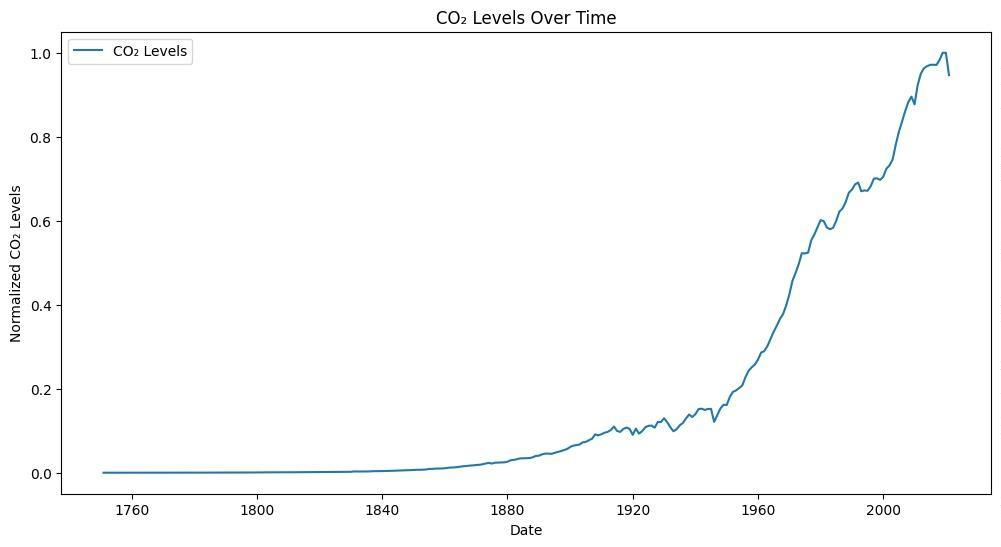
\includegraphics[width=457.9pt,height=250.23pt]{latexImage_d2063e50549ed4418c57a5f93d8925e6.png}}
\end{picture}
\newpage
\begin{tikzpicture}[overlay]\path(0pt,0pt);\end{tikzpicture}
\begin{picture}(-5,0)(2.5,0)
\put(21.6,-35.35999){\fontsize{9.96}{1}\usefont{T1}{cmr}{m}{n}\selectfont\color{color_29791}  Breaking the Carbon Curve                                                                                                                                                  AY 2024-25 }
\end{picture}
\begin{tikzpicture}[overlay]
\path(0pt,0pt);
\filldraw[color_156561][even odd rule]
(20.16pt, -42.91998pt) -- (561.8199pt, -42.91998pt)
 -- (561.8199pt, -42.91998pt)
 -- (561.8199pt, -39.91998pt)
 -- (561.8199pt, -39.91998pt)
 -- (20.16pt, -39.91998pt) -- cycle
;
\filldraw[color_156561][even odd rule]
(20.16pt, -39.20001pt) -- (561.8199pt, -39.20001pt)
 -- (561.8199pt, -39.20001pt)
 -- (561.8199pt, -38.48004pt)
 -- (561.8199pt, -38.48004pt)
 -- (20.16pt, -38.48004pt) -- cycle
;
\end{tikzpicture}
\begin{picture}(-5,0)(2.5,0)
\put(291.05,-53.47998){\fontsize{11.04}{1}\usefont{T1}{cmr}{m}{n}\selectfont\color{color_29791} }
\put(21.6,-743.96){\fontsize{9.96}{1}\usefont{T1}{cmr}{m}{n}\selectfont\color{color_29791}     Dept. of CSE, DSCE                                                                                                                                                                          9 }
\end{picture}
\begin{tikzpicture}[overlay]
\path(0pt,0pt);
\filldraw[color_156561][even odd rule]
(20.16pt, -732.176pt) -- (568.92pt, -732.176pt)
 -- (568.92pt, -732.176pt)
 -- (568.92pt, -729.176pt)
 -- (568.92pt, -729.176pt)
 -- (20.16pt, -729.176pt) -- cycle
;
\filldraw[color_156561][even odd rule]
(20.16pt, -733.616pt) -- (568.92pt, -733.616pt)
 -- (568.92pt, -733.616pt)
 -- (568.92pt, -732.896pt)
 -- (568.92pt, -732.896pt)
 -- (20.16pt, -732.896pt) -- cycle
;
\end{tikzpicture}
\begin{picture}(-5,0)(2.5,0)
\put(57.024,-73.17999){\fontsize{12}{1}\usefont{T1}{cmr}{m}{n}\selectfont\color{color_29791}same time, the project takes a dual approach—embracing innovation with hybrid models while }
\put(57.024,-93.82001){\fontsize{12}{1}\usefont{T1}{cmr}{m}{n}\selectfont\color{color_29791}validating their performance against established techniques to ensure reliability and }
\put(57.024,-114.58){\fontsize{12}{1}\usefont{T1}{cmr}{m}{n}\selectfont\color{color_29791}trustworthiness. }
\put(57.024,-143.26){\fontsize{12}{1}\usefont{T1}{cmr}{m}{n}\selectfont\color{color_29791} Beyond large-scale forecasting, the project also focuses on empowering individuals to }
\put(57.024,-164.02){\fontsize{12}{1}\usefont{T1}{cmr}{m}{n}\selectfont\color{color_29791}take action. It introduces an AI-powered personal CO2 assistant that helps users estimate their }
\put(57.024,-184.66){\fontsize{12}{1}\usefont{T1}{cmr}{m}{n}\selectfont\color{color_29791}carbon footprints and provides practical recommendations for reducing emissions. This tool }
\put(57.024,-205.42){\fontsize{12}{1}\usefont{T1}{cmr}{m}{n}\selectfont\color{color_29791}bridges the gap between the big picture of global emissions trends and the small but vital actions }
\put(57.024,-226.06){\fontsize{12}{1}\usefont{T1}{cmr}{m}{n}\selectfont\color{color_29791}individuals can take to contribute to climate goals. }
\put(57.024,-254.77){\fontsize{12}{1}\usefont{T1}{cmr}{m}{n}\selectfont\color{color_29791} Key challenges include managing the complexity and variability of time-series data, }
\put(57.024,-275.53){\fontsize{12}{1}\usefont{T1}{cmr}{m}{n}\selectfont\color{color_29791}making the models interpretable, and designing a user-friendly interface for the assistant. To }
\put(57.024,-296.17){\fontsize{12}{1}\usefont{T1}{cmr}{m}{n}\selectfont\color{color_29791}address these, the project uses hybrid model technique to provide insights into how the models }
\put(57.024,-316.93){\fontsize{12}{1}\usefont{T1}{cmr}{m}{n}\selectfont\color{color_29791}make predictions and employs advanced data pre-processing methods to clean and normalize noisy }
\put(57.024,-337.57){\fontsize{12}{1}\usefont{T1}{cmr}{m}{n}\selectfont\color{color_29791}datasets. }
\put(57.024,-366.25){\fontsize{12}{1}\usefont{T1}{cmr}{m}{n}\selectfont\color{color_29791} The project is built on a modular system design that breaks down tasks into manageable }
\put(57.024,-387.01){\fontsize{12}{1}\usefont{T1}{cmr}{m}{n}\selectfont\color{color_29791}stages: data cleaning, model training, evaluation, and deployment. This approach ensures a smooth }
\put(57.024,-407.67){\fontsize{12}{1}\usefont{T1}{cmr}{m}{n}\selectfont\color{color_29791}workflow and allows for future enhancements, making the system adaptable and scalable. By }
\put(57.024,-428.43){\fontsize{12}{1}\usefont{T1}{cmr}{m}{n}\selectfont\color{color_29791}balancing technical innovation with user-friendly design, the project aims to deliver meaningful }
\put(57.024,-449.07){\fontsize{12}{1}\usefont{T1}{cmr}{m}{n}\selectfont\color{color_29791}outcomes for policymakers, organizations, and individuals alike, contributing to a more }
\put(57.024,-469.83){\fontsize{12}{1}\usefont{T1}{cmr}{m}{n}\selectfont\color{color_29791}sustainable future for all. }
\put(57.024,-498.51){\fontsize{12}{1}\usefont{T1}{cmr}{m}{n}\selectfont\color{color_29791} }
\put(57.024,-531.03){\fontsize{15.96}{1}\usefont{T1}{cmr}{m}{n}\selectfont\color{color_29791}3.2 Hardware Requirements }
\put(75.024,-562.83){\fontsize{12}{1}\usefont{T1}{cmr}{m}{n}\selectfont\color{color_29791}1. High-performance CPU (e.g., Intel i7 or higher) for data preprocessing. }
\put(75.024,-591.54){\fontsize{12}{1}\usefont{T1}{cmr}{m}{n}\selectfont\color{color_29791}2. GPU (e.g., NVIDIA RTX 3060 or higher) for training deep learning models. }
\put(75.024,-620.22){\fontsize{12}{1}\usefont{T1}{cmr}{m}{n}\selectfont\color{color_29791}3. Minimum 16GB RAM for handling large datasets. }
\put(75.024,-648.9){\fontsize{12}{1}\usefont{T1}{cmr}{m}{n}\selectfont\color{color_29791}4. 1TB SSD for faster storage and retrieval of data and models. }
\put(75.024,-677.58){\fontsize{12}{1}\usefont{T1}{cmr}{m}{n}\selectfont\color{color_29791}5. Internet connectivity for cloud-based tools and dataset access. }
\put(57.024,-706.256){\fontsize{12}{1}\usefont{T1}{cmr}{m}{n}\selectfont\color{color_29791} }
\end{picture}
\newpage
\begin{tikzpicture}[overlay]\path(0pt,0pt);\end{tikzpicture}
\begin{picture}(-5,0)(2.5,0)
\put(21.6,-35.35999){\fontsize{9.96}{1}\usefont{T1}{cmr}{m}{n}\selectfont\color{color_29791}  Breaking the Carbon Curve                                                                                                                                                  AY 2024-25 }
\end{picture}
\begin{tikzpicture}[overlay]
\path(0pt,0pt);
\filldraw[color_156561][even odd rule]
(20.16pt, -42.91998pt) -- (561.8199pt, -42.91998pt)
 -- (561.8199pt, -42.91998pt)
 -- (561.8199pt, -39.91998pt)
 -- (561.8199pt, -39.91998pt)
 -- (20.16pt, -39.91998pt) -- cycle
;
\filldraw[color_156561][even odd rule]
(20.16pt, -39.20001pt) -- (561.8199pt, -39.20001pt)
 -- (561.8199pt, -39.20001pt)
 -- (561.8199pt, -38.48004pt)
 -- (561.8199pt, -38.48004pt)
 -- (20.16pt, -38.48004pt) -- cycle
;
\end{tikzpicture}
\begin{picture}(-5,0)(2.5,0)
\put(291.05,-53.47998){\fontsize{11.04}{1}\usefont{T1}{cmr}{m}{n}\selectfont\color{color_29791} }
\put(21.6,-743.96){\fontsize{9.96}{1}\usefont{T1}{cmr}{m}{n}\selectfont\color{color_29791}     Dept. of CSE, DSCE                                                                                                                                                                          10 }
\end{picture}
\begin{tikzpicture}[overlay]
\path(0pt,0pt);
\filldraw[color_156561][even odd rule]
(20.16pt, -732.176pt) -- (568.92pt, -732.176pt)
 -- (568.92pt, -732.176pt)
 -- (568.92pt, -729.176pt)
 -- (568.92pt, -729.176pt)
 -- (20.16pt, -729.176pt) -- cycle
;
\filldraw[color_156561][even odd rule]
(20.16pt, -733.616pt) -- (568.92pt, -733.616pt)
 -- (568.92pt, -733.616pt)
 -- (568.92pt, -732.896pt)
 -- (568.92pt, -732.896pt)
 -- (20.16pt, -732.896pt) -- cycle
;
\end{tikzpicture}
\begin{picture}(-5,0)(2.5,0)
\put(57.024,-77.02002){\fontsize{15.96}{1}\usefont{T1}{cmr}{m}{n}\selectfont\color{color_29791}3.3 Software Requirements }
\put(75.024,-108.82){\fontsize{12}{1}\usefont{T1}{cmr}{m}{n}\selectfont\color{color_29791}1. Python 3.x for data analysis and model development. }
\put(75.024,-137.5){\fontsize{12}{1}\usefont{T1}{cmr}{m}{n}\selectfont\color{color_29791}2. Tensorflow for deep learning model implementation. }
\put(75.024,-166.18){\fontsize{12}{1}\usefont{T1}{cmr}{m}{n}\selectfont\color{color_29791}3. Power BI for creating data visualizations and dashboards. }
\put(75.024,-194.86){\fontsize{12}{1}\usefont{T1}{cmr}{m}{n}\selectfont\color{color_29791}4. Jupyter Notebook or Google Collab for exploratory data analysis (EDA). }
\put(75.024,-223.54){\fontsize{12}{1}\usefont{T1}{cmr}{m}{n}\selectfont\color{color_29791}5. Git/GitHub for version control and collaboration. }
\put(75.024,-252.25){\fontsize{12}{1}\usefont{T1}{cmr}{m}{n}\selectfont\color{color_29791}6. Retrieval Augmented Generation (RAG) software architecture for building AI-powered }
\put(93.02,-273.01){\fontsize{12}{1}\usefont{T1}{cmr}{m}{n}\selectfont\color{color_29791}personal CO2 assistant. }
\put(57.024,-301.69){\fontsize{12}{1}\usefont{T1}{cmr}{m}{n}\selectfont\color{color_29791}Libraries: pandas, NumPy, matplotlib, seaborn, scikit-learn }
\put(57.024,-334.21){\fontsize{15.96}{1}\usefont{T1}{cmr}{m}{n}\selectfont\color{color_29791} }
\put(57.024,-371.65){\fontsize{18}{1}\usefont{T1}{cmr}{m}{n}\selectfont\color{color_29791}3.4 System Architecture Design }
\put(57.024,-405.03){\fontsize{12}{1}\usefont{T1}{cmr}{m}{n}\selectfont\color{color_29791}The system architecture consists of the following components: }
\put(75.024,-433.71){\fontsize{12}{1}\usefont{T1}{cmr}{m}{n}\selectfont\color{color_29791}1. Data Layer: Handles data storage and preprocessing. }
\put(75.024,-462.51){\fontsize{12}{1}\usefont{T1}{cmr}{m}{n}\selectfont\color{color_29791}2. Modelling Layer: Includes ARIMA, CNN-GRU, and CNN-LSTM models for forecasting. }
\put(75.024,-491.19){\fontsize{12}{1}\usefont{T1}{cmr}{m}{n}\selectfont\color{color_29791}3. Application Layer: Supports the AI-powered personal CO2 assistant. }
\put(75.024,-519.87){\fontsize{12}{1}\usefont{T1}{cmr}{m}{n}\selectfont\color{color_29791}4. Visualization Layer: Provides insights through Power BI dashboards. }
\put(57.024,-554.19){\fontsize{18}{1}\usefont{T1}{cmr}{m}{n}\selectfont\color{color_29791} }
\put(57.024,-593.22){\fontsize{18}{1}\usefont{T1}{cmr}{m}{n}\selectfont\color{color_29791}3.5 Data Flow Diagram (DFD) }
\put(57.024,-626.7){\fontsize{12}{1}\usefont{T1}{cmr}{m}{n}\selectfont\color{color_29791}The DFD captures the flow of data through the system, from raw data ingestion to forecast outputs }
\put(57.024,-647.34){\fontsize{12}{1}\usefont{T1}{cmr}{m}{n}\selectfont\color{color_29791}and user recommendations. }
\put(57.024,-676.02){\fontsize{12}{1}\usefont{T1}{cmr}{m}{n}\selectfont\color{color_29791} }
\put(57.024,-704.816){\fontsize{12}{1}\usefont{T1}{cmr}{m}{n}\selectfont\color{color_29791} }
\end{picture}
\newpage
\begin{tikzpicture}[overlay]\path(0pt,0pt);\end{tikzpicture}
\begin{picture}(-5,0)(2.5,0)
\put(21.6,-35.35999){\fontsize{9.96}{1}\usefont{T1}{cmr}{m}{n}\selectfont\color{color_29791}  Breaking the Carbon Curve                                                                                                                                                  AY 2024-25 }
\end{picture}
\begin{tikzpicture}[overlay]
\path(0pt,0pt);
\filldraw[color_156561][even odd rule]
(20.16pt, -42.91998pt) -- (561.8199pt, -42.91998pt)
 -- (561.8199pt, -42.91998pt)
 -- (561.8199pt, -39.91998pt)
 -- (561.8199pt, -39.91998pt)
 -- (20.16pt, -39.91998pt) -- cycle
;
\filldraw[color_156561][even odd rule]
(20.16pt, -39.20001pt) -- (561.8199pt, -39.20001pt)
 -- (561.8199pt, -39.20001pt)
 -- (561.8199pt, -38.48004pt)
 -- (561.8199pt, -38.48004pt)
 -- (20.16pt, -38.48004pt) -- cycle
;
\end{tikzpicture}
\begin{picture}(-5,0)(2.5,0)
\put(291.05,-53.47998){\fontsize{11.04}{1}\usefont{T1}{cmr}{m}{n}\selectfont\color{color_29791} }
\put(21.6,-743.96){\fontsize{9.96}{1}\usefont{T1}{cmr}{m}{n}\selectfont\color{color_29791}     Dept. of CSE, DSCE                                                                                                                                                                          11 }
\end{picture}
\begin{tikzpicture}[overlay]
\path(0pt,0pt);
\filldraw[color_156561][even odd rule]
(20.16pt, -732.176pt) -- (568.92pt, -732.176pt)
 -- (568.92pt, -732.176pt)
 -- (568.92pt, -729.176pt)
 -- (568.92pt, -729.176pt)
 -- (20.16pt, -729.176pt) -- cycle
;
\filldraw[color_156561][even odd rule]
(20.16pt, -733.616pt) -- (568.92pt, -733.616pt)
 -- (568.92pt, -733.616pt)
 -- (568.92pt, -732.896pt)
 -- (568.92pt, -732.896pt)
 -- (20.16pt, -732.896pt) -- cycle
;
\end{tikzpicture}
\begin{picture}(-5,0)(2.5,0)
\put(57.024,-73.17999){\fontsize{12}{1}\usefont{T1}{cmr}{m}{n}\selectfont\color{color_29791} }
\put(57.024,-101.86){\fontsize{12}{1}\usefont{T1}{cmr}{m}{n}\selectfont\color{color_29791} }
\put(418.51,-433.23){\fontsize{12}{1}\usefont{T1}{cmr}{m}{n}\selectfont\color{color_29791} }
\put(291.05,-458.43){\fontsize{12}{1}\usefont{T1}{cmr}{m}{n}\selectfont\color{color_29791} }
\put(173.06,-486.27){\fontsize{12}{1}\usefont{T1}{cmr}{m}{n}\selectfont\color{color_29791}Figure 3.2: Data flow diagram of CO2 prediction }
\put(291.05,-520.95){\fontsize{12}{1}\usefont{T1}{cmr}{m}{n}\selectfont\color{color_29791} }
\put(57.024,-552.63){\fontsize{15.96}{1}\usefont{T1}{cmr}{m}{n}\selectfont\color{color_29791}3.6 Use Case Diagram }
\put(57.024,-584.46){\fontsize{12}{1}\usefont{T1}{cmr}{m}{n}\selectfont\color{color_29791}The use case diagram represents the interaction of the system with external users, including }
\put(57.024,-605.1){\fontsize{12}{1}\usefont{T1}{cmr}{m}{n}\selectfont\color{color_29791}policymakers, businesses, and individual users, highlighting the forecasting and assistant }
\put(57.024,-625.74){\fontsize{12}{1}\usefont{T1}{cmr}{m}{n}\selectfont\color{color_29791}func}
\put(163.5,-433.2501){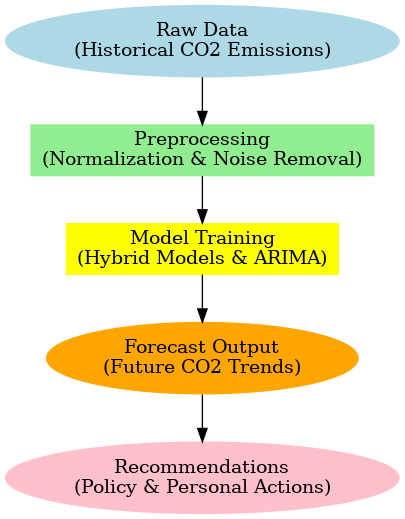
\includegraphics[width=254.9pt,height=307.85pt]{latexImage_7fc14597220026ce1ababc0106d7d444.png}}
\end{picture}
\newpage
\begin{tikzpicture}[overlay]\path(0pt,0pt);\end{tikzpicture}
\begin{picture}(-5,0)(2.5,0)
\put(21.6,-35.35999){\fontsize{9.96}{1}\usefont{T1}{cmr}{m}{n}\selectfont\color{color_29791}  Breaking the Carbon Curve                                                                                                                                                  AY 2024-25 }
\end{picture}
\begin{tikzpicture}[overlay]
\path(0pt,0pt);
\filldraw[color_156561][even odd rule]
(20.16pt, -42.91998pt) -- (561.8199pt, -42.91998pt)
 -- (561.8199pt, -42.91998pt)
 -- (561.8199pt, -39.91998pt)
 -- (561.8199pt, -39.91998pt)
 -- (20.16pt, -39.91998pt) -- cycle
;
\filldraw[color_156561][even odd rule]
(20.16pt, -39.20001pt) -- (561.8199pt, -39.20001pt)
 -- (561.8199pt, -39.20001pt)
 -- (561.8199pt, -38.48004pt)
 -- (561.8199pt, -38.48004pt)
 -- (20.16pt, -38.48004pt) -- cycle
;
\end{tikzpicture}
\begin{picture}(-5,0)(2.5,0)
\put(291.05,-53.47998){\fontsize{11.04}{1}\usefont{T1}{cmr}{m}{n}\selectfont\color{color_29791} }
\put(21.6,-743.96){\fontsize{9.96}{1}\usefont{T1}{cmr}{m}{n}\selectfont\color{color_29791}     Dept. of CSE, DSCE                                                                                                                                                                          12 }
\end{picture}
\begin{tikzpicture}[overlay]
\path(0pt,0pt);
\filldraw[color_156561][even odd rule]
(20.16pt, -732.176pt) -- (568.92pt, -732.176pt)
 -- (568.92pt, -732.176pt)
 -- (568.92pt, -729.176pt)
 -- (568.92pt, -729.176pt)
 -- (20.16pt, -729.176pt) -- cycle
;
\filldraw[color_156561][even odd rule]
(20.16pt, -733.616pt) -- (568.92pt, -733.616pt)
 -- (568.92pt, -733.616pt)
 -- (568.92pt, -732.896pt)
 -- (568.92pt, -732.896pt)
 -- (20.16pt, -732.896pt) -- cycle
;
\end{tikzpicture}
\begin{picture}(-5,0)(2.5,0)
\put(444.82,-363.73){\fontsize{12}{1}\usefont{T1}{cmr}{m}{n}\selectfont\color{color_29791} }
\put(168.86,-389.53){\fontsize{12}{1}\usefont{T1}{cmr}{m}{n}\selectfont\color{color_29791}Figure 3.6: Use case diagram of Prediction of CO2 }
\put(57.024,-423.99){\fontsize{18}{1}\usefont{T1}{cmr}{m}{n}\selectfont\color{color_29791} }
\put(57.024,-463.11){\fontsize{18}{1}\usefont{T1}{cmr}{m}{n}\selectfont\color{color_29791} }
\put(137.25,-363.65){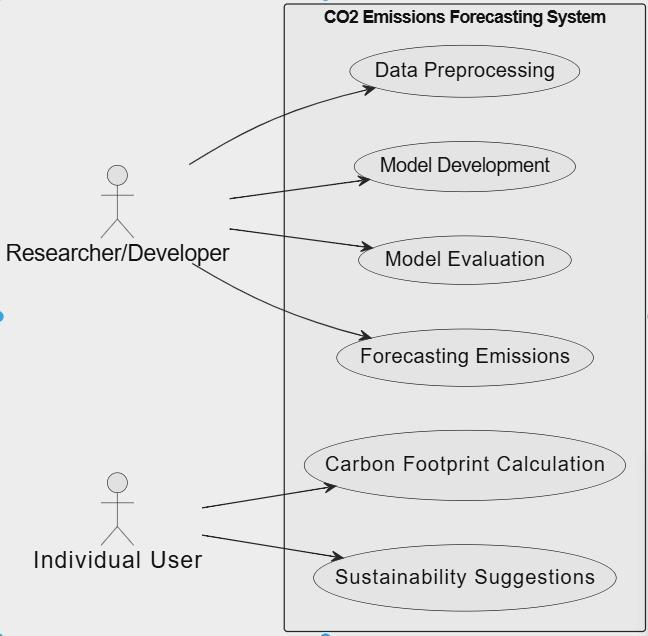
\includegraphics[width=307.33pt,height=301.65pt]{latexImage_6e648d6a6bf04bb3fcae8b625560c6f1.png}}
\end{picture}
\newpage
\begin{tikzpicture}[overlay]\path(0pt,0pt);\end{tikzpicture}
\begin{picture}(-5,0)(2.5,0)
\put(21.6,-35.35999){\fontsize{9.96}{1}\usefont{T1}{cmr}{m}{n}\selectfont\color{color_29791}  Breaking the Carbon Curve                                                                                                                                                  AY 2024-25 }
\end{picture}
\begin{tikzpicture}[overlay]
\path(0pt,0pt);
\filldraw[color_156561][even odd rule]
(20.16pt, -42.91998pt) -- (561.8199pt, -42.91998pt)
 -- (561.8199pt, -42.91998pt)
 -- (561.8199pt, -39.91998pt)
 -- (561.8199pt, -39.91998pt)
 -- (20.16pt, -39.91998pt) -- cycle
;
\filldraw[color_156561][even odd rule]
(20.16pt, -39.20001pt) -- (561.8199pt, -39.20001pt)
 -- (561.8199pt, -39.20001pt)
 -- (561.8199pt, -38.48004pt)
 -- (561.8199pt, -38.48004pt)
 -- (20.16pt, -38.48004pt) -- cycle
;
\end{tikzpicture}
\begin{picture}(-5,0)(2.5,0)
\put(291.05,-53.47998){\fontsize{11.04}{1}\usefont{T1}{cmr}{m}{n}\selectfont\color{color_29791} }
\put(21.6,-743.96){\fontsize{9.96}{1}\usefont{T1}{cmr}{m}{n}\selectfont\color{color_29791}     Dept. of CSE, DSCE                                                                                                                                                                          13 }
\end{picture}
\begin{tikzpicture}[overlay]
\path(0pt,0pt);
\filldraw[color_156561][even odd rule]
(20.16pt, -732.176pt) -- (568.92pt, -732.176pt)
 -- (568.92pt, -732.176pt)
 -- (568.92pt, -729.176pt)
 -- (568.92pt, -729.176pt)
 -- (20.16pt, -729.176pt) -- cycle
;
\filldraw[color_156561][even odd rule]
(20.16pt, -733.616pt) -- (568.92pt, -733.616pt)
 -- (568.92pt, -733.616pt)
 -- (568.92pt, -732.896pt)
 -- (568.92pt, -732.896pt)
 -- (20.16pt, -732.896pt) -- cycle
;
\end{tikzpicture}
\begin{picture}(-5,0)(2.5,0)
\put(57.024,-77.02002){\fontsize{15.96}{1}\usefont{T1}{cmr}{m}{n}\selectfont\color{color_29791}3.7 Sequence Diagram }
\put(57.024,-108.82){\fontsize{12}{1}\usefont{T1}{cmr}{m}{n}\selectfont\color{color_29791}The sequence diagram illustrates the interaction flow between system components, showcasing }
\put(57.024,-129.46){\fontsize{12}{1}\usefont{T1}{cmr}{m}{n}\selectfont\color{color_29791}the end-to-end process from data input to actionable insights. }
\put(525.1,-507.03){\fontsize{12}{1}\usefont{T1}{cmr}{m}{n}\selectfont\color{color_29791} }
\put(146.66,-532.95){\fontsize{12}{1}\usefont{T1}{cmr}{m}{n}\selectfont\color{color_29791}Figure 3.7: Sequence diagram for CO2 emissions prediction }
\put(57.024,-567.27){\fontsize{18}{1}\usefont{T1}{cmr}{m}{n}\selectfont\color{color_29791} }
\put(57.024,-606.3){\fontsize{18}{1}\usefont{T1}{cmr}{m}{n}\selectfont\color{color_29791} }
\put(57.024,-645.42){\fontsize{18}{1}\usefont{T1}{cmr}{m}{n}\selectfont\color{color_29791} }
\put(57.024,-684.416){\fontsize{18}{1}\usefont{T1}{cmr}{m}{n}\selectfont\color{color_29791} }
\put(57,-506.49){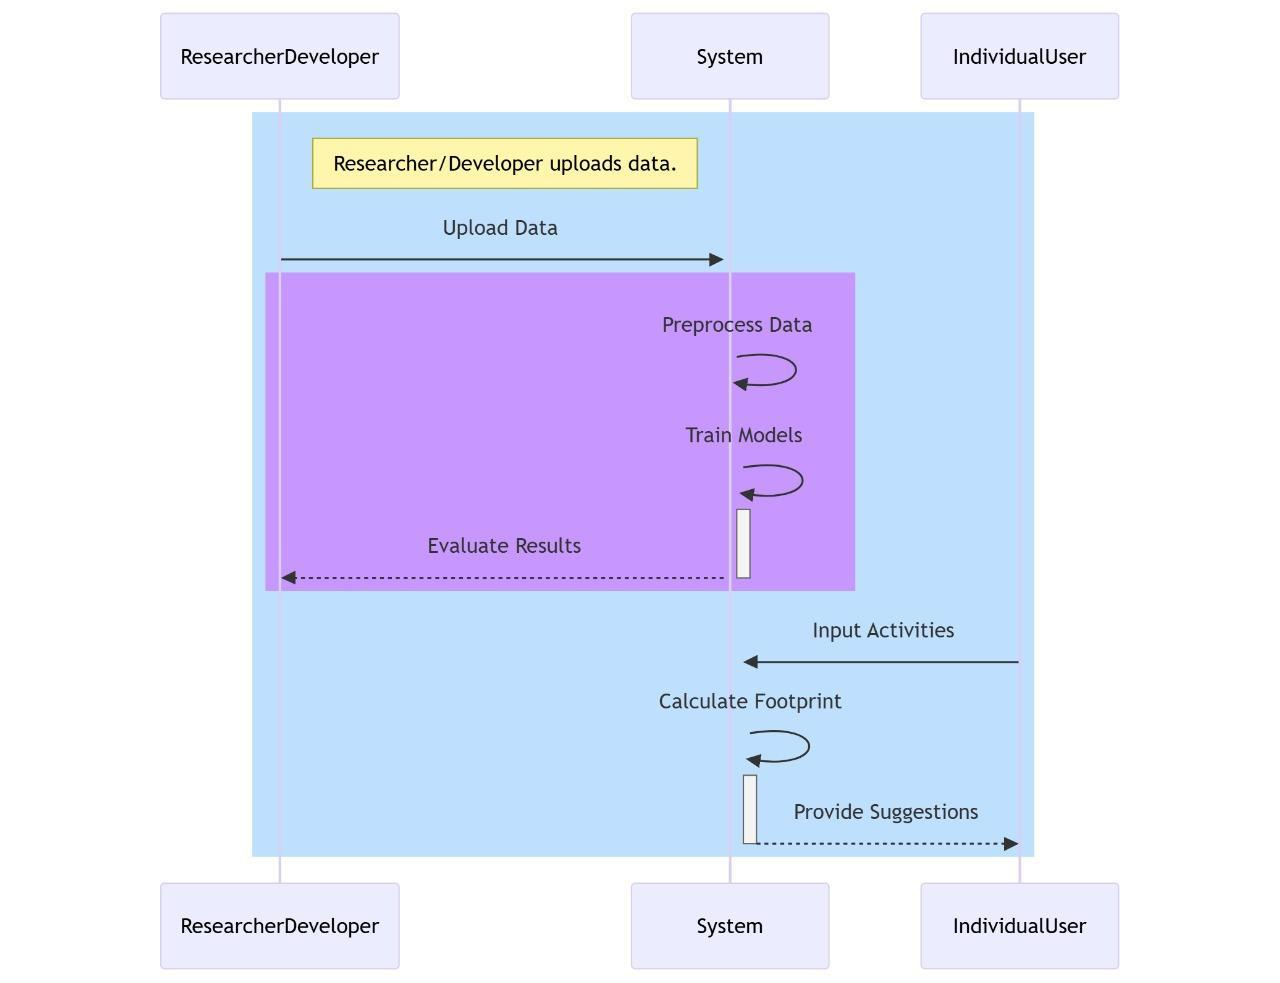
\includegraphics[width=468pt,height=359.5pt]{latexImage_e20f1b46115aea0cae6d5e7c13afef88.png}}
\end{picture}
\newpage
\begin{tikzpicture}[overlay]\path(0pt,0pt);\end{tikzpicture}
\begin{picture}(-5,0)(2.5,0)
\put(21.6,-35.35999){\fontsize{9.96}{1}\usefont{T1}{cmr}{m}{n}\selectfont\color{color_29791}  Breaking the Carbon Curve                                                                                                                                                  AY 2024-25 }
\end{picture}
\begin{tikzpicture}[overlay]
\path(0pt,0pt);
\filldraw[color_156561][even odd rule]
(20.16pt, -42.91998pt) -- (561.8199pt, -42.91998pt)
 -- (561.8199pt, -42.91998pt)
 -- (561.8199pt, -39.91998pt)
 -- (561.8199pt, -39.91998pt)
 -- (20.16pt, -39.91998pt) -- cycle
;
\filldraw[color_156561][even odd rule]
(20.16pt, -39.20001pt) -- (561.8199pt, -39.20001pt)
 -- (561.8199pt, -39.20001pt)
 -- (561.8199pt, -38.48004pt)
 -- (561.8199pt, -38.48004pt)
 -- (20.16pt, -38.48004pt) -- cycle
;
\end{tikzpicture}
\begin{picture}(-5,0)(2.5,0)
\put(291.05,-53.47998){\fontsize{11.04}{1}\usefont{T1}{cmr}{m}{n}\selectfont\color{color_29791} }
\put(21.6,-743.96){\fontsize{9.96}{1}\usefont{T1}{cmr}{m}{n}\selectfont\color{color_29791}     Dept. of CSE, DSCE                                                                                                                                                                          14 }
\end{picture}
\begin{tikzpicture}[overlay]
\path(0pt,0pt);
\filldraw[color_156561][even odd rule]
(20.16pt, -732.176pt) -- (568.92pt, -732.176pt)
 -- (568.92pt, -732.176pt)
 -- (568.92pt, -729.176pt)
 -- (568.92pt, -729.176pt)
 -- (20.16pt, -729.176pt) -- cycle
;
\filldraw[color_156561][even odd rule]
(20.16pt, -733.616pt) -- (568.92pt, -733.616pt)
 -- (568.92pt, -733.616pt)
 -- (568.92pt, -732.896pt)
 -- (568.92pt, -732.896pt)
 -- (20.16pt, -732.896pt) -- cycle
;
\end{tikzpicture}
\begin{picture}(-5,0)(2.5,0)
\put(57.024,-80.73999){\fontsize{20.04}{1}\usefont{T1}{cmr}{m}{n}\selectfont\color{color_29791}Chapter 4 }
\put(240.05,-111.7){\fontsize{18}{1}\usefont{T1}{cmr}{m}{n}\selectfont\color{color_29791}Implementation }
\put(57.024,-141.94){\fontsize{18}{1}\usefont{T1}{cmr}{m}{n}\selectfont\color{color_29791} }
\put(57.024,-179.26){\fontsize{15.96}{1}\usefont{T1}{cmr}{m}{n}\selectfont\color{color_29791}4.1 Overview of System Implementation }
\put(57.024,-210.94){\fontsize{12}{1}\usefont{T1}{cmr}{m}{n}\selectfont\color{color_29791}The implementation of the CO2 emissions forecasting system focuses on blending advanced data-}
\put(57.024,-231.7){\fontsize{12}{1}\usefont{T1}{cmr}{m}{n}\selectfont\color{color_29791}driven techniques with hybrid machine learning models to produce meaningful and actionable }
\put(57.024,-252.37){\fontsize{12}{1}\usefont{T1}{cmr}{m}{n}\selectfont\color{color_29791}insights. It all begins with a rigorous pre-processing phase where the dataset is carefully cleaned, }
\put(57.024,-273.13){\fontsize{12}{1}\usefont{T1}{cmr}{m}{n}\selectfont\color{color_29791}normalized, and enriched with useful features like cumulative emissions, yearly growth rates, and }
\put(57.024,-293.77){\fontsize{12}{1}\usefont{T1}{cmr}{m}{n}\selectfont\color{color_29791}sector-wise contributions. These steps ensure that the data is ready for the sophisticated models to }
\put(57.024,-314.53){\fontsize{12}{1}\usefont{T1}{cmr}{m}{n}\selectfont\color{color_29791}extract the insights we need. }
\put(57.024,-343.21){\fontsize{12}{1}\usefont{T1}{cmr}{m}{n}\selectfont\color{color_29791} The forecasting process leverages hybrid deep learning models, such as CNN-GRU and }
\put(57.024,-363.85){\fontsize{12}{1}\usefont{T1}{cmr}{m}{n}\selectfont\color{color_29791}CNN-LSTM, which combine the strengths of Convolutional Neural Networks (CNNs) for }
\put(57.024,-384.61){\fontsize{12}{1}\usefont{T1}{cmr}{m}{n}\selectfont\color{color_29791}identifying patterns and temporal models like GRU and LSTM for analysing time-based trends. }
\put(57.024,-405.27){\fontsize{12}{1}\usefont{T1}{cmr}{m}{n}\selectfont\color{color_29791}These advanced architectures are benchmarked against traditional methods like ARIMA and }
\put(57.024,-426.03){\fontsize{12}{1}\usefont{T1}{cmr}{m}{n}\selectfont\color{color_29791}standalone LSTM models to evaluate their effectiveness in dealing with complex time-series data. }
\put(57.024,-446.67){\fontsize{12}{1}\usefont{T1}{cmr}{m}{n}\selectfont\color{color_29791}The models are trained and validated on carefully split datasets, ensuring they are both robust and }
\put(57.024,-467.43){\fontsize{12}{1}\usefont{T1}{cmr}{m}{n}\selectfont\color{color_29791}scalable. }
\put(57.024,-496.11){\fontsize{12}{1}\usefont{T1}{cmr}{m}{n}\selectfont\color{color_29791} A key focus of the implementation is transparency, the system offers insights into which }
\put(57.024,-516.75){\fontsize{12}{1}\usefont{T1}{cmr}{m}{n}\selectfont\color{color_29791}features influence the models' predictions the most. This helps users trust the results and }
\put(57.024,-537.51){\fontsize{12}{1}\usefont{T1}{cmr}{m}{n}\selectfont\color{color_29791}understand the underlying patterns. To make the results accessible and actionable, Power BI }
\put(57.024,-558.15){\fontsize{12}{1}\usefont{T1}{cmr}{m}{n}\selectfont\color{color_29791}dashboards visualize trends, sectoral contributions, and country-level comparisons through }
\put(57.024,-578.94){\fontsize{12}{1}\usefont{T1}{cmr}{m}{n}\selectfont\color{color_29791}interactive tools. }
\put(57.024,-607.62){\fontsize{12}{1}\usefont{T1}{cmr}{m}{n}\selectfont\color{color_29791} Additionally, the project includes an AI-powered assistant, built on large language models }
\put(57.024,-628.38){\fontsize{12}{1}\usefont{T1}{cmr}{m}{n}\selectfont\color{color_29791}(LLMs), to help users calculate their carbon footprints and take meaningful steps to reduce them. }
\put(57.024,-649.02){\fontsize{12}{1}\usefont{T1}{cmr}{m}{n}\selectfont\color{color_29791}This tool brings the insights down to the individual level, enabling personal and organizational }
\put(57.024,-669.78){\fontsize{12}{1}\usefont{T1}{cmr}{m}{n}\selectfont\color{color_29791}contributions to global climate goals. }
\put(57.024,-698.456){\fontsize{12}{1}\usefont{T1}{cmr}{m}{n}\selectfont\color{color_29791} }
\end{picture}
\newpage
\begin{tikzpicture}[overlay]\path(0pt,0pt);\end{tikzpicture}
\begin{picture}(-5,0)(2.5,0)
\put(21.6,-35.35999){\fontsize{9.96}{1}\usefont{T1}{cmr}{m}{n}\selectfont\color{color_29791}  Breaking the Carbon Curve                                                                                                                                                  AY 2024-25 }
\end{picture}
\begin{tikzpicture}[overlay]
\path(0pt,0pt);
\filldraw[color_156561][even odd rule]
(20.16pt, -42.91998pt) -- (561.8199pt, -42.91998pt)
 -- (561.8199pt, -42.91998pt)
 -- (561.8199pt, -39.91998pt)
 -- (561.8199pt, -39.91998pt)
 -- (20.16pt, -39.91998pt) -- cycle
;
\filldraw[color_156561][even odd rule]
(20.16pt, -39.20001pt) -- (561.8199pt, -39.20001pt)
 -- (561.8199pt, -39.20001pt)
 -- (561.8199pt, -38.48004pt)
 -- (561.8199pt, -38.48004pt)
 -- (20.16pt, -38.48004pt) -- cycle
;
\end{tikzpicture}
\begin{picture}(-5,0)(2.5,0)
\put(291.05,-53.47998){\fontsize{11.04}{1}\usefont{T1}{cmr}{m}{n}\selectfont\color{color_29791} }
\put(21.6,-743.96){\fontsize{9.96}{1}\usefont{T1}{cmr}{m}{n}\selectfont\color{color_29791}     Dept. of CSE, DSCE                                                                                                                                                                          15 }
\end{picture}
\begin{tikzpicture}[overlay]
\path(0pt,0pt);
\filldraw[color_156561][even odd rule]
(20.16pt, -732.176pt) -- (568.92pt, -732.176pt)
 -- (568.92pt, -732.176pt)
 -- (568.92pt, -729.176pt)
 -- (568.92pt, -729.176pt)
 -- (20.16pt, -729.176pt) -- cycle
;
\filldraw[color_156561][even odd rule]
(20.16pt, -733.616pt) -- (568.92pt, -733.616pt)
 -- (568.92pt, -733.616pt)
 -- (568.92pt, -732.896pt)
 -- (568.92pt, -732.896pt)
 -- (20.16pt, -732.896pt) -- cycle
;
\end{tikzpicture}
\begin{picture}(-5,0)(2.5,0)
\put(57.024,-77.02002){\fontsize{15.96}{1}\usefont{T1}{cmr}{m}{n}\selectfont\color{color_29791}4.2 Model Description }
\put(57.024,-112.66){\fontsize{15.96}{1}\usefont{T1}{cmr}{m}{n}\selectfont\color{color_29791}4.2.1 Prediction using Models }
\put(57.024,-144.34){\fontsize{12}{1}\usefont{T1}{cmr}{m}{n}\selectfont\color{color_29791}1. Data Preprocessing Model }
\put(75.024,-173.02){\fontsize{9.96}{1}\usefont{T1}{cmr}{m}{n}\selectfont\color{color_29791}• Data Cleaning: Removes missing values, detects outliers, and ensures the dataset is }
\put(93.02,-193.78){\fontsize{12}{1}\usefont{T1}{cmr}{m}{n}\selectfont\color{color_29791}consistently formatted for analysis. }
\put(75.024,-222.46){\fontsize{9.96}{1}\usefont{T1}{cmr}{m}{n}\selectfont\color{color_29791}• Feature Engineering: Adds calculated features, such as cumulative emissions and yearly }
\put(93.02,-243.25){\fontsize{12}{1}\usefont{T1}{cmr}{m}{n}\selectfont\color{color_29791}growth rates, to enrich the data. }
\put(75.024,-271.93){\fontsize{9.96}{1}\usefont{T1}{cmr}{m}{n}\selectfont\color{color_29791}• Data Normalization: Scales the data to a uniform range, ensuring compatibility with the }
\put(93.02,-292.57){\fontsize{12}{1}\usefont{T1}{cmr}{m}{n}\selectfont\color{color_29791}deep learning models. }
\put(75.024,-321.25){\fontsize{9.96}{1}\usefont{T1}{cmr}{m}{n}\selectfont\color{color_29791}• Sequence Generation: Prepares overlapping time-series sequences, turning the raw data }
\put(93.02,-342.01){\fontsize{12}{1}\usefont{T1}{cmr}{m}{n}\selectfont\color{color_29791}into model-ready inputs. }
\put(57.024,-370.69){\fontsize{12}{1}\usefont{T1}{cmr}{m}{n}\selectfont\color{color_29791}2. Modelling Module }
\put(75.024,-399.37){\fontsize{9.96}{1}\usefont{T1}{cmr}{m}{n}\selectfont\color{color_29791}• CNN-GRU Model: Combines CNN layers for identifying patterns in data with GRU }
\put(93.02,-420.15){\fontsize{12}{1}\usefont{T1}{cmr}{m}{n}\selectfont\color{color_29791}layers for capturing trends over time. }
\put(75.024,-448.83){\fontsize{9.96}{1}\usefont{T1}{cmr}{m}{n}\selectfont\color{color_29791}• CNN-LSTM Model: Uses CNNs for spatial feature extraction and LSTM layers to analyse }
\put(93.02,-469.47){\fontsize{12}{1}\usefont{T1}{cmr}{m}{n}\selectfont\color{color_29791}long-term dependencies in the data. }
\put(75.024,-498.15){\fontsize{9.96}{1}\usefont{T1}{cmr}{m}{n}\selectfont\color{color_29791}• ARIMA and LSTM Baselines: Implements ARIMA as a statistical benchmark and }
\put(93.02,-518.91){\fontsize{12}{1}\usefont{T1}{cmr}{m}{n}\selectfont\color{color_29791}standalone LSTM as a deep learning comparison. }
\put(75.024,-547.59){\fontsize{9.96}{1}\usefont{T1}{cmr}{m}{n}\selectfont\color{color_29791}• Training and Validation: Splits the data into training, validation, and test sets, fine-tuning }
\put(93.02,-568.35){\fontsize{12}{1}\usefont{T1}{cmr}{m}{n}\selectfont\color{color_29791}models for optimal performance. }
\put(75.024,-597.06){\fontsize{9.96}{1}\usefont{T1}{cmr}{m}{n}\selectfont\color{color_29791}• Evaluation Metrics: Compares model accuracy using metrics like Mean Absolute Error }
\put(93.02,-617.7){\fontsize{12}{1}\usefont{T1}{cmr}{m}{n}\selectfont\color{color_29791}(MAE), Root Mean Squared Error (RMSE), and R² scores. }
\put(93.02,-646.38){\fontsize{12}{1}\usefont{T1}{cmr}{m}{n}\selectfont\color{color_29791} }
\put(93.02,-675.06){\fontsize{12}{1}\usefont{T1}{cmr}{m}{n}\selectfont\color{color_29791} }
\end{picture}
\newpage
\begin{tikzpicture}[overlay]\path(0pt,0pt);\end{tikzpicture}
\begin{picture}(-5,0)(2.5,0)
\put(21.6,-35.35999){\fontsize{9.96}{1}\usefont{T1}{cmr}{m}{n}\selectfont\color{color_29791}  Breaking the Carbon Curve                                                                                                                                                  AY 2024-25 }
\end{picture}
\begin{tikzpicture}[overlay]
\path(0pt,0pt);
\filldraw[color_156561][even odd rule]
(20.16pt, -42.91998pt) -- (561.8199pt, -42.91998pt)
 -- (561.8199pt, -42.91998pt)
 -- (561.8199pt, -39.91998pt)
 -- (561.8199pt, -39.91998pt)
 -- (20.16pt, -39.91998pt) -- cycle
;
\filldraw[color_156561][even odd rule]
(20.16pt, -39.20001pt) -- (561.8199pt, -39.20001pt)
 -- (561.8199pt, -39.20001pt)
 -- (561.8199pt, -38.48004pt)
 -- (561.8199pt, -38.48004pt)
 -- (20.16pt, -38.48004pt) -- cycle
;
\end{tikzpicture}
\begin{picture}(-5,0)(2.5,0)
\put(291.05,-53.47998){\fontsize{11.04}{1}\usefont{T1}{cmr}{m}{n}\selectfont\color{color_29791} }
\put(21.6,-743.96){\fontsize{9.96}{1}\usefont{T1}{cmr}{m}{n}\selectfont\color{color_29791}     Dept. of CSE, DSCE                                                                                                                                                                          16 }
\end{picture}
\begin{tikzpicture}[overlay]
\path(0pt,0pt);
\filldraw[color_156561][even odd rule]
(20.16pt, -732.176pt) -- (568.92pt, -732.176pt)
 -- (568.92pt, -732.176pt)
 -- (568.92pt, -729.176pt)
 -- (568.92pt, -729.176pt)
 -- (20.16pt, -729.176pt) -- cycle
;
\filldraw[color_156561][even odd rule]
(20.16pt, -733.616pt) -- (568.92pt, -733.616pt)
 -- (568.92pt, -733.616pt)
 -- (568.92pt, -732.896pt)
 -- (568.92pt, -732.896pt)
 -- (20.16pt, -732.896pt) -- cycle
;
\end{tikzpicture}
\begin{picture}(-5,0)(2.5,0)
\put(57.024,-77.02002){\fontsize{15.96}{1}\usefont{T1}{cmr}{m}{n}\selectfont\color{color_29791}4.3 Data Analysis and Visualization }
\put(57.024,-108.82){\fontsize{12}{1}\usefont{T1}{cmr}{m}{n}\selectfont\color{color_29791}This section focuses on analysing and visualizing global CO2 emissions data to uncover actionable }
\put(57.024,-129.46){\fontsize{12}{1}\usefont{T1}{cmr}{m}{n}\selectfont\color{color_29791}insights. These insights can help stakeholders design effective policies, promote sustainable }
\put(57.024,-150.22){\fontsize{12}{1}\usefont{T1}{cmr}{m}{n}\selectfont\color{color_29791}practices, and prioritize interventions at national and sectoral levels. }
\put(57.024,-178.9){\fontsize{12}{1}\usefont{T1}{cmr}{m}{n}\selectfont\color{color_29791} }
\put(57.024,-207.58){\fontsize{12}{1}\usefont{T1}{cmr}{m}{n}\selectfont\color{color_29791}4.3.1 Overview of the Dataset }
\put(57.024,-236.29){\fontsize{12}{1}\usefont{T1}{cmr}{m}{n}\selectfont\color{color_29791}The dataset spans from January 2019 to May 2023, covering CO2 emissions from 14 countries }
\put(57.024,-257.05){\fontsize{12}{1}\usefont{T1}{cmr}{m}{n}\selectfont\color{color_29791}and six sectors, with 1,612 unique timestamps and over 127,000 data points. With no missing or }
\put(57.024,-277.69){\fontsize{12}{1}\usefont{T1}{cmr}{m}{n}\selectfont\color{color_29791}null values, the data is reliable and provides a strong basis for in-depth analysis. Preprocessing was }
\put(57.024,-298.45){\fontsize{12}{1}\usefont{T1}{cmr}{m}{n}\selectfont\color{color_29791}conducted to generate additional calculated columns, enabling a more detailed exploration of }
\put(57.024,-319.09){\fontsize{12}{1}\usefont{T1}{cmr}{m}{n}\selectfont\color{color_29791}emission patterns. }
\put(57.024,-347.77){\fontsize{12}{1}\usefont{T1}{cmr}{m}{n}\selectfont\color{color_29791} }
\put(525.1,-628.26){\fontsize{12}{1}\usefont{T1}{cmr}{m}{n}\selectfont\color{color_29791} }
\put(172.34,-654.18){\fontsize{12}{1}\usefont{T1}{cmr}{m}{n}\selectfont\color{color_29791}Figure 4.3.1: Overview of CO2 emissions dataset }
\put(291.05,-682.856){\fontsize{12}{1}\usefont{T1}{cmr}{m}{n}\selectfont\color{color_29791} }
\put(57,-628.23){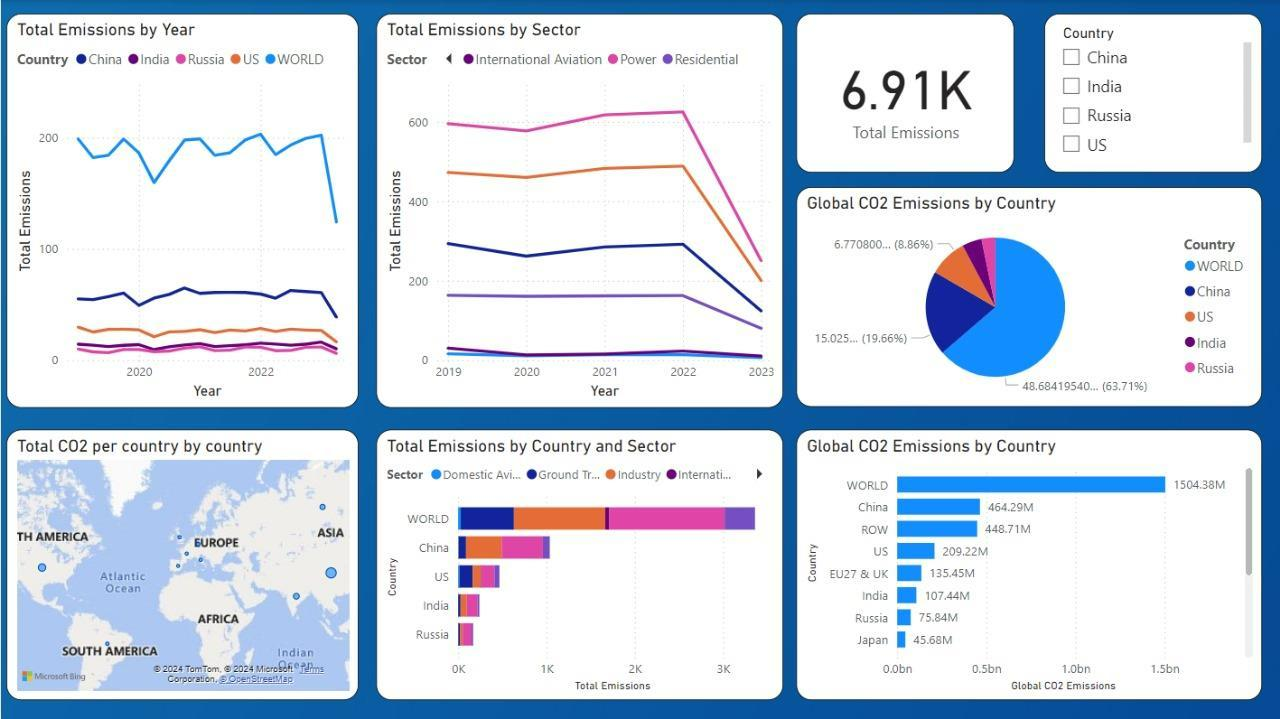
\includegraphics[width=468pt,height=262.95pt]{latexImage_8a5b637f687c6a662990222753037f7f.png}}
\end{picture}
\newpage
\begin{tikzpicture}[overlay]\path(0pt,0pt);\end{tikzpicture}
\begin{picture}(-5,0)(2.5,0)
\put(21.6,-35.35999){\fontsize{9.96}{1}\usefont{T1}{cmr}{m}{n}\selectfont\color{color_29791}  Breaking the Carbon Curve                                                                                                                                                  AY 2024-25 }
\end{picture}
\begin{tikzpicture}[overlay]
\path(0pt,0pt);
\filldraw[color_156561][even odd rule]
(20.16pt, -42.91998pt) -- (561.8199pt, -42.91998pt)
 -- (561.8199pt, -42.91998pt)
 -- (561.8199pt, -39.91998pt)
 -- (561.8199pt, -39.91998pt)
 -- (20.16pt, -39.91998pt) -- cycle
;
\filldraw[color_156561][even odd rule]
(20.16pt, -39.20001pt) -- (561.8199pt, -39.20001pt)
 -- (561.8199pt, -39.20001pt)
 -- (561.8199pt, -38.48004pt)
 -- (561.8199pt, -38.48004pt)
 -- (20.16pt, -38.48004pt) -- cycle
;
\end{tikzpicture}
\begin{picture}(-5,0)(2.5,0)
\put(291.05,-53.47998){\fontsize{11.04}{1}\usefont{T1}{cmr}{m}{n}\selectfont\color{color_29791} }
\put(21.6,-743.96){\fontsize{9.96}{1}\usefont{T1}{cmr}{m}{n}\selectfont\color{color_29791}     Dept. of CSE, DSCE                                                                                                                                                                          17 }
\end{picture}
\begin{tikzpicture}[overlay]
\path(0pt,0pt);
\filldraw[color_156561][even odd rule]
(20.16pt, -732.176pt) -- (568.92pt, -732.176pt)
 -- (568.92pt, -732.176pt)
 -- (568.92pt, -729.176pt)
 -- (568.92pt, -729.176pt)
 -- (20.16pt, -729.176pt) -- cycle
;
\filldraw[color_156561][even odd rule]
(20.16pt, -733.616pt) -- (568.92pt, -733.616pt)
 -- (568.92pt, -733.616pt)
 -- (568.92pt, -732.896pt)
 -- (568.92pt, -732.896pt)
 -- (20.16pt, -732.896pt) -- cycle
;
\end{tikzpicture}
\begin{picture}(-5,0)(2.5,0)
\put(57.024,-73.17999){\fontsize{12}{1}\usefont{T1}{cmr}{m}{n}\selectfont\color{color_29791}4.3.2 Preprocessing and Feature Engineering }
\put(57.024,-101.86){\fontsize{12}{1}\usefont{T1}{cmr}{m}{n}\selectfont\color{color_29791}Several calculated columns were added to enhance the analysis: }
\put(75.024,-130.54){\fontsize{12}{1}\usefont{T1}{cmr}{m}{n}\selectfont\color{color_29791}➢ Total CO2 per Country }
\put(75.024,-152.26){\fontsize{12}{1}\usefont{T1}{cmr}{m}{n}\selectfont\color{color_29791}• Definition: The sum of emissions from all sectors for each country on a specific date. }
\put(75.024,-173.74){\fontsize{12}{1}\usefont{T1}{cmr}{m}{n}\selectfont\color{color_29791}• Purpose: Highlights the total contribution of each country to global emissions. }
\put(57.024,-202.42){\fontsize{12}{1}\usefont{T1}{cmr}{m}{n}\selectfont\color{color_29791} }
\put(75.024,-231.1){\fontsize{12}{1}\usefont{T1}{cmr}{m}{n}\selectfont\color{color_29791}➢ Sector Percentage per Country }
\put(75.024,-252.73){\fontsize{12}{1}\usefont{T1}{cmr}{m}{n}\selectfont\color{color_29791}• Definition: The share of a sector's emissions as a percentage of a country's total emissions. }
\put(75.024,-274.33){\fontsize{12}{1}\usefont{T1}{cmr}{m}{n}\selectfont\color{color_29791}• Purpose: Identifies dominant sectors driving emissions in each country. }
\put(57.024,-302.89){\fontsize{12}{1}\usefont{T1}{cmr}{m}{n}\selectfont\color{color_29791} }
\put(75.024,-331.69){\fontsize{12}{1}\usefont{T1}{cmr}{m}{n}\selectfont\color{color_29791}➢ Yearly Growth Rate }
\put(75.024,-353.29){\fontsize{12}{1}\usefont{T1}{cmr}{m}{n}\selectfont\color{color_29791}• Definition: The annual percentage change in emissions for a country or sector. }
\put(75.024,-374.89){\fontsize{12}{1}\usefont{T1}{cmr}{m}{n}\selectfont\color{color_29791}• Purpose: Tracks trends and detects anomalies, such as rapid increases or declines in }
\put(93.02,-395.41){\fontsize{12}{1}\usefont{T1}{cmr}{m}{n}\selectfont\color{color_29791}emissions. }
\put(93.02,-416.19){\fontsize{12}{1}\usefont{T1}{cmr}{m}{n}\selectfont\color{color_29791} }
\put(75.024,-436.83){\fontsize{12}{1}\usefont{T1}{cmr}{m}{n}\selectfont\color{color_29791}➢ Cumulative CO2 per Sector }
\put(75.024,-458.55){\fontsize{12}{1}\usefont{T1}{cmr}{m}{n}\selectfont\color{color_29791}• Definition: Total emissions from each sector over time. }
\put(75.024,-480.03){\fontsize{12}{1}\usefont{T1}{cmr}{m}{n}\selectfont\color{color_29791}• Purpose: Shows the long-term contribution of sectors to global emissions. }
\put(57.024,-508.71){\fontsize{12}{1}\usefont{T1}{cmr}{m}{n}\selectfont\color{color_29791} }
\put(75.024,-537.39){\fontsize{12}{1}\usefont{T1}{cmr}{m}{n}\selectfont\color{color_29791}➢ Global CO2 Percentage per Country }
\put(75.024,-558.99){\fontsize{12}{1}\usefont{T1}{cmr}{m}{n}\selectfont\color{color_29791}• Definition: A country’s emissions as a percentage of the global total. }
\put(75.024,-580.62){\fontsize{12}{1}\usefont{T1}{cmr}{m}{n}\selectfont\color{color_29791}• Purpose: Identifies major contributors to global emissions and their relative impact. }
\put(57.024,-609.18){\fontsize{12}{1}\usefont{T1}{cmr}{m}{n}\selectfont\color{color_29791}4.3.3 Key Countries and Sectors }
\put(75.024,-637.98){\fontsize{12}{1}\usefont{T1}{cmr}{m}{n}\selectfont\color{color_29791}➢ Countries Analysed: }
\put(75.024,-659.58){\fontsize{12}{1}\usefont{T1}{cmr}{m}{n}\selectfont\color{color_29791}• China (19.66\%): The largest emitter, driven by industrial growth and energy demands. }
\put(75.024,-681.18){\fontsize{12}{1}\usefont{T1}{cmr}{m}{n}\selectfont\color{color_29791}• India (4.55\%): A rapidly growing economy with increasing emissions. }
\end{picture}
\newpage
\begin{tikzpicture}[overlay]\path(0pt,0pt);\end{tikzpicture}
\begin{picture}(-5,0)(2.5,0)
\put(21.6,-35.35999){\fontsize{9.96}{1}\usefont{T1}{cmr}{m}{n}\selectfont\color{color_29791}  Breaking the Carbon Curve                                                                                                                                                  AY 2024-25 }
\end{picture}
\begin{tikzpicture}[overlay]
\path(0pt,0pt);
\filldraw[color_156561][even odd rule]
(20.16pt, -42.91998pt) -- (561.8199pt, -42.91998pt)
 -- (561.8199pt, -42.91998pt)
 -- (561.8199pt, -39.91998pt)
 -- (561.8199pt, -39.91998pt)
 -- (20.16pt, -39.91998pt) -- cycle
;
\filldraw[color_156561][even odd rule]
(20.16pt, -39.20001pt) -- (561.8199pt, -39.20001pt)
 -- (561.8199pt, -39.20001pt)
 -- (561.8199pt, -38.48004pt)
 -- (561.8199pt, -38.48004pt)
 -- (20.16pt, -38.48004pt) -- cycle
;
\end{tikzpicture}
\begin{picture}(-5,0)(2.5,0)
\put(291.05,-53.47998){\fontsize{11.04}{1}\usefont{T1}{cmr}{m}{n}\selectfont\color{color_29791} }
\put(21.6,-743.96){\fontsize{9.96}{1}\usefont{T1}{cmr}{m}{n}\selectfont\color{color_29791}     Dept. of CSE, DSCE                                                                                                                                                                          18 }
\end{picture}
\begin{tikzpicture}[overlay]
\path(0pt,0pt);
\filldraw[color_156561][even odd rule]
(20.16pt, -732.176pt) -- (568.92pt, -732.176pt)
 -- (568.92pt, -732.176pt)
 -- (568.92pt, -729.176pt)
 -- (568.92pt, -729.176pt)
 -- (20.16pt, -729.176pt) -- cycle
;
\filldraw[color_156561][even odd rule]
(20.16pt, -733.616pt) -- (568.92pt, -733.616pt)
 -- (568.92pt, -733.616pt)
 -- (568.92pt, -732.896pt)
 -- (568.92pt, -732.896pt)
 -- (20.16pt, -732.896pt) -- cycle
;
\end{tikzpicture}
\begin{picture}(-5,0)(2.5,0)
\put(75.024,-74.14001){\fontsize{12}{1}\usefont{T1}{cmr}{m}{n}\selectfont\color{color_29791}• United States (8.86\%): A developed nation with high emissions but progress in renewable }
\put(93.02,-94.78003){\fontsize{12}{1}\usefont{T1}{cmr}{m}{n}\selectfont\color{color_29791}energy adoption. }
\put(75.024,-116.38){\fontsize{12}{1}\usefont{T1}{cmr}{m}{n}\selectfont\color{color_29791}• Russia (3.21\%): A significant contributor due to its reliance on fossil fuels. }
\put(75.024,-137.98){\fontsize{12}{1}\usefont{T1}{cmr}{m}{n}\selectfont\color{color_29791}• World (63\%): Aggregated emissions, serving as a benchmark for global trends. }
\put(522.82,-387.37){\fontsize{12}{1}\usefont{T1}{cmr}{m}{n}\selectfont\color{color_29791} }
\put(191.81,-405.27){\fontsize{12}{1}\usefont{T1}{cmr}{m}{n}\selectfont\color{color_29791}Figure 4.3.1: Insights of India on CO2 emissions  }
\put(309.07,-426.03){\fontsize{12}{1}\usefont{T1}{cmr}{m}{n}\selectfont\color{color_29791} }
\put(525.1,-678.54){\fontsize{12}{1}\usefont{T1}{cmr}{m}{n}\selectfont\color{color_29791} }
\put(189.89,-696.416){\fontsize{12}{1}\usefont{T1}{cmr}{m}{n}\selectfont\color{color_29791}F}
\put(95.25,-386.9){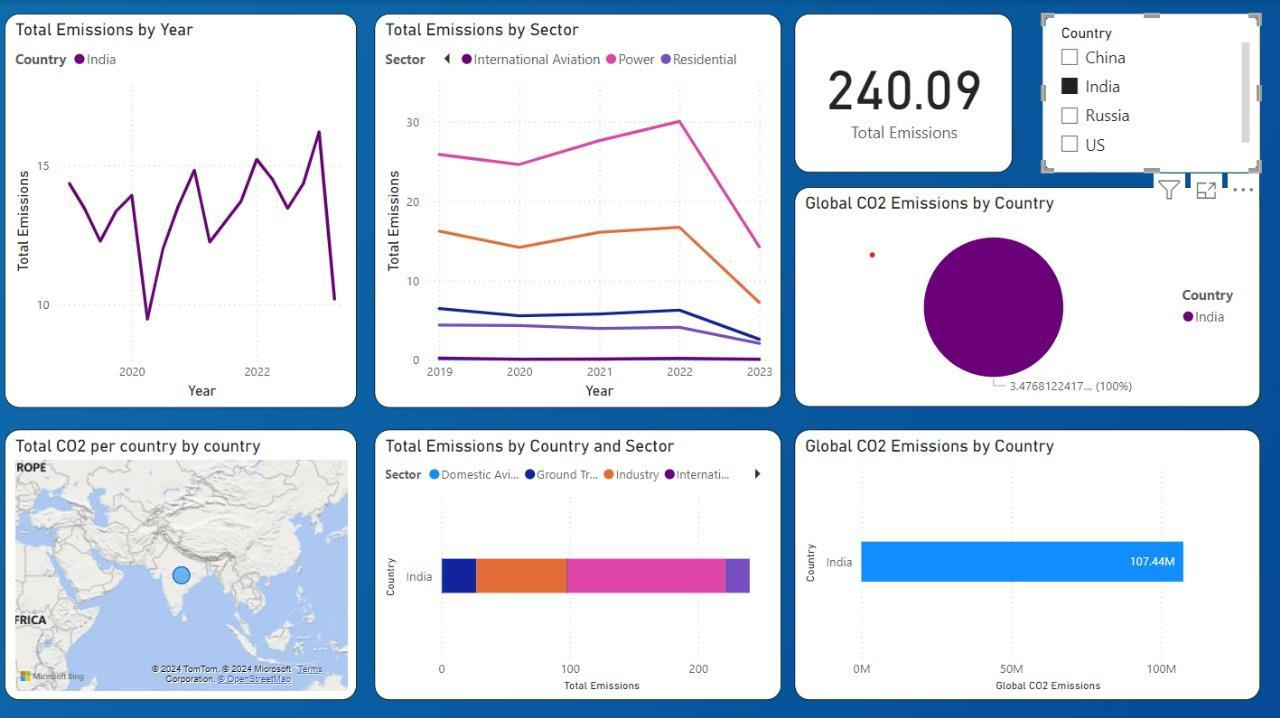
\includegraphics[width=426.8pt,height=239.53pt]{latexImage_8ad5b3d6f5a30354ce1067509860a24c.png}}
\put(93,-677.89){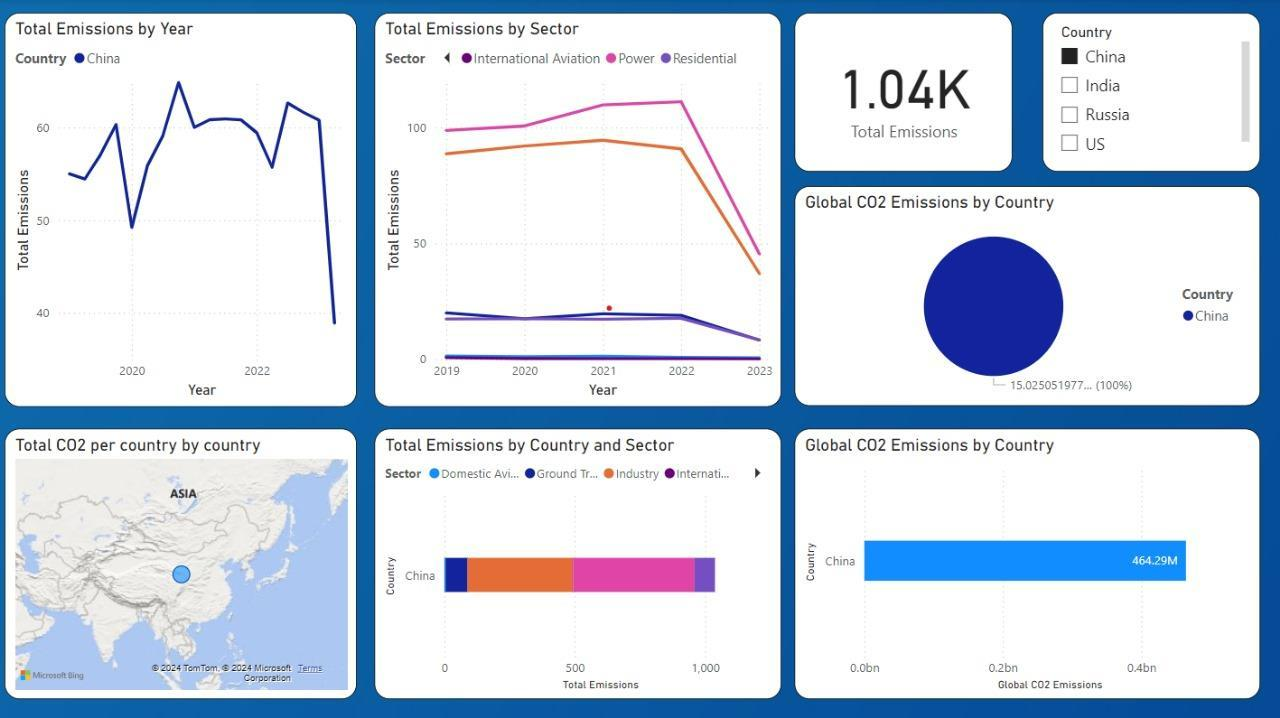
\includegraphics[width=432.08pt,height=242.4pt]{latexImage_97127379ae70040c3f35f5395e73c1e8.png}}
\end{picture}
\newpage
\begin{tikzpicture}[overlay]\path(0pt,0pt);\end{tikzpicture}
\begin{picture}(-5,0)(2.5,0)
\put(21.6,-35.35999){\fontsize{9.96}{1}\usefont{T1}{cmr}{m}{n}\selectfont\color{color_29791}  Breaking the Carbon Curve                                                                                                                                                  AY 2024-25 }
\end{picture}
\begin{tikzpicture}[overlay]
\path(0pt,0pt);
\filldraw[color_156561][even odd rule]
(20.16pt, -42.91998pt) -- (561.8199pt, -42.91998pt)
 -- (561.8199pt, -42.91998pt)
 -- (561.8199pt, -39.91998pt)
 -- (561.8199pt, -39.91998pt)
 -- (20.16pt, -39.91998pt) -- cycle
;
\filldraw[color_156561][even odd rule]
(20.16pt, -39.20001pt) -- (561.8199pt, -39.20001pt)
 -- (561.8199pt, -39.20001pt)
 -- (561.8199pt, -38.48004pt)
 -- (561.8199pt, -38.48004pt)
 -- (20.16pt, -38.48004pt) -- cycle
;
\end{tikzpicture}
\begin{picture}(-5,0)(2.5,0)
\put(291.05,-53.47998){\fontsize{11.04}{1}\usefont{T1}{cmr}{m}{n}\selectfont\color{color_29791} }
\put(21.6,-743.96){\fontsize{9.96}{1}\usefont{T1}{cmr}{m}{n}\selectfont\color{color_29791}     Dept. of CSE, DSCE                                                                                                                                                                          19 }
\end{picture}
\begin{tikzpicture}[overlay]
\path(0pt,0pt);
\filldraw[color_156561][even odd rule]
(20.16pt, -732.176pt) -- (568.92pt, -732.176pt)
 -- (568.92pt, -732.176pt)
 -- (568.92pt, -729.176pt)
 -- (568.92pt, -729.176pt)
 -- (20.16pt, -729.176pt) -- cycle
;
\filldraw[color_156561][even odd rule]
(20.16pt, -733.616pt) -- (568.92pt, -733.616pt)
 -- (568.92pt, -733.616pt)
 -- (568.92pt, -732.896pt)
 -- (568.92pt, -732.896pt)
 -- (20.16pt, -732.896pt) -- cycle
;
\end{tikzpicture}
\begin{picture}(-5,0)(2.5,0)
\put(93.02,-73.17999){\fontsize{12}{1}\usefont{T1}{cmr}{m}{n}\selectfont\color{color_29791} }
\put(75.024,-93.82001){\fontsize{12}{1}\usefont{T1}{cmr}{m}{n}\selectfont\color{color_29791}➢ Sectors Examined: }
\put(75.024,-115.54){\fontsize{12}{1}\usefont{T1}{cmr}{m}{n}\selectfont\color{color_29791}• Power: Major emissions from electricity generation using fossil fuels. }
\put(75.024,-137.14){\fontsize{12}{1}\usefont{T1}{cmr}{m}{n}\selectfont\color{color_29791}• Industry: Energy-intensive processes like manufacturing and construction. }
\put(75.024,-158.62){\fontsize{12}{1}\usefont{T1}{cmr}{m}{n}\selectfont\color{color_29791}• Ground Transport: Emissions from road vehicles. }
\put(75.024,-180.22){\fontsize{12}{1}\usefont{T1}{cmr}{m}{n}\selectfont\color{color_29791}• Domestic Aviation: Relatively small share but high emissions per passenger-mile. }
\put(75.024,-201.82){\fontsize{12}{1}\usefont{T1}{cmr}{m}{n}\selectfont\color{color_29791}• Residential: Energy use in homes, dependent on energy sources like coal or renewables. }
\put(57.024,-230.38){\fontsize{12}{1}\usefont{T1}{cmr}{m}{n}\selectfont\color{color_29791}4.3.4 Insights from Visualizations  }
\put(75.024,-259.09){\fontsize{12}{1}\usefont{T1}{cmr}{m}{n}\selectfont\color{color_29791}➢ Country-Wise Emission Trends }
\put(75.024,-280.81){\fontsize{12}{1}\usefont{T1}{cmr}{m}{n}\selectfont\color{color_29791}• Observation: Significant reductions in emissions in 2023, particularly in China and }
\put(93.02,-301.33){\fontsize{12}{1}\usefont{T1}{cmr}{m}{n}\selectfont\color{color_29791}globally. }
\put(75.024,-323.05){\fontsize{12}{1}\usefont{T1}{cmr}{m}{n}\selectfont\color{color_29791}• Real-World Implications: These reductions likely reflect economic shifts, renewable }
\put(93.02,-343.57){\fontsize{12}{1}\usefont{T1}{cmr}{m}{n}\selectfont\color{color_29791}energy adoption, and policy interventions. }
\put(75.024,-364.33){\fontsize{12}{1}\usefont{T1}{cmr}{m}{n}\selectfont\color{color_29791}➢ Sectoral Emission Trends }
\put(75.024,-385.93){\fontsize{12}{1}\usefont{T1}{cmr}{m}{n}\selectfont\color{color_29791}• Observation: Declines in the Power and Industry sectors, while Ground Transport and }
\put(93.02,-406.59){\fontsize{12}{1}\usefont{T1}{cmr}{m}{n}\selectfont\color{color_29791}Domestic Aviation remained stagnant. }
\put(75.024,-428.31){\fontsize{12}{1}\usefont{T1}{cmr}{m}{n}\selectfont\color{color_29791}• Real-World Implications: Sustained focus on renewable energy and investments in electric }
\put(93.02,-448.83){\fontsize{12}{1}\usefont{T1}{cmr}{m}{n}\selectfont\color{color_29791}mobility are essential. }
\put(57.024,-477.51){\fontsize{12}{1}\usefont{T1}{cmr}{m}{n}\selectfont\color{color_29791} }
\put(75.024,-506.19){\fontsize{12}{1}\usefont{T1}{cmr}{m}{n}\selectfont\color{color_29791}➢ Global Contributions }
\put(75.024,-527.91){\fontsize{12}{1}\usefont{T1}{cmr}{m}{n}\selectfont\color{color_29791}• Observation: The World (63\%) dominates emissions, with China, the US, and India as top }
\put(93.02,-548.55){\fontsize{12}{1}\usefont{T1}{cmr}{m}{n}\selectfont\color{color_29791}individual contributors. }
\put(75.024,-570.15){\fontsize{12}{1}\usefont{T1}{cmr}{m}{n}\selectfont\color{color_29791}• Real-World Implications: International cooperation targeting these nations is critical to }
\put(93.02,-590.82){\fontsize{12}{1}\usefont{T1}{cmr}{m}{n}\selectfont\color{color_29791}meeting global climate goals. }
\put(57.024,-619.5){\fontsize{12}{1}\usefont{T1}{cmr}{m}{n}\selectfont\color{color_29791} }
\put(75.024,-648.18){\fontsize{12}{1}\usefont{T1}{cmr}{m}{n}\selectfont\color{color_29791}➢ Sectoral Contributions by Country }
\put(75.024,-669.9){\fontsize{12}{1}\usefont{T1}{cmr}{m}{n}\selectfont\color{color_29791}• Observation: The Power sector is the largest contributor across all countries, with Domestic }
\put(93.02,-690.416){\fontsize{12}{1}\usefont{T1}{cmr}{m}{n}\selectfont\color{color_29791}Aviation the smallest. }
\end{picture}
\newpage
\begin{tikzpicture}[overlay]\path(0pt,0pt);\end{tikzpicture}
\begin{picture}(-5,0)(2.5,0)
\put(21.6,-35.35999){\fontsize{9.96}{1}\usefont{T1}{cmr}{m}{n}\selectfont\color{color_29791}  Breaking the Carbon Curve                                                                                                                                                  AY 2024-25 }
\end{picture}
\begin{tikzpicture}[overlay]
\path(0pt,0pt);
\filldraw[color_156561][even odd rule]
(20.16pt, -42.91998pt) -- (561.8199pt, -42.91998pt)
 -- (561.8199pt, -42.91998pt)
 -- (561.8199pt, -39.91998pt)
 -- (561.8199pt, -39.91998pt)
 -- (20.16pt, -39.91998pt) -- cycle
;
\filldraw[color_156561][even odd rule]
(20.16pt, -39.20001pt) -- (561.8199pt, -39.20001pt)
 -- (561.8199pt, -39.20001pt)
 -- (561.8199pt, -38.48004pt)
 -- (561.8199pt, -38.48004pt)
 -- (20.16pt, -38.48004pt) -- cycle
;
\end{tikzpicture}
\begin{picture}(-5,0)(2.5,0)
\put(291.05,-53.47998){\fontsize{11.04}{1}\usefont{T1}{cmr}{m}{n}\selectfont\color{color_29791} }
\put(21.6,-743.96){\fontsize{9.96}{1}\usefont{T1}{cmr}{m}{n}\selectfont\color{color_29791}     Dept. of CSE, DSCE                                                                                                                                                                          20 }
\end{picture}
\begin{tikzpicture}[overlay]
\path(0pt,0pt);
\filldraw[color_156561][even odd rule]
(20.16pt, -732.176pt) -- (568.92pt, -732.176pt)
 -- (568.92pt, -732.176pt)
 -- (568.92pt, -729.176pt)
 -- (568.92pt, -729.176pt)
 -- (20.16pt, -729.176pt) -- cycle
;
\filldraw[color_156561][even odd rule]
(20.16pt, -733.616pt) -- (568.92pt, -733.616pt)
 -- (568.92pt, -733.616pt)
 -- (568.92pt, -732.896pt)
 -- (568.92pt, -732.896pt)
 -- (20.16pt, -732.896pt) -- cycle
;
\end{tikzpicture}
\begin{picture}(-5,0)(2.5,0)
\put(93.02,-73.17999){\fontsize{12}{1}\usefont{T1}{cmr}{m}{n}\selectfont\color{color_29791} }
\put(75.024,-94.78003){\fontsize{12}{1}\usefont{T1}{cmr}{m}{n}\selectfont\color{color_29791}• Real-World Implications: Countries should prioritize decarbonizing power generation and }
\put(93.02,-115.42){\fontsize{12}{1}\usefont{T1}{cmr}{m}{n}\selectfont\color{color_29791}improving energy efficiency in industries. }
\put(93.02,-136.18){\fontsize{12}{1}\usefont{T1}{cmr}{m}{n}\selectfont\color{color_29791} }
\put(93.02,-151.06){\fontsize{12}{1}\usefont{T1}{cmr}{m}{n}\selectfont\color{color_29791} }
\put(93.02,-171.7){\fontsize{12}{1}\usefont{T1}{cmr}{m}{n}\selectfont\color{color_29791} }
\put(516.94,-415.35){\fontsize{12}{1}\usefont{T1}{cmr}{m}{n}\selectfont\color{color_29791} }
\put(196.49,-433.23){\fontsize{12}{1}\usefont{T1}{cmr}{m}{n}\selectfont\color{color_29791}Figure 4.3.3: Insights of US on CO2 emissions }
\put(309.07,-453.87){\fontsize{12}{1}\usefont{T1}{cmr}{m}{n}\selectfont\color{color_29791} }
\put(57.024,-482.55){\fontsize{12}{1}\usefont{T1}{cmr}{m}{n}\selectfont\color{color_29791}4.3.5 Future Policies for India }
\put(75.024,-512.19){\fontsize{12}{1}\usefont{T1}{cmr}{m}{n}\selectfont\color{color_29791}• Power Sector: Expand renewable energy infrastructure and encourage decentralized }
\put(93.02,-532.83){\fontsize{12}{1}\usefont{T1}{cmr}{m}{n}\selectfont\color{color_29791}systems like rooftop solar. }
\put(75.024,-554.55){\fontsize{12}{1}\usefont{T1}{cmr}{m}{n}\selectfont\color{color_29791}• Industry: Promote energy-efficient technologies and green certifications. }
\put(75.024,-576.06){\fontsize{12}{1}\usefont{T1}{cmr}{m}{n}\selectfont\color{color_29791}• Transport: Invest in public transport, electric vehicles, and biofuels. }
\put(75.024,-597.66){\fontsize{12}{1}\usefont{T1}{cmr}{m}{n}\selectfont\color{color_29791}• Residential: Mandate energy-efficient building codes and incentivize green housing }
\put(93.02,-618.3){\fontsize{12}{1}\usefont{T1}{cmr}{m}{n}\selectfont\color{color_29791}projects. }
\put(57.024,-646.98){\fontsize{12}{1}\usefont{T1}{cmr}{m}{n}\selectfont\color{color_29791}By focusing on these areas, India can balance economic growth with sustainability, reducing its }
\put(57.024,-667.62){\fontsize{12}{1}\usefont{T1}{cmr}{m}{n}\selectfont\color{color_29791}emissions and contributing to a healthier environment. }
\put(57.024,-696.296){\fontsize{12}{1}\usefont{T1}{cmr}{m}{n}\selectfont\color{color_29791} }
\put(101.07,-415.09){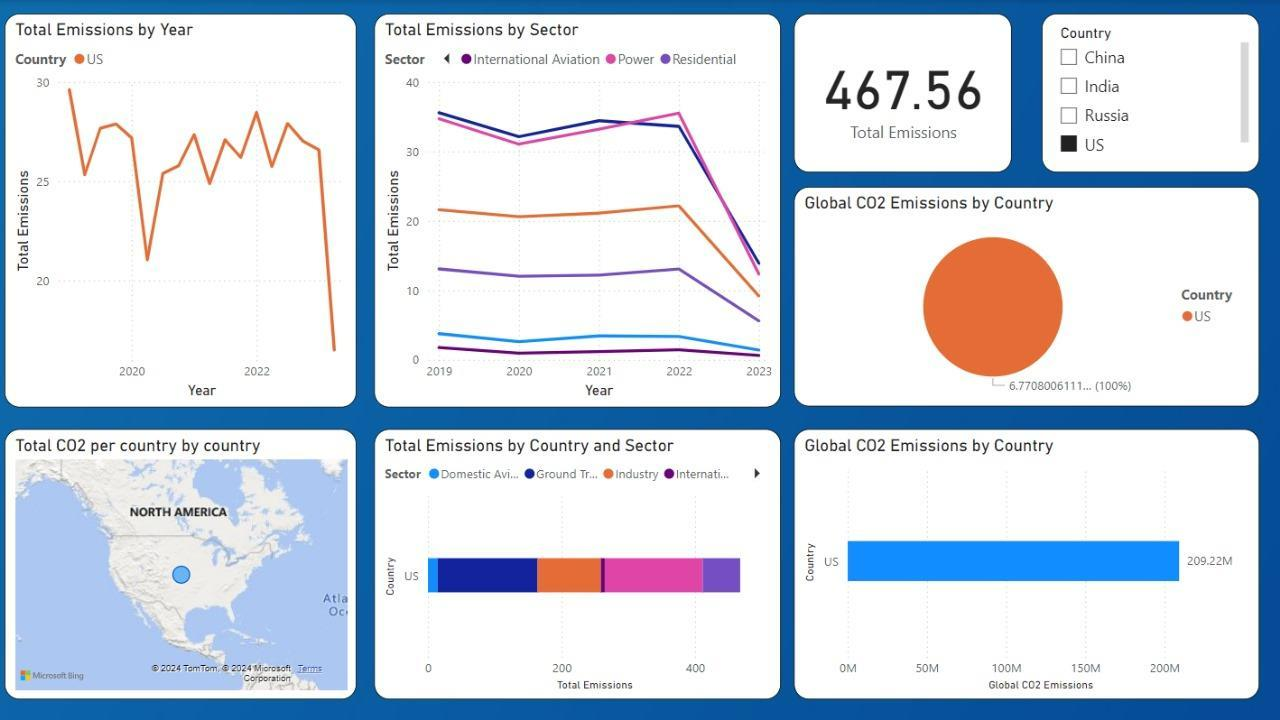
\includegraphics[width=415.81pt,height=233.85pt]{latexImage_86605d6faacfa2b488ab1aff7951d282.png}}
\end{picture}
\newpage
\begin{tikzpicture}[overlay]\path(0pt,0pt);\end{tikzpicture}
\begin{picture}(-5,0)(2.5,0)
\put(21.6,-35.35999){\fontsize{9.96}{1}\usefont{T1}{cmr}{m}{n}\selectfont\color{color_29791}  Breaking the Carbon Curve                                                                                                                                                  AY 2024-25 }
\end{picture}
\begin{tikzpicture}[overlay]
\path(0pt,0pt);
\filldraw[color_156561][even odd rule]
(20.16pt, -42.91998pt) -- (561.8199pt, -42.91998pt)
 -- (561.8199pt, -42.91998pt)
 -- (561.8199pt, -39.91998pt)
 -- (561.8199pt, -39.91998pt)
 -- (20.16pt, -39.91998pt) -- cycle
;
\filldraw[color_156561][even odd rule]
(20.16pt, -39.20001pt) -- (561.8199pt, -39.20001pt)
 -- (561.8199pt, -39.20001pt)
 -- (561.8199pt, -38.48004pt)
 -- (561.8199pt, -38.48004pt)
 -- (20.16pt, -38.48004pt) -- cycle
;
\end{tikzpicture}
\begin{picture}(-5,0)(2.5,0)
\put(291.05,-53.47998){\fontsize{11.04}{1}\usefont{T1}{cmr}{m}{n}\selectfont\color{color_29791} }
\put(21.6,-743.96){\fontsize{9.96}{1}\usefont{T1}{cmr}{m}{n}\selectfont\color{color_29791}     Dept. of CSE, DSCE                                                                                                                                                                          21 }
\end{picture}
\begin{tikzpicture}[overlay]
\path(0pt,0pt);
\filldraw[color_156561][even odd rule]
(20.16pt, -732.176pt) -- (568.92pt, -732.176pt)
 -- (568.92pt, -732.176pt)
 -- (568.92pt, -729.176pt)
 -- (568.92pt, -729.176pt)
 -- (20.16pt, -729.176pt) -- cycle
;
\filldraw[color_156561][even odd rule]
(20.16pt, -733.616pt) -- (568.92pt, -733.616pt)
 -- (568.92pt, -733.616pt)
 -- (568.92pt, -732.896pt)
 -- (568.92pt, -732.896pt)
 -- (20.16pt, -732.896pt) -- cycle
;
\end{tikzpicture}
\begin{picture}(-5,0)(2.5,0)
\put(57.024,-73.17999){\fontsize{12}{1}\usefont{T1}{cmr}{m}{n}\selectfont\color{color_29791}4.3.6 Integration of Data Analysis and Visualizations with the Project }
\put(57.024,-96.09998){\fontsize{12}{1}\usefont{T1}{cmr}{m}{n}\selectfont\color{color_29791} }
\put(57.024,-119.02){\fontsize{12}{1}\usefont{T1}{cmr}{m}{n}\selectfont\color{color_29791}Data analysis and visualizations form a vital foundation of the CO2 emissions project, connecting }
\put(57.024,-139.66){\fontsize{12}{1}\usefont{T1}{cmr}{m}{n}\selectfont\color{color_29791}raw data to actionable insights. This section highlights how these elements contribute to achieving }
\put(57.024,-160.3){\fontsize{12}{1}\usefont{T1}{cmr}{m}{n}\selectfont\color{color_29791}the project’s objectives and ensuring its real-world relevance. }
\put(57.024,-189.1){\fontsize{12}{1}\usefont{T1}{cmr}{m}{n}\selectfont\color{color_29791}1. Contextualizing the Problem }
\put(57.024,-217.78){\fontsize{12}{1}\usefont{T1}{cmr}{m}{n}\selectfont\color{color_29791}This project focuses on analysing and forecasting CO2 emissions to support sustainable practices }
\put(57.024,-238.45){\fontsize{12}{1}\usefont{T1}{cmr}{m}{n}\selectfont\color{color_29791}and policies. Visualizations play a key role by: }
\put(75.024,-268.09){\fontsize{12}{1}\usefont{T1}{cmr}{m}{n}\selectfont\color{color_29791}• Quantifying Emission Patterns: Providing a clear picture of trends across countries and }
\put(93.02,-288.73){\fontsize{12}{1}\usefont{T1}{cmr}{m}{n}\selectfont\color{color_29791}sectors, essential for identifying priority areas. }
\put(75.024,-310.45){\fontsize{12}{1}\usefont{T1}{cmr}{m}{n}\selectfont\color{color_29791}• Highlighting Key Contributors: Pinpointing major emitters helps direct efforts where }
\put(93.02,-330.97){\fontsize{12}{1}\usefont{T1}{cmr}{m}{n}\selectfont\color{color_29791}they will have the most impact. }
\put(75.024,-352.69){\fontsize{12}{1}\usefont{T1}{cmr}{m}{n}\selectfont\color{color_29791}• Tracking Long-Term Trends: Time-series analyses reveal shifts in emissions, forming a }
\put(93.02,-373.21){\fontsize{12}{1}\usefont{T1}{cmr}{m}{n}\selectfont\color{color_29791}basis for predictive models. }
\put(57.024,-402.01){\fontsize{12}{1}\usefont{T1}{cmr}{m}{n}\selectfont\color{color_29791}2. Enhancing Forecasting Accuracy }
\put(57.024,-430.71){\fontsize{12}{1}\usefont{T1}{cmr}{m}{n}\selectfont\color{color_29791}Data visualizations support the development of time-series forecasting models by: }
\put(75.024,-460.35){\fontsize{12}{1}\usefont{T1}{cmr}{m}{n}\selectfont\color{color_29791}• Identifying Trends: Insights, such as sudden emission declines, inform model }
\put(93.02,-480.99){\fontsize{12}{1}\usefont{T1}{cmr}{m}{n}\selectfont\color{color_29791}assumptions and improve precision. }
\put(75.024,-502.59){\fontsize{12}{1}\usefont{T1}{cmr}{m}{n}\selectfont\color{color_29791}• Sectoral Analysis: Breaking down emissions by sector helps models incorporate specific }
\put(93.02,-523.23){\fontsize{12}{1}\usefont{T1}{cmr}{m}{n}\selectfont\color{color_29791}dynamics, making predictions more actionable. }
\put(75.024,-544.83){\fontsize{12}{1}\usefont{T1}{cmr}{m}{n}\selectfont\color{color_29791}• Focusing Data: Prioritizing data from key contributors like China and India ensures }
\put(93.02,-565.47){\fontsize{12}{1}\usefont{T1}{cmr}{m}{n}\selectfont\color{color_29791}meaningful insights while optimizing resources. }
\put(57.024,-594.18){\fontsize{12}{1}\usefont{T1}{cmr}{m}{n}\selectfont\color{color_29791}3. Supporting Policy and Decision-Making }
\put(57.024,-622.86){\fontsize{12}{1}\usefont{T1}{cmr}{m}{n}\selectfont\color{color_29791}The visualizations empower decision-makers to: }
\put(75.024,-652.5){\fontsize{12}{1}\usefont{T1}{cmr}{m}{n}\selectfont\color{color_29791}• Design Sector-Specific Policies: For example, stagnant emissions in ground transportation }
\put(93.02,-673.14){\fontsize{12}{1}\usefont{T1}{cmr}{m}{n}\selectfont\color{color_29791}highlight the need for electric vehicle adoption and better public transit. }
\end{picture}
\newpage
\begin{tikzpicture}[overlay]\path(0pt,0pt);\end{tikzpicture}
\begin{picture}(-5,0)(2.5,0)
\put(21.6,-35.35999){\fontsize{9.96}{1}\usefont{T1}{cmr}{m}{n}\selectfont\color{color_29791}  Breaking the Carbon Curve                                                                                                                                                  AY 2024-25 }
\end{picture}
\begin{tikzpicture}[overlay]
\path(0pt,0pt);
\filldraw[color_156561][even odd rule]
(20.16pt, -42.91998pt) -- (561.8199pt, -42.91998pt)
 -- (561.8199pt, -42.91998pt)
 -- (561.8199pt, -39.91998pt)
 -- (561.8199pt, -39.91998pt)
 -- (20.16pt, -39.91998pt) -- cycle
;
\filldraw[color_156561][even odd rule]
(20.16pt, -39.20001pt) -- (561.8199pt, -39.20001pt)
 -- (561.8199pt, -39.20001pt)
 -- (561.8199pt, -38.48004pt)
 -- (561.8199pt, -38.48004pt)
 -- (20.16pt, -38.48004pt) -- cycle
;
\end{tikzpicture}
\begin{picture}(-5,0)(2.5,0)
\put(291.05,-53.47998){\fontsize{11.04}{1}\usefont{T1}{cmr}{m}{n}\selectfont\color{color_29791} }
\put(21.6,-743.96){\fontsize{9.96}{1}\usefont{T1}{cmr}{m}{n}\selectfont\color{color_29791}     Dept. of CSE, DSCE                                                                                                                                                                          22 }
\end{picture}
\begin{tikzpicture}[overlay]
\path(0pt,0pt);
\filldraw[color_156561][even odd rule]
(20.16pt, -732.176pt) -- (568.92pt, -732.176pt)
 -- (568.92pt, -732.176pt)
 -- (568.92pt, -729.176pt)
 -- (568.92pt, -729.176pt)
 -- (20.16pt, -729.176pt) -- cycle
;
\filldraw[color_156561][even odd rule]
(20.16pt, -733.616pt) -- (568.92pt, -733.616pt)
 -- (568.92pt, -733.616pt)
 -- (568.92pt, -732.896pt)
 -- (568.92pt, -732.896pt)
 -- (20.16pt, -732.896pt) -- cycle
;
\end{tikzpicture}
\begin{picture}(-5,0)(2.5,0)
\put(75.024,-74.14001){\fontsize{12}{1}\usefont{T1}{cmr}{m}{n}\selectfont\color{color_29791}• Benchmark Progress: Countries can compare trends with peers to identify effective }
\put(93.02,-94.78003){\fontsize{12}{1}\usefont{T1}{cmr}{m}{n}\selectfont\color{color_29791}strategies. }
\put(75.024,-116.38){\fontsize{12}{1}\usefont{T1}{cmr}{m}{n}\selectfont\color{color_29791}• Set Achievable Goals: Visualized global contributions help nations align with initiatives }
\put(93.02,-137.02){\fontsize{12}{1}\usefont{T1}{cmr}{m}{n}\selectfont\color{color_29791}like the Paris Agreement. }
\put(57.024,-165.7){\fontsize{12}{1}\usefont{T1}{cmr}{m}{n}\selectfont\color{color_29791}4. Enhancing Explainability in AI Models }
\put(57.024,-194.38){\fontsize{12}{1}\usefont{T1}{cmr}{m}{n}\selectfont\color{color_29791}Visualizations complement explainable AI methods by: }
\put(75.024,-224.02){\fontsize{12}{1}\usefont{T1}{cmr}{m}{n}\selectfont\color{color_29791}• Establishing Baselines: Historical trends provide a reference for validating model outputs. }
\put(75.024,-245.65){\fontsize{12}{1}\usefont{T1}{cmr}{m}{n}\selectfont\color{color_29791}• Simplifying Insights: Dashboards make complex AI-generated results accessible to non-}
\put(93.02,-266.29){\fontsize{12}{1}\usefont{T1}{cmr}{m}{n}\selectfont\color{color_29791}technical stakeholders. }
\put(75.024,-287.89){\fontsize{12}{1}\usefont{T1}{cmr}{m}{n}\selectfont\color{color_29791}• Identifying Key Features: Sectoral and country-level data guide model feature selection, }
\put(93.02,-308.53){\fontsize{12}{1}\usefont{T1}{cmr}{m}{n}\selectfont\color{color_29791}improving transparency. }
\put(57.024,-337.21){\fontsize{12}{1}\usefont{T1}{cmr}{m}{n}\selectfont\color{color_29791}5. Real-World Applications }
\put(75.024,-366.85){\fontsize{12}{1}\usefont{T1}{cmr}{m}{n}\selectfont\color{color_29791}• For Policymakers: Develop targeted climate policies and monitor their effectiveness }
\put(93.02,-387.49){\fontsize{12}{1}\usefont{T1}{cmr}{m}{n}\selectfont\color{color_29791}through real-time dashboards. }
\put(75.024,-409.11){\fontsize{12}{1}\usefont{T1}{cmr}{m}{n}\selectfont\color{color_29791}• For Businesses: Align operations with sustainability goals and identify opportunities in }
\put(93.02,-429.75){\fontsize{12}{1}\usefont{T1}{cmr}{m}{n}\selectfont\color{color_29791}renewable energy and eco-friendly technologies. }
\put(75.024,-451.35){\fontsize{12}{1}\usefont{T1}{cmr}{m}{n}\selectfont\color{color_29791}• For Researchers and Educators: Use visual insights for academic studies, public }
\put(93.02,-471.99){\fontsize{12}{1}\usefont{T1}{cmr}{m}{n}\selectfont\color{color_29791}awareness campaigns, and promoting the importance of emissions reduction }
\put(57.024,-500.67){\fontsize{12}{1}\usefont{T1}{cmr}{m}{n}\selectfont\color{color_29791}Data analysis and visualizations are the backbone of this project, ensuring clarity and driving }
\put(57.024,-521.43){\fontsize{12}{1}\usefont{T1}{cmr}{m}{n}\selectfont\color{color_29791}informed decisions. They connect forecasting and modelling efforts to practical applications, }
\put(57.024,-542.07){\fontsize{12}{1}\usefont{T1}{cmr}{m}{n}\selectfont\color{color_29791}enabling meaningful contributions to global sustainability goals. These insights are not just }
\put(57.024,-562.83){\fontsize{12}{1}\usefont{T1}{cmr}{m}{n}\selectfont\color{color_29791}informative but transformative, supporting collaborative action to tackle CO2 emissions }
\put(57.024,-583.5){\fontsize{12}{1}\usefont{T1}{cmr}{m}{n}\selectfont\color{color_29791}effectively. }
\put(57.024,-612.18){\fontsize{12}{1}\usefont{T1}{cmr}{m}{n}\selectfont\color{color_29791} }
\put(57.024,-640.86){\fontsize{12}{1}\usefont{T1}{cmr}{m}{n}\selectfont\color{color_29791} }
\put(57.024,-669.66){\fontsize{12}{1}\usefont{T1}{cmr}{m}{n}\selectfont\color{color_29791} }
\put(57.024,-698.336){\fontsize{12}{1}\usefont{T1}{cmr}{m}{n}\selectfont\color{color_29791} }
\end{picture}
\newpage
\begin{tikzpicture}[overlay]\path(0pt,0pt);\end{tikzpicture}
\begin{picture}(-5,0)(2.5,0)
\put(21.6,-35.35999){\fontsize{9.96}{1}\usefont{T1}{cmr}{m}{n}\selectfont\color{color_29791}  Breaking the Carbon Curve                                                                                                                                                  AY 2024-25 }
\end{picture}
\begin{tikzpicture}[overlay]
\path(0pt,0pt);
\filldraw[color_156561][even odd rule]
(20.16pt, -42.91998pt) -- (561.8199pt, -42.91998pt)
 -- (561.8199pt, -42.91998pt)
 -- (561.8199pt, -39.91998pt)
 -- (561.8199pt, -39.91998pt)
 -- (20.16pt, -39.91998pt) -- cycle
;
\filldraw[color_156561][even odd rule]
(20.16pt, -39.20001pt) -- (561.8199pt, -39.20001pt)
 -- (561.8199pt, -39.20001pt)
 -- (561.8199pt, -38.48004pt)
 -- (561.8199pt, -38.48004pt)
 -- (20.16pt, -38.48004pt) -- cycle
;
\end{tikzpicture}
\begin{picture}(-5,0)(2.5,0)
\put(291.05,-53.47998){\fontsize{11.04}{1}\usefont{T1}{cmr}{m}{n}\selectfont\color{color_29791} }
\put(21.6,-743.96){\fontsize{9.96}{1}\usefont{T1}{cmr}{m}{n}\selectfont\color{color_29791}     Dept. of CSE, DSCE                                                                                                                                                                          23 }
\end{picture}
\begin{tikzpicture}[overlay]
\path(0pt,0pt);
\filldraw[color_156561][even odd rule]
(20.16pt, -732.176pt) -- (568.92pt, -732.176pt)
 -- (568.92pt, -732.176pt)
 -- (568.92pt, -729.176pt)
 -- (568.92pt, -729.176pt)
 -- (20.16pt, -729.176pt) -- cycle
;
\filldraw[color_156561][even odd rule]
(20.16pt, -733.616pt) -- (568.92pt, -733.616pt)
 -- (568.92pt, -733.616pt)
 -- (568.92pt, -732.896pt)
 -- (568.92pt, -732.896pt)
 -- (20.16pt, -732.896pt) -- cycle
;
\end{tikzpicture}
\begin{picture}(-5,0)(2.5,0)
\put(57.024,-73.17999){\fontsize{12}{1}\usefont{T1}{cmr}{m}{n}\selectfont\color{color_29791} }
\put(57.024,-105.7){\fontsize{15.96}{1}\usefont{T1}{cmr}{m}{n}\selectfont\color{color_29791}4.4 Ecolens }
\put(57.024,-137.5){\fontsize{12}{1}\usefont{T1}{cmr}{m}{n}\selectfont\color{color_29791}4.4.1 Integration of the LLM-Powered CO2 Emissions Assistant with the Project }
\put(57.024,-166.18){\fontsize{12}{1}\usefont{T1}{cmr}{m}{n}\selectfont\color{color_29791}The Personal CO2 Emissions Assistant, designed using the Retrieval Augmented Generation }
\put(57.024,-186.82){\fontsize{12}{1}\usefont{T1}{cmr}{m}{n}\selectfont\color{color_29791}(RAG) methodology, is an integral part of this project. It offers personalized, actionable }
\put(57.024,-207.58){\fontsize{12}{1}\usefont{T1}{cmr}{m}{n}\selectfont\color{color_29791}recommendations to help individuals reduce their carbon footprint. This section explains the key }
\put(57.024,-228.22){\fontsize{12}{1}\usefont{T1}{cmr}{m}{n}\selectfont\color{color_29791}components, functionality, and value this assistant adds to the project. }
\put(525.1,-489.27){\fontsize{12}{1}\usefont{T1}{cmr}{m}{n}\selectfont\color{color_29791} }
\put(225.41,-515.07){\fontsize{12}{1}\usefont{T1}{cmr}{m}{n}\selectfont\color{color_29791}Figure 4.4.1: UI of Ecolens }
\put(57.024,-543.75){\fontsize{12}{1}\usefont{T1}{cmr}{m}{n}\selectfont\color{color_29791}In figure 4.4.1, the user is asked to enter the context and question, the Rag model used here will }
\put(57.024,-564.39){\fontsize{12}{1}\usefont{T1}{cmr}{m}{n}\selectfont\color{color_29791}provide actionable recommendations and ways to reduce emissions rate.  }
\put(57.024,-593.1){\fontsize{12}{1}\usefont{T1}{cmr}{m}{n}\selectfont\color{color_29791}Context: I drive my car to work every day, about 10 kilometres each way.  }
\put(57.024,-621.9){\fontsize{12}{1}\usefont{T1}{cmr}{m}{n}\selectfont\color{color_29791}Question: What are some easy ways I can reduce my carbon footprint based on these habits? }
\put(57.024,-650.58){\fontsize{12}{1}\usefont{T1}{cmr}{m}{n}\selectfont\color{color_29791} }
\put(57.024,-679.26){\fontsize{12}{1}\usefont{T1}{cmr}{m}{n}\selectfont\color{color_29791} }
\put(57,-489.09){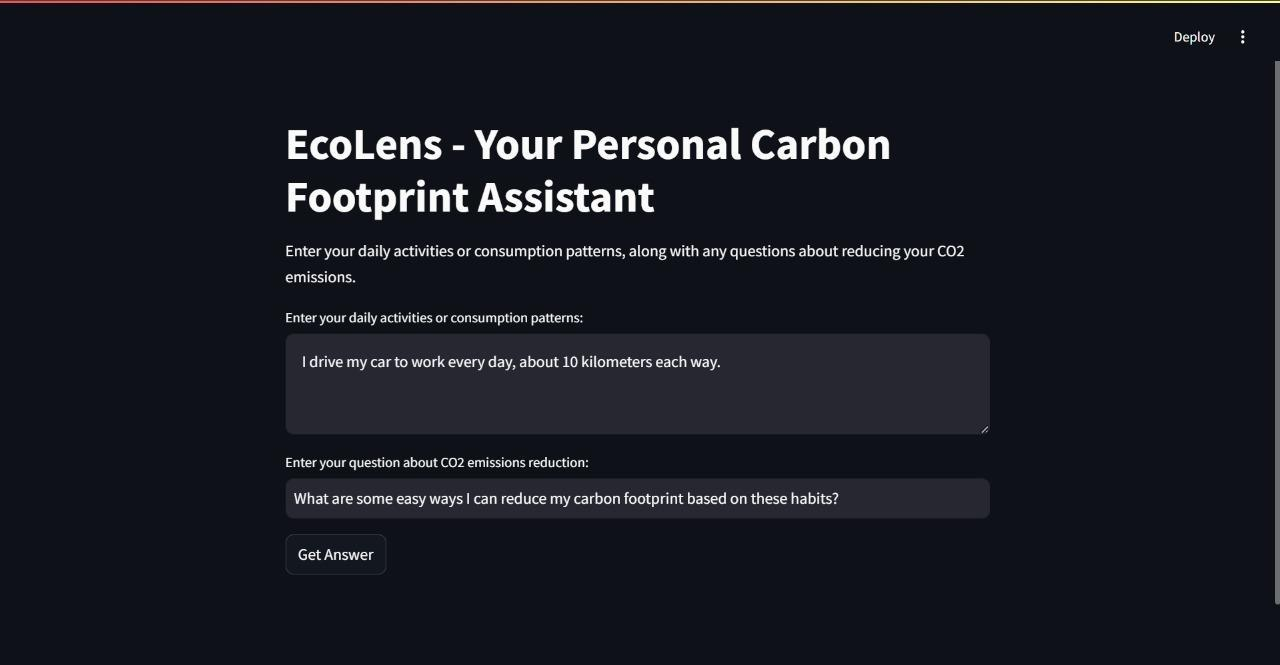
\includegraphics[width=468pt,height=243.3pt]{latexImage_c1df92a0aa33b1d347270fa6d252657d.png}}
\end{picture}
\newpage
\begin{tikzpicture}[overlay]\path(0pt,0pt);\end{tikzpicture}
\begin{picture}(-5,0)(2.5,0)
\put(21.6,-35.35999){\fontsize{9.96}{1}\usefont{T1}{cmr}{m}{n}\selectfont\color{color_29791}  Breaking the Carbon Curve                                                                                                                                                  AY 2024-25 }
\end{picture}
\begin{tikzpicture}[overlay]
\path(0pt,0pt);
\filldraw[color_156561][even odd rule]
(20.16pt, -42.91998pt) -- (561.8199pt, -42.91998pt)
 -- (561.8199pt, -42.91998pt)
 -- (561.8199pt, -39.91998pt)
 -- (561.8199pt, -39.91998pt)
 -- (20.16pt, -39.91998pt) -- cycle
;
\filldraw[color_156561][even odd rule]
(20.16pt, -39.20001pt) -- (561.8199pt, -39.20001pt)
 -- (561.8199pt, -39.20001pt)
 -- (561.8199pt, -38.48004pt)
 -- (561.8199pt, -38.48004pt)
 -- (20.16pt, -38.48004pt) -- cycle
;
\end{tikzpicture}
\begin{picture}(-5,0)(2.5,0)
\put(291.05,-53.47998){\fontsize{11.04}{1}\usefont{T1}{cmr}{m}{n}\selectfont\color{color_29791} }
\put(21.6,-743.96){\fontsize{9.96}{1}\usefont{T1}{cmr}{m}{n}\selectfont\color{color_29791}     Dept. of CSE, DSCE                                                                                                                                                                          24 }
\end{picture}
\begin{tikzpicture}[overlay]
\path(0pt,0pt);
\filldraw[color_156561][even odd rule]
(20.16pt, -732.176pt) -- (568.92pt, -732.176pt)
 -- (568.92pt, -732.176pt)
 -- (568.92pt, -729.176pt)
 -- (568.92pt, -729.176pt)
 -- (20.16pt, -729.176pt) -- cycle
;
\filldraw[color_156561][even odd rule]
(20.16pt, -733.616pt) -- (568.92pt, -733.616pt)
 -- (568.92pt, -733.616pt)
 -- (568.92pt, -732.896pt)
 -- (568.92pt, -732.896pt)
 -- (20.16pt, -732.896pt) -- cycle
;
\end{tikzpicture}
\begin{picture}(-5,0)(2.5,0)
\put(57.024,-73.17999){\fontsize{12}{1}\usefont{T1}{cmr}{m}{n}\selectfont\color{color_29791} }
\put(525.1,-333.73){\fontsize{12}{1}\usefont{T1}{cmr}{m}{n}\selectfont\color{color_29791} }
\put(135.98,-359.65){\fontsize{12}{1}\usefont{T1}{cmr}{m}{n}\selectfont\color{color_29791}Figure 4.4.2: Actionable recommendations and valuable insights }
\put(57.024,-388.33){\fontsize{12}{1}\usefont{T1}{cmr}{m}{n}\selectfont\color{color_29791}Components and Their Roles: }
\put(57.024,-417.03){\fontsize{12}{1}\usefont{T1}{cmr}{m}{n}\selectfont\color{color_29791}1. Groq Llama 3 8B model   }
\put(84.504,-446.67){\fontsize{12}{1}\usefont{T1}{cmr}{m}{n}\selectfont\color{color_29791}• An advanced open-source language model optimized for understanding context and }
\put(102.5,-467.31){\fontsize{12}{1}\usefont{T1}{cmr}{m}{n}\selectfont\color{color_29791}generating high-quality responses tailored to user inputs.   }
\put(57.024,-495.99){\fontsize{12}{1}\usefont{T1}{cmr}{m}{n}\selectfont\color{color_29791}2. FAISS Vector Store   }
\put(84.504,-525.63){\fontsize{12}{1}\usefont{T1}{cmr}{m}{n}\selectfont\color{color_29791}• A high-performance similarity search tool that efficiently retrieves relevant data based on }
\put(102.5,-546.27){\fontsize{12}{1}\usefont{T1}{cmr}{m}{n}\selectfont\color{color_29791}user queries.   }
\put(57.024,-574.98){\fontsize{12}{1}\usefont{T1}{cmr}{m}{n}\selectfont\color{color_29791}3. Hugging Face Embeddings   }
\put(84.504,-604.62){\fontsize{12}{1}\usefont{T1}{cmr}{m}{n}\selectfont\color{color_29791}• A tool for converting textual data into numerical formats, enabling effective matching of }
\put(102.5,-625.26){\fontsize{12}{1}\usefont{T1}{cmr}{m}{n}\selectfont\color{color_29791}user inputs with stored data.   }
\put(57.024,-653.94){\fontsize{12}{1}\usefont{T1}{cmr}{m}{n}\selectfont\color{color_29791}4. LangChain Framework   }
\put(84.504,-683.576){\fontsize{12}{1}\usefont{T1}{cmr}{m}{n}\selectfont\color{color_29791}• A modular framework that integrates different components, ensuring seamless interaction }
\put(102.5,-704.216){\fontsize{12}{1}\usefont{T1}{cmr}{m}{n}\selectfont\color{color_29791}be}
\put(57,-333.2){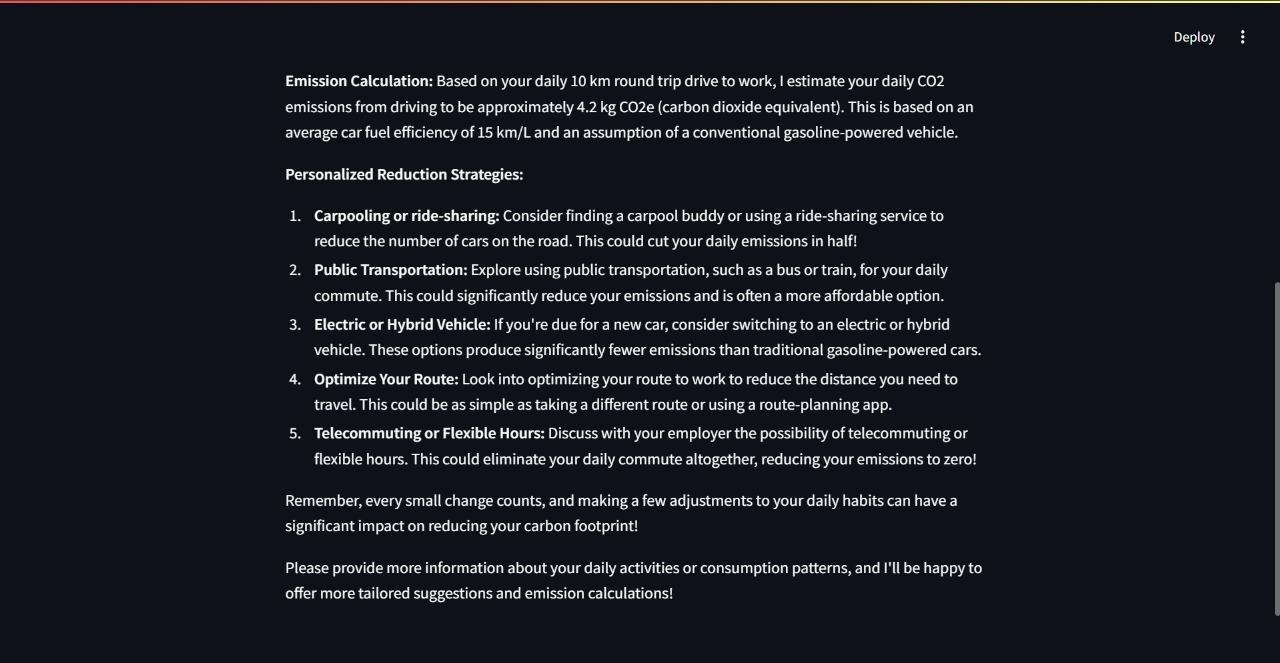
\includegraphics[width=468pt,height=242.5pt]{latexImage_cf59a8291cc996b74bb3505976436e8a.png}}
\end{picture}
\newpage
\begin{tikzpicture}[overlay]\path(0pt,0pt);\end{tikzpicture}
\begin{picture}(-5,0)(2.5,0)
\put(21.6,-35.35999){\fontsize{9.96}{1}\usefont{T1}{cmr}{m}{n}\selectfont\color{color_29791}  Breaking the Carbon Curve                                                                                                                                                  AY 2024-25 }
\end{picture}
\begin{tikzpicture}[overlay]
\path(0pt,0pt);
\filldraw[color_156561][even odd rule]
(20.16pt, -42.91998pt) -- (561.8199pt, -42.91998pt)
 -- (561.8199pt, -42.91998pt)
 -- (561.8199pt, -39.91998pt)
 -- (561.8199pt, -39.91998pt)
 -- (20.16pt, -39.91998pt) -- cycle
;
\filldraw[color_156561][even odd rule]
(20.16pt, -39.20001pt) -- (561.8199pt, -39.20001pt)
 -- (561.8199pt, -39.20001pt)
 -- (561.8199pt, -38.48004pt)
 -- (561.8199pt, -38.48004pt)
 -- (20.16pt, -38.48004pt) -- cycle
;
\end{tikzpicture}
\begin{picture}(-5,0)(2.5,0)
\put(291.05,-53.47998){\fontsize{11.04}{1}\usefont{T1}{cmr}{m}{n}\selectfont\color{color_29791} }
\put(21.6,-743.96){\fontsize{9.96}{1}\usefont{T1}{cmr}{m}{n}\selectfont\color{color_29791}     Dept. of CSE, DSCE                                                                                                                                                                          25 }
\end{picture}
\begin{tikzpicture}[overlay]
\path(0pt,0pt);
\filldraw[color_156561][even odd rule]
(20.16pt, -732.176pt) -- (568.92pt, -732.176pt)
 -- (568.92pt, -732.176pt)
 -- (568.92pt, -729.176pt)
 -- (568.92pt, -729.176pt)
 -- (20.16pt, -729.176pt) -- cycle
;
\filldraw[color_156561][even odd rule]
(20.16pt, -733.616pt) -- (568.92pt, -733.616pt)
 -- (568.92pt, -733.616pt)
 -- (568.92pt, -732.896pt)
 -- (568.92pt, -732.896pt)
 -- (20.16pt, -732.896pt) -- cycle
;
\end{tikzpicture}
\begin{picture}(-5,0)(2.5,0)
\put(57.024,-73.17999){\fontsize{12}{1}\usefont{T1}{cmr}{m}{n}\selectfont\color{color_29791}5. Streamlit   }
\put(84.504,-102.82){\fontsize{12}{1}\usefont{T1}{cmr}{m}{n}\selectfont\color{color_29791}• A user-friendly platform for creating interactive web applications, enabling users to input }
\put(102.5,-123.46){\fontsize{12}{1}\usefont{T1}{cmr}{m}{n}\selectfont\color{color_29791}data and view results easily.   }
\put(57.024,-152.14){\fontsize{12}{1}\usefont{T1}{cmr}{m}{n}\selectfont\color{color_29791}6. Prompt Template   }
\put(84.504,-181.78){\fontsize{12}{1}\usefont{T1}{cmr}{m}{n}\selectfont\color{color_29791}• A structured format for queries that ensures the language model generates accurate and }
\put(102.5,-202.42){\fontsize{12}{1}\usefont{T1}{cmr}{m}{n}\selectfont\color{color_29791}focused responses related to CO2 emissions and reduction strategies. }
\put(490.06,-495.99){\fontsize{12}{1}\usefont{T1}{cmr}{m}{n}\selectfont\color{color_29791} }
\put(206.45,-513.87){\fontsize{12}{1}\usefont{T1}{cmr}{m}{n}\selectfont\color{color_29791}Figure 4.4.3: High level overview of ecolens }
\put(57.024,-542.55){\fontsize{12}{1}\usefont{T1}{cmr}{m}{n}\selectfont\color{color_29791}How the Assistant Works –  }
\put(57.024,-571.38){\fontsize{12}{1}\usefont{T1}{cmr}{m}{n}\selectfont\color{color_29791}1. User Interaction   }
\put(84.504,-601.02){\fontsize{12}{1}\usefont{T1}{cmr}{m}{n}\selectfont\color{color_29791}• Users input their daily activities or ask questions related to CO2 emissions reduction }
\put(102.5,-621.54){\fontsize{12}{1}\usefont{T1}{cmr}{m}{n}\selectfont\color{color_29791}through a simple interface.   }
\put(57.024,-650.34){\fontsize{12}{1}\usefont{T1}{cmr}{m}{n}\selectfont\color{color_29791}2. Data Preparation   }
\put(84.504,-679.98){\fontsize{12}{1}\usefont{T1}{cmr}{m}{n}\selectfont\color{color_29791}• User input is processed and converted into chunks to create embeddings for efficient }
\put(102.5,-700.496){\fontsize{12}{1}\usefont{T1}{cmr}{m}{n}\selectfont\color{color_29791}re}
\put(137.47,-495.94){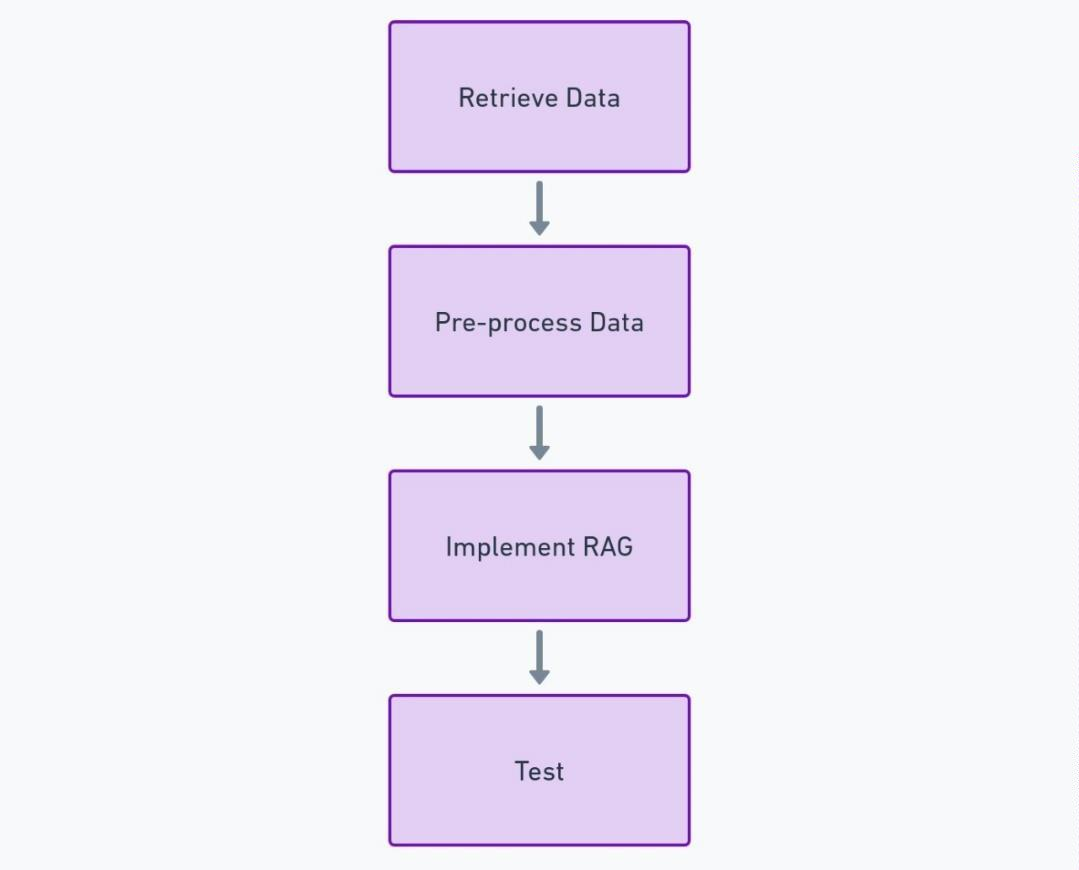
\includegraphics[width=352.35pt,height=284.03pt]{latexImage_1116eee783444c73f40b111da0dbc381.png}}
\end{picture}
\newpage
\begin{tikzpicture}[overlay]\path(0pt,0pt);\end{tikzpicture}
\begin{picture}(-5,0)(2.5,0)
\put(21.6,-35.35999){\fontsize{9.96}{1}\usefont{T1}{cmr}{m}{n}\selectfont\color{color_29791}  Breaking the Carbon Curve                                                                                                                                                  AY 2024-25 }
\end{picture}
\begin{tikzpicture}[overlay]
\path(0pt,0pt);
\filldraw[color_156561][even odd rule]
(20.16pt, -42.91998pt) -- (561.8199pt, -42.91998pt)
 -- (561.8199pt, -42.91998pt)
 -- (561.8199pt, -39.91998pt)
 -- (561.8199pt, -39.91998pt)
 -- (20.16pt, -39.91998pt) -- cycle
;
\filldraw[color_156561][even odd rule]
(20.16pt, -39.20001pt) -- (561.8199pt, -39.20001pt)
 -- (561.8199pt, -39.20001pt)
 -- (561.8199pt, -38.48004pt)
 -- (561.8199pt, -38.48004pt)
 -- (20.16pt, -38.48004pt) -- cycle
;
\end{tikzpicture}
\begin{picture}(-5,0)(2.5,0)
\put(291.05,-53.47998){\fontsize{11.04}{1}\usefont{T1}{cmr}{m}{n}\selectfont\color{color_29791} }
\put(21.6,-743.96){\fontsize{9.96}{1}\usefont{T1}{cmr}{m}{n}\selectfont\color{color_29791}     Dept. of CSE, DSCE                                                                                                                                                                          26 }
\end{picture}
\begin{tikzpicture}[overlay]
\path(0pt,0pt);
\filldraw[color_156561][even odd rule]
(20.16pt, -732.176pt) -- (568.92pt, -732.176pt)
 -- (568.92pt, -732.176pt)
 -- (568.92pt, -729.176pt)
 -- (568.92pt, -729.176pt)
 -- (20.16pt, -729.176pt) -- cycle
;
\filldraw[color_156561][even odd rule]
(20.16pt, -733.616pt) -- (568.92pt, -733.616pt)
 -- (568.92pt, -733.616pt)
 -- (568.92pt, -732.896pt)
 -- (568.92pt, -732.896pt)
 -- (20.16pt, -732.896pt) -- cycle
;
\end{tikzpicture}
\begin{picture}(-5,0)(2.5,0)
\put(57.024,-73.17999){\fontsize{12}{1}\usefont{T1}{cmr}{m}{n}\selectfont\color{color_29791} }
\put(57.024,-101.86){\fontsize{12}{1}\usefont{T1}{cmr}{m}{n}\selectfont\color{color_29791} }
\put(525.1,-324.01){\fontsize{12}{1}\usefont{T1}{cmr}{m}{n}\selectfont\color{color_29791} }
\put(192.17,-349.93){\fontsize{12}{1}\usefont{T1}{cmr}{m}{n}\selectfont\color{color_29791}Figure 4.4.4: Flowchart of RAG working }
\put(291.05,-378.61){\fontsize{12}{1}\usefont{T1}{cmr}{m}{n}\selectfont\color{color_29791} }
\put(57.024,-407.31){\fontsize{12}{1}\usefont{T1}{cmr}{m}{n}\selectfont\color{color_29791}3. Information Retrieval and Response Generation }
\put(84.504,-436.95){\fontsize{12}{1}\usefont{T1}{cmr}{m}{n}\selectfont\color{color_29791}• The system retrieves relevant data using FAISS and combines it with the user’s query.   }
\put(84.504,-458.55){\fontsize{12}{1}\usefont{T1}{cmr}{m}{n}\selectfont\color{color_29791}• The language model then generates a tailored response that includes emission calculations }
\put(102.5,-479.19){\fontsize{12}{1}\usefont{T1}{cmr}{m}{n}\selectfont\color{color_29791}and reduction strategies.   }
\put(102.5,-499.83){\fontsize{12}{1}\usefont{T1}{cmr}{m}{n}\selectfont\color{color_29791} }
\put(57.024,-528.51){\fontsize{12}{1}\usefont{T1}{cmr}{m}{n}\selectfont\color{color_29791}4. Output Display }
\put(84.504,-558.15){\fontsize{12}{1}\usefont{T1}{cmr}{m}{n}\selectfont\color{color_29791}• The assistant presents actionable suggestions through the Streamlit interface, making the }
\put(102.5,-578.82){\fontsize{12}{1}\usefont{T1}{cmr}{m}{n}\selectfont\color{color_29791}infor}
\put(57,-324){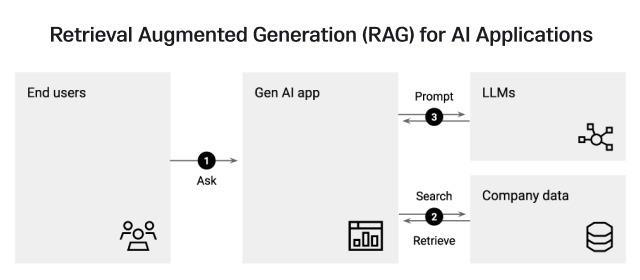
\includegraphics[width=468pt,height=204.6pt]{latexImage_b9085c07456a77628f86e4f6e9bde47c.png}}
\end{picture}
\newpage
\begin{tikzpicture}[overlay]\path(0pt,0pt);\end{tikzpicture}
\begin{picture}(-5,0)(2.5,0)
\put(21.6,-35.35999){\fontsize{9.96}{1}\usefont{T1}{cmr}{m}{n}\selectfont\color{color_29791}  Breaking the Carbon Curve                                                                                                                                                  AY 2024-25 }
\end{picture}
\begin{tikzpicture}[overlay]
\path(0pt,0pt);
\filldraw[color_156561][even odd rule]
(20.16pt, -42.91998pt) -- (561.8199pt, -42.91998pt)
 -- (561.8199pt, -42.91998pt)
 -- (561.8199pt, -39.91998pt)
 -- (561.8199pt, -39.91998pt)
 -- (20.16pt, -39.91998pt) -- cycle
;
\filldraw[color_156561][even odd rule]
(20.16pt, -39.20001pt) -- (561.8199pt, -39.20001pt)
 -- (561.8199pt, -39.20001pt)
 -- (561.8199pt, -38.48004pt)
 -- (561.8199pt, -38.48004pt)
 -- (20.16pt, -38.48004pt) -- cycle
;
\end{tikzpicture}
\begin{picture}(-5,0)(2.5,0)
\put(291.05,-53.47998){\fontsize{11.04}{1}\usefont{T1}{cmr}{m}{n}\selectfont\color{color_29791} }
\put(21.6,-743.96){\fontsize{9.96}{1}\usefont{T1}{cmr}{m}{n}\selectfont\color{color_29791}     Dept. of CSE, DSCE                                                                                                                                                                          27 }
\end{picture}
\begin{tikzpicture}[overlay]
\path(0pt,0pt);
\filldraw[color_156561][even odd rule]
(20.16pt, -732.176pt) -- (568.92pt, -732.176pt)
 -- (568.92pt, -732.176pt)
 -- (568.92pt, -729.176pt)
 -- (568.92pt, -729.176pt)
 -- (20.16pt, -729.176pt) -- cycle
;
\filldraw[color_156561][even odd rule]
(20.16pt, -733.616pt) -- (568.92pt, -733.616pt)
 -- (568.92pt, -733.616pt)
 -- (568.92pt, -732.896pt)
 -- (568.92pt, -732.896pt)
 -- (20.16pt, -732.896pt) -- cycle
;
\end{tikzpicture}
\begin{picture}(-5,0)(2.5,0)
\put(519.1,-305.05){\fontsize{12}{1}\usefont{T1}{cmr}{m}{n}\selectfont\color{color_29791} }
\put(175.73,-330.97){\fontsize{12}{1}\usefont{T1}{cmr}{m}{n}\selectfont\color{color_29791}Figure 4.4.5: User provided context and question to RAG  }
\put(57.024,-359.65){\fontsize{12}{1}\usefont{T1}{cmr}{m}{n}\selectfont\color{color_29791}In the figure 4.4.5, the information and questions provided are: }
\put(57.024,-388.33){\fontsize{12}{1}\usefont{T1}{cmr}{m}{n}\selectfont\color{color_29791}Context: I live in a two-bedroom apartment where I use an electric heater during winters for }
\put(57.024,-408.99){\fontsize{12}{1}\usefont{T1}{cmr}{m}{n}\selectfont\color{color_29791}about 5 hours a day. I work from home and use electronic devices (laptops, monitors, and a high-}
\put(57.024,-429.75){\fontsize{12}{1}\usefont{T1}{cmr}{m}{n}\selectfont\color{color_29791}end gaming desktop) for about 12 hours daily. For transportation, I rely on a hybrid vehicle for }
\put(57.024,-450.39){\fontsize{12}{1}\usefont{T1}{cmr}{m}{n}\selectfont\color{color_29791}short commutes (10-15 kilometres daily) and long trips twice a month. I regularly shop for }
\put(57.024,-471.15){\fontsize{12}{1}\usefont{T1}{cmr}{m}{n}\selectfont\color{color_29791}clothes online, averaging one or two purchases per month. I recycle plastics and paper but am }
\put(57.024,-491.79){\fontsize{12}{1}\usefont{T1}{cmr}{m}{n}\selectfont\color{color_29791}unsure about handling e-waste. }
\put(57.024,-520.47){\fontsize{12}{1}\usefont{T1}{cmr}{m}{n}\selectfont\color{color_29791}Question: Based on my lifestyle, can you provide a detailed analysis of my CO2 emissions and }
\put(57.024,-541.23){\fontsize{12}{1}\usefont{T1}{cmr}{m}{n}\selectfont\color{color_29791}suggest specific areas where I can make the most impactful reductions? }
\put(57.024,-569.19){\fontsize{11.04}{1}\usefont{T1}{cmr}{m}{n}\selectfont\color{color_29791} }
\put(57.024,-597.42){\fontsize{11.04}{1}\usefont{T1}{cmr}{m}{n}\selectfont\color{color_29791} }
\put(57.024,-625.5){\fontsize{11.04}{1}\usefont{T1}{cmr}{m}{n}\selectfont\color{color_29791} }
\put(57.024,-653.7){\fontsize{11.04}{1}\usefont{T1}{cmr}{m}{n}\selectfont\color{color_29791} }
\put(57,-305){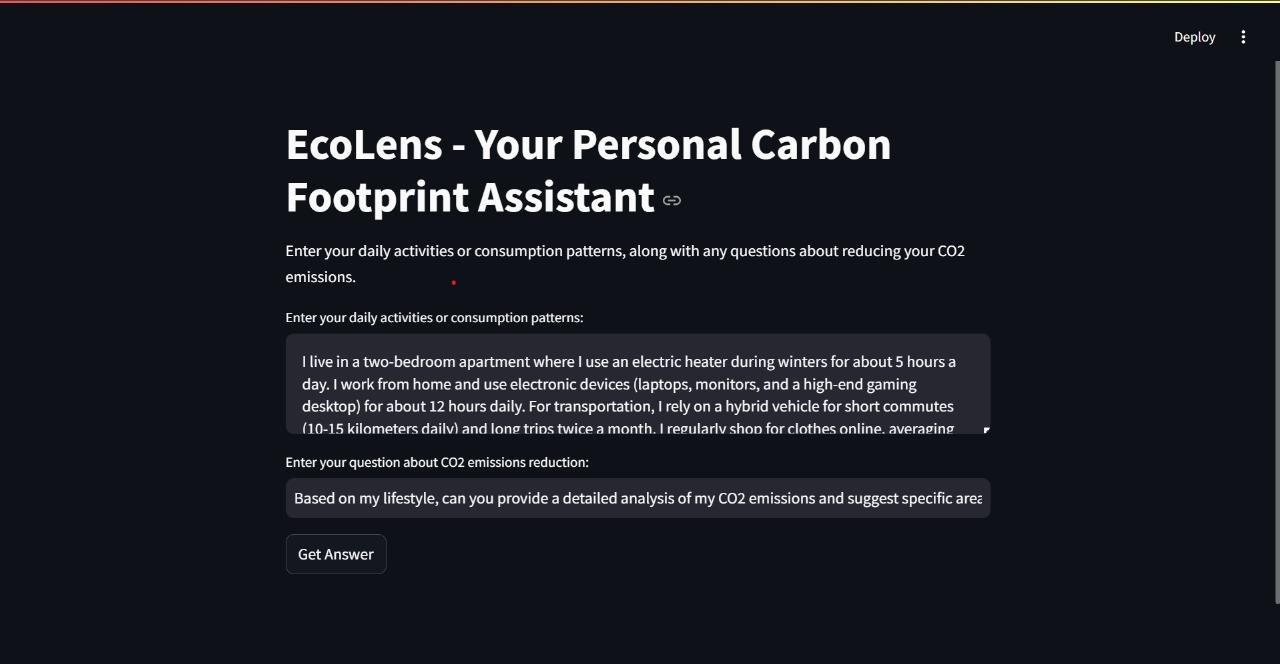
\includegraphics[width=461.5pt,height=243pt]{latexImage_08611834093e2b71e34222aa3fb333aa.png}}
\end{picture}
\newpage
\begin{tikzpicture}[overlay]\path(0pt,0pt);\end{tikzpicture}
\begin{picture}(-5,0)(2.5,0)
\put(21.6,-35.35999){\fontsize{9.96}{1}\usefont{T1}{cmr}{m}{n}\selectfont\color{color_29791}  Breaking the Carbon Curve                                                                                                                                                  AY 2024-25 }
\end{picture}
\begin{tikzpicture}[overlay]
\path(0pt,0pt);
\filldraw[color_156561][even odd rule]
(20.16pt, -42.91998pt) -- (561.8199pt, -42.91998pt)
 -- (561.8199pt, -42.91998pt)
 -- (561.8199pt, -39.91998pt)
 -- (561.8199pt, -39.91998pt)
 -- (20.16pt, -39.91998pt) -- cycle
;
\filldraw[color_156561][even odd rule]
(20.16pt, -39.20001pt) -- (561.8199pt, -39.20001pt)
 -- (561.8199pt, -39.20001pt)
 -- (561.8199pt, -38.48004pt)
 -- (561.8199pt, -38.48004pt)
 -- (20.16pt, -38.48004pt) -- cycle
;
\end{tikzpicture}
\begin{picture}(-5,0)(2.5,0)
\put(291.05,-53.47998){\fontsize{11.04}{1}\usefont{T1}{cmr}{m}{n}\selectfont\color{color_29791} }
\put(21.6,-743.96){\fontsize{9.96}{1}\usefont{T1}{cmr}{m}{n}\selectfont\color{color_29791}     Dept. of CSE, DSCE                                                                                                                                                                          28 }
\end{picture}
\begin{tikzpicture}[overlay]
\path(0pt,0pt);
\filldraw[color_156561][even odd rule]
(20.16pt, -732.176pt) -- (568.92pt, -732.176pt)
 -- (568.92pt, -732.176pt)
 -- (568.92pt, -729.176pt)
 -- (568.92pt, -729.176pt)
 -- (20.16pt, -729.176pt) -- cycle
;
\filldraw[color_156561][even odd rule]
(20.16pt, -733.616pt) -- (568.92pt, -733.616pt)
 -- (568.92pt, -733.616pt)
 -- (568.92pt, -732.896pt)
 -- (568.92pt, -732.896pt)
 -- (20.16pt, -732.896pt) -- cycle
;
\end{tikzpicture}
\begin{picture}(-5,0)(2.5,0)
\put(525.1,-305.05){\fontsize{12}{1}\usefont{T1}{cmr}{m}{n}\selectfont\color{color_29791} }
\put(148.7,-330.97){\fontsize{12}{1}\usefont{T1}{cmr}{m}{n}\selectfont\color{color_29791}Figure 4.4.6: Calculation part of ecolens on CO2 emissions }
\put(525.1,-587.1){\fontsize{12}{1}\usefont{T1}{cmr}{m}{n}\selectfont\color{color_29791} }
\put(183.77,-612.9){\fontsize{12}{1}\usefont{T1}{cmr}{m}{n}\selectfont\color{color_29791}Figure 4.4.7: Recommendations and insights }
\put(291.05,-633.54){\fontsize{12}{1}\usefont{T1}{cmr}{m}{n}\selectfont\color{color_29791} }
\put(291.05,-662.34){\fontsize{12}{1}\usefont{T1}{cmr}{m}{n}\selectfont\color{color_29791} }
\put(291.05,-691.016){\fontsize{12}{1}\usefont{T1}{cmr}{m}{n}\selectfont\color{color_29791} }
\put(57,-304.35){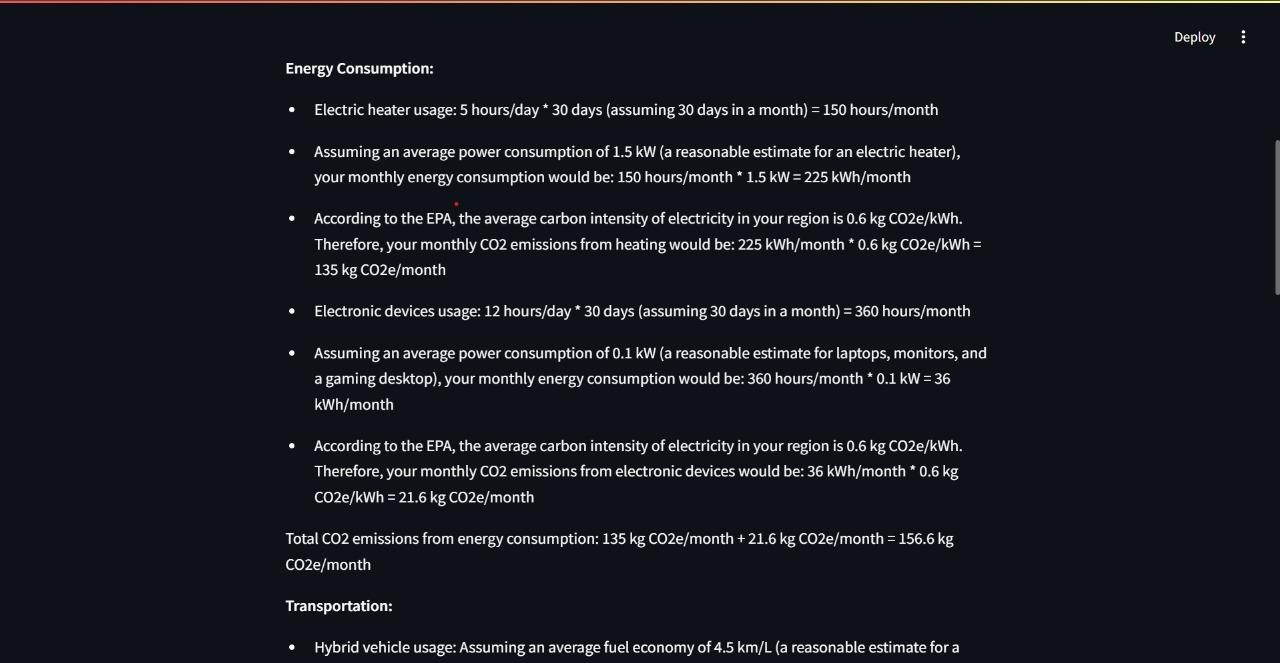
\includegraphics[width=468pt,height=242.35pt]{latexImage_95dec6f7c408bbce816faa41c62ce0b6.png}}
\put(57,-586.36){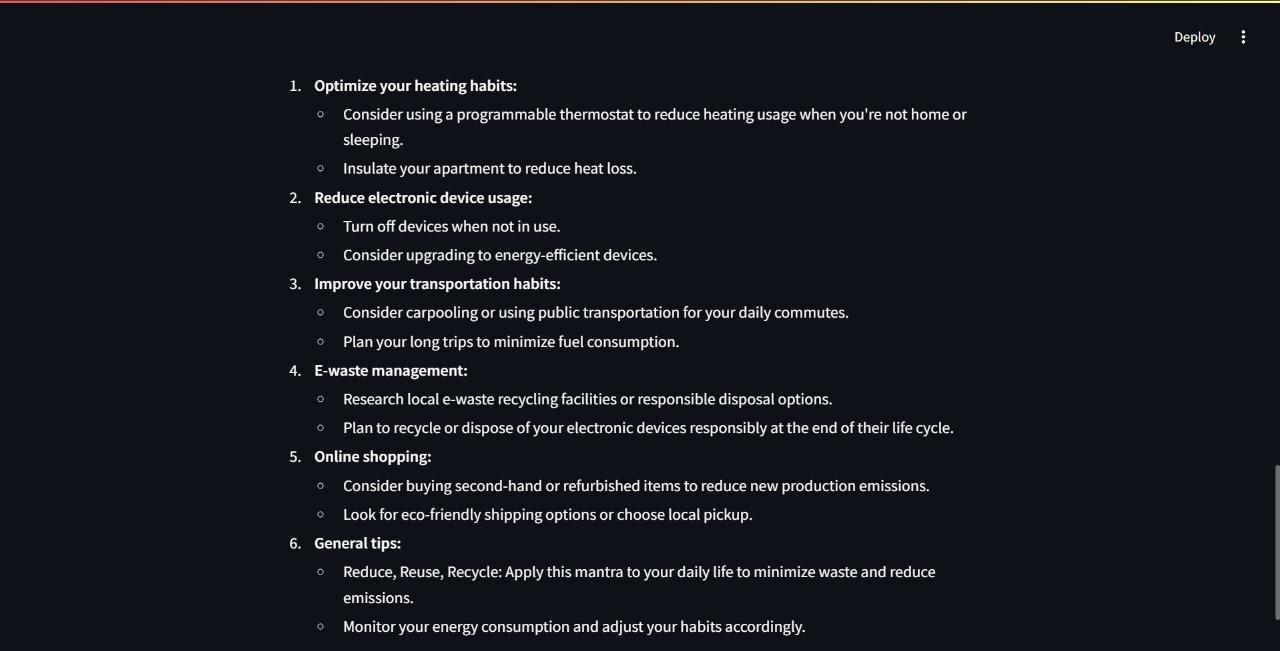
\includegraphics[width=468pt,height=237.95pt]{latexImage_bcd3e4c85121cba74ea1aa3d02ad1bec.png}}
\end{picture}
\newpage
\begin{tikzpicture}[overlay]\path(0pt,0pt);\end{tikzpicture}
\begin{picture}(-5,0)(2.5,0)
\put(21.6,-35.35999){\fontsize{9.96}{1}\usefont{T1}{cmr}{m}{n}\selectfont\color{color_29791}  Breaking the Carbon Curve                                                                                                                                                  AY 2024-25 }
\end{picture}
\begin{tikzpicture}[overlay]
\path(0pt,0pt);
\filldraw[color_156561][even odd rule]
(20.16pt, -42.91998pt) -- (561.8199pt, -42.91998pt)
 -- (561.8199pt, -42.91998pt)
 -- (561.8199pt, -39.91998pt)
 -- (561.8199pt, -39.91998pt)
 -- (20.16pt, -39.91998pt) -- cycle
;
\filldraw[color_156561][even odd rule]
(20.16pt, -39.20001pt) -- (561.8199pt, -39.20001pt)
 -- (561.8199pt, -39.20001pt)
 -- (561.8199pt, -38.48004pt)
 -- (561.8199pt, -38.48004pt)
 -- (20.16pt, -38.48004pt) -- cycle
;
\end{tikzpicture}
\begin{picture}(-5,0)(2.5,0)
\put(291.05,-53.47998){\fontsize{11.04}{1}\usefont{T1}{cmr}{m}{n}\selectfont\color{color_29791} }
\put(21.6,-743.96){\fontsize{9.96}{1}\usefont{T1}{cmr}{m}{n}\selectfont\color{color_29791}     Dept. of CSE, DSCE                                                                                                                                                                          29 }
\end{picture}
\begin{tikzpicture}[overlay]
\path(0pt,0pt);
\filldraw[color_156561][even odd rule]
(20.16pt, -732.176pt) -- (568.92pt, -732.176pt)
 -- (568.92pt, -732.176pt)
 -- (568.92pt, -729.176pt)
 -- (568.92pt, -729.176pt)
 -- (20.16pt, -729.176pt) -- cycle
;
\filldraw[color_156561][even odd rule]
(20.16pt, -733.616pt) -- (568.92pt, -733.616pt)
 -- (568.92pt, -733.616pt)
 -- (568.92pt, -732.896pt)
 -- (568.92pt, -732.896pt)
 -- (20.16pt, -732.896pt) -- cycle
;
\end{tikzpicture}
\begin{picture}(-5,0)(2.5,0)
\put(57.024,-73.17999){\fontsize{12}{1}\usefont{T1}{cmr}{m}{n}\selectfont\color{color_29791}How This Enhances the Project - }
\put(75.024,-102.82){\fontsize{12}{1}\usefont{T1}{cmr}{m}{n}\selectfont\color{color_29791}• The CO2 Emissions Assistant empowers individuals to better understand the impact of }
\put(93.02,-123.46){\fontsize{12}{1}\usefont{T1}{cmr}{m}{n}\selectfont\color{color_29791}their daily activities on the environment. It bridges the gap between large-scale data }
\put(93.02,-144.1){\fontsize{12}{1}\usefont{T1}{cmr}{m}{n}\selectfont\color{color_29791}analysis and personal action by providing tailored insights. This complements the project’s }
\put(93.02,-164.86){\fontsize{12}{1}\usefont{T1}{cmr}{m}{n}\selectfont\color{color_29791}forecasting tools, which address broader emission trends, by offering solutions at an }
\put(93.02,-185.5){\fontsize{12}{1}\usefont{T1}{cmr}{m}{n}\selectfont\color{color_29791}individual level. It also aligns personal behavior with global sustainability goals, }
\put(93.02,-206.26){\fontsize{12}{1}\usefont{T1}{cmr}{m}{n}\selectfont\color{color_29791}demonstrating the potential of AI in driving meaningful climate action. }
\put(93.02,-226.9){\fontsize{12}{1}\usefont{T1}{cmr}{m}{n}\selectfont\color{color_29791} }
\put(57.024,-255.61){\fontsize{12}{1}\usefont{T1}{cmr}{m}{n}\selectfont\color{color_29791}The LLM-Powered CO2 Emissions Assistant is a practical addition to the project, focusing on }
\put(57.024,-276.37){\fontsize{12}{1}\usefont{T1}{cmr}{m}{n}\selectfont\color{color_29791}individual empowerment through personalized insights. By integrating advanced AI technologies }
\put(57.024,-297.01){\fontsize{12}{1}\usefont{T1}{cmr}{m}{n}\selectfont\color{color_29791}with user-friendly tools, it enhances the project’s reach and impact, showing how AI can be }
\put(57.024,-317.77){\fontsize{12}{1}\usefont{T1}{cmr}{m}{n}\selectfont\color{color_29791}harnessed to promote sustainability and encourage climate-conscious actions. }
\put(57.024,-346.45){\fontsize{12}{1}\usefont{T1}{cmr}{m}{n}\selectfont\color{color_29791} }
\put(57.024,-375.13){\fontsize{12}{1}\usefont{T1}{cmr}{m}{n}\selectfont\color{color_29791} }
\put(57.024,-407.67){\fontsize{15.96}{1}\usefont{T1}{cmr}{m}{n}\selectfont\color{color_29791}4.5 Algorithms }
\put(57.024,-439.47){\fontsize{12}{1}\usefont{T1}{cmr}{m}{n}\selectfont\color{color_29791}1. ARIMA (Autoregressive Integrated Moving Average) }
\put(75.024,-468.15){\fontsize{9.96}{1}\usefont{T1}{cmr}{m}{n}\selectfont\color{color_29791}• Step 1: Test for stationarity using ADF or KPSS tests. }
\put(75.024,-496.83){\fontsize{9.96}{1}\usefont{T1}{cmr}{m}{n}\selectfont\color{color_29791}• Step 2: Analyse ACF and PACF plots to determine the parameters ppp, ddd, and qqq. }
\put(75.024,-525.51){\fontsize{9.96}{1}\usefont{T1}{cmr}{m}{n}\selectfont\color{color_29791}• Step 3: Fit the ARIMA model to the time-series data. }
\put(75.024,-554.31){\fontsize{9.96}{1}\usefont{T1}{cmr}{m}{n}\selectfont\color{color_29791}• Step 4: Evaluate the model using metrics like MSE, RMSE, and MAE. }
\put(75.024,-583.02){\fontsize{9.96}{1}\usefont{T1}{cmr}{m}{n}\selectfont\color{color_29791}• Step 5: Use the model for short- or long-term forecasts. }
\end{picture}
\newpage
\begin{tikzpicture}[overlay]\path(0pt,0pt);\end{tikzpicture}
\begin{picture}(-5,0)(2.5,0)
\put(21.6,-35.35999){\fontsize{9.96}{1}\usefont{T1}{cmr}{m}{n}\selectfont\color{color_29791}  Breaking the Carbon Curve                                                                                                                                                  AY 2024-25 }
\end{picture}
\begin{tikzpicture}[overlay]
\path(0pt,0pt);
\filldraw[color_156561][even odd rule]
(20.16pt, -42.91998pt) -- (561.8199pt, -42.91998pt)
 -- (561.8199pt, -42.91998pt)
 -- (561.8199pt, -39.91998pt)
 -- (561.8199pt, -39.91998pt)
 -- (20.16pt, -39.91998pt) -- cycle
;
\filldraw[color_156561][even odd rule]
(20.16pt, -39.20001pt) -- (561.8199pt, -39.20001pt)
 -- (561.8199pt, -39.20001pt)
 -- (561.8199pt, -38.48004pt)
 -- (561.8199pt, -38.48004pt)
 -- (20.16pt, -38.48004pt) -- cycle
;
\end{tikzpicture}
\begin{picture}(-5,0)(2.5,0)
\put(291.05,-53.47998){\fontsize{11.04}{1}\usefont{T1}{cmr}{m}{n}\selectfont\color{color_29791} }
\put(21.6,-743.96){\fontsize{9.96}{1}\usefont{T1}{cmr}{m}{n}\selectfont\color{color_29791}     Dept. of CSE, DSCE                                                                                                                                                                          30 }
\end{picture}
\begin{tikzpicture}[overlay]
\path(0pt,0pt);
\filldraw[color_156561][even odd rule]
(20.16pt, -732.176pt) -- (568.92pt, -732.176pt)
 -- (568.92pt, -732.176pt)
 -- (568.92pt, -729.176pt)
 -- (568.92pt, -729.176pt)
 -- (20.16pt, -729.176pt) -- cycle
;
\filldraw[color_156561][even odd rule]
(20.16pt, -733.616pt) -- (568.92pt, -733.616pt)
 -- (568.92pt, -733.616pt)
 -- (568.92pt, -732.896pt)
 -- (568.92pt, -732.896pt)
 -- (20.16pt, -732.896pt) -- cycle
;
\end{tikzpicture}
\begin{picture}(-5,0)(2.5,0)
\put(525.1,-354.61){\fontsize{12}{1}\usefont{T1}{cmr}{m}{n}\selectfont\color{color_29791} }
\put(198.65,-380.41){\fontsize{12}{1}\usefont{T1}{cmr}{m}{n}\selectfont\color{color_29791}Figure 4.2.1: Arima model prediction od CO2 }
\put(309.07,-409.11){\fontsize{12}{1}\usefont{T1}{cmr}{m}{n}\selectfont\color{color_29791} }
\put(309.07,-437.79){\fontsize{12}{1}\usefont{T1}{cmr}{m}{n}\selectfont\color{color_29791} }
\put(57.024,-466.59){\fontsize{12}{1}\usefont{T1}{cmr}{m}{n}\selectfont\color{color_29791}2. CNN-GRU Algorithm }
\put(75.024,-495.27){\fontsize{9.96}{1}\usefont{T1}{cmr}{m}{n}\selectfont\color{color_29791}• Step 1: Preprocess the data into overlapping input-output sequences. }
\put(75.024,-523.95){\fontsize{9.96}{1}\usefont{T1}{cmr}{m}{n}\selectfont\color{color_29791}• Step 2: Use CNN layers to extract meaningful patterns from the sequences. }
\put(75.024,-552.63){\fontsize{9.96}{1}\usefont{T1}{cmr}{m}{n}\selectfont\color{color_29791}• Step 3: Pass the extracted features into GRU layers to learn temporal dependencies. }
\put(75.024,-581.34){\fontsize{9.96}{1}\usefont{T1}{cmr}{m}{n}\selectfont\color{color_29791}• Step 4: Add dense layers for final output predictions. }
\put(75.024,-610.02){\fontsize{9.96}{1}\usefont{T1}{cmr}{m}{n}\selectfont\color{color_29791}•}
\put(57,-354.35){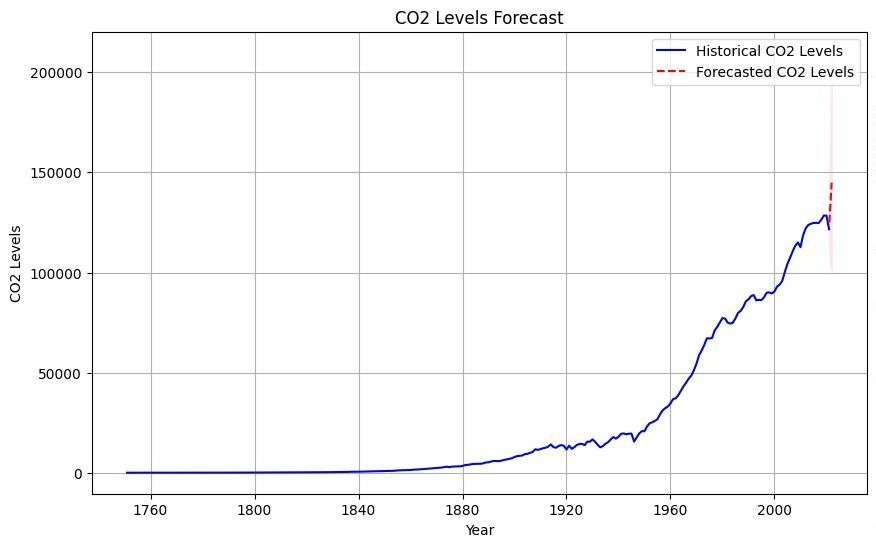
\includegraphics[width=468pt,height=292.35pt]{latexImage_61312e2e7ba485a296f072772c2fc0d9.png}}
\end{picture}
\newpage
\begin{tikzpicture}[overlay]\path(0pt,0pt);\end{tikzpicture}
\begin{picture}(-5,0)(2.5,0)
\put(21.6,-35.35999){\fontsize{9.96}{1}\usefont{T1}{cmr}{m}{n}\selectfont\color{color_29791}  Breaking the Carbon Curve                                                                                                                                                  AY 2024-25 }
\end{picture}
\begin{tikzpicture}[overlay]
\path(0pt,0pt);
\filldraw[color_156561][even odd rule]
(20.16pt, -42.91998pt) -- (561.8199pt, -42.91998pt)
 -- (561.8199pt, -42.91998pt)
 -- (561.8199pt, -39.91998pt)
 -- (561.8199pt, -39.91998pt)
 -- (20.16pt, -39.91998pt) -- cycle
;
\filldraw[color_156561][even odd rule]
(20.16pt, -39.20001pt) -- (561.8199pt, -39.20001pt)
 -- (561.8199pt, -39.20001pt)
 -- (561.8199pt, -38.48004pt)
 -- (561.8199pt, -38.48004pt)
 -- (20.16pt, -38.48004pt) -- cycle
;
\end{tikzpicture}
\begin{picture}(-5,0)(2.5,0)
\put(291.05,-53.47998){\fontsize{11.04}{1}\usefont{T1}{cmr}{m}{n}\selectfont\color{color_29791} }
\put(21.6,-743.96){\fontsize{9.96}{1}\usefont{T1}{cmr}{m}{n}\selectfont\color{color_29791}     Dept. of CSE, DSCE                                                                                                                                                                          31 }
\end{picture}
\begin{tikzpicture}[overlay]
\path(0pt,0pt);
\filldraw[color_156561][even odd rule]
(20.16pt, -732.176pt) -- (568.92pt, -732.176pt)
 -- (568.92pt, -732.176pt)
 -- (568.92pt, -729.176pt)
 -- (568.92pt, -729.176pt)
 -- (20.16pt, -729.176pt) -- cycle
;
\filldraw[color_156561][even odd rule]
(20.16pt, -733.616pt) -- (568.92pt, -733.616pt)
 -- (568.92pt, -733.616pt)
 -- (568.92pt, -732.896pt)
 -- (568.92pt, -732.896pt)
 -- (20.16pt, -732.896pt) -- cycle
;
\end{tikzpicture}
\begin{picture}(-5,0)(2.5,0)
\put(561.1,-342.85){\fontsize{12}{1}\usefont{T1}{cmr}{m}{n}\selectfont\color{color_29791} }
\put(187.61,-368.77){\fontsize{12}{1}\usefont{T1}{cmr}{m}{n}\selectfont\color{color_29791}Figure 4.2.2: CNN-GRU model prediction of CO2 }
\put(309.07,-397.45){\fontsize{12}{1}\usefont{T1}{cmr}{m}{n}\selectfont\color{color_29791} }
\put(309.07,-426.15){\fontsize{12}{1}\usefont{T1}{cmr}{m}{n}\selectfont\color{color_29791} }
\put(57.024,-454.83){\fontsize{12}{1}\usefont{T1}{cmr}{m}{n}\selectfont\color{color_29791}3. CNN-LSTM Algorithm }
\put(75.024,-483.51){\fontsize{9.96}{1}\usefont{T1}{cmr}{m}{n}\selectfont\color{color_29791}• Step 1: Prepare time-series data similarly to CNN-GRU. }
\put(75.024,-512.19){\fontsize{9.96}{1}\usefont{T1}{cmr}{m}{n}\selectfont\color{color_29791}• Step 2: Use CNN layers to detect patterns in the input data. }
\put(75.024,-540.99){\fontsize{9.96}{1}\usefont{T1}{cmr}{m}{n}\selectfont\color{color_29791}• Step 3: Feed the CNN outputs into LSTM layers to learn long-term dependencies. }
\put(75.024,-569.67){\fontsize{9.96}{1}\usefont{T1}{cmr}{m}{n}\selectfont\color{color_29791}• Step 4: Add fully connected layers for making predictions. }
\put(75.024,-598.38){\fontsize{9.96}{1}\usefont{T1}{cmr}{m}{n}\selectfont\color{color_29791}•}
\put(93,-342.8){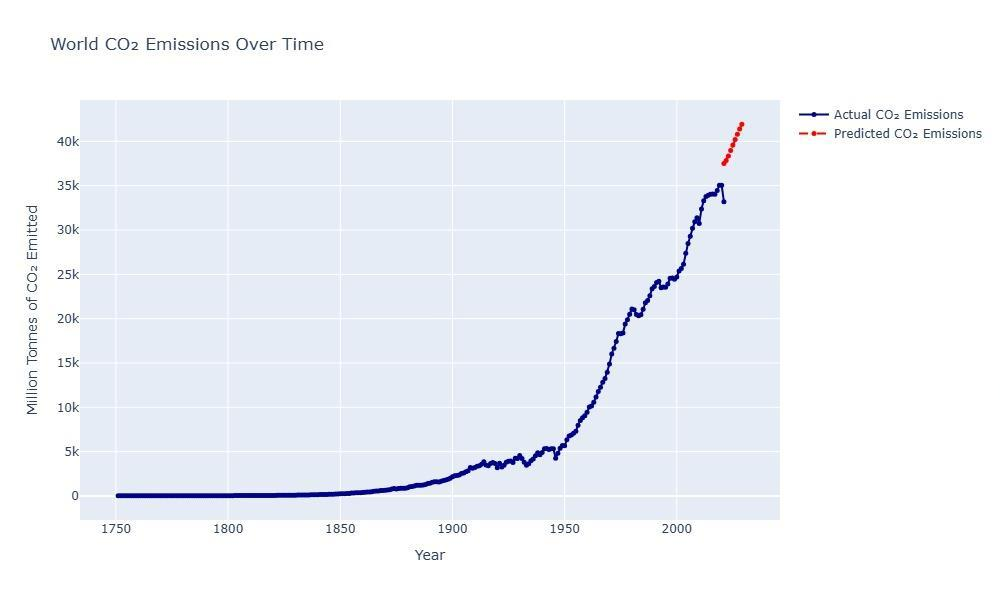
\includegraphics[width=468pt,height=280.8pt]{latexImage_0683f305f4267601f72af31bfd36be35.png}}
\end{picture}
\newpage
\begin{tikzpicture}[overlay]\path(0pt,0pt);\end{tikzpicture}
\begin{picture}(-5,0)(2.5,0)
\put(21.6,-35.35999){\fontsize{9.96}{1}\usefont{T1}{cmr}{m}{n}\selectfont\color{color_29791}  Breaking the Carbon Curve                                                                                                                                                  AY 2024-25 }
\end{picture}
\begin{tikzpicture}[overlay]
\path(0pt,0pt);
\filldraw[color_156561][even odd rule]
(20.16pt, -42.91998pt) -- (561.8199pt, -42.91998pt)
 -- (561.8199pt, -42.91998pt)
 -- (561.8199pt, -39.91998pt)
 -- (561.8199pt, -39.91998pt)
 -- (20.16pt, -39.91998pt) -- cycle
;
\filldraw[color_156561][even odd rule]
(20.16pt, -39.20001pt) -- (561.8199pt, -39.20001pt)
 -- (561.8199pt, -39.20001pt)
 -- (561.8199pt, -38.48004pt)
 -- (561.8199pt, -38.48004pt)
 -- (20.16pt, -38.48004pt) -- cycle
;
\end{tikzpicture}
\begin{picture}(-5,0)(2.5,0)
\put(291.05,-53.47998){\fontsize{11.04}{1}\usefont{T1}{cmr}{m}{n}\selectfont\color{color_29791} }
\put(21.6,-743.96){\fontsize{9.96}{1}\usefont{T1}{cmr}{m}{n}\selectfont\color{color_29791}     Dept. of CSE, DSCE                                                                                                                                                                          32 }
\end{picture}
\begin{tikzpicture}[overlay]
\path(0pt,0pt);
\filldraw[color_156561][even odd rule]
(20.16pt, -732.176pt) -- (568.92pt, -732.176pt)
 -- (568.92pt, -732.176pt)
 -- (568.92pt, -729.176pt)
 -- (568.92pt, -729.176pt)
 -- (20.16pt, -729.176pt) -- cycle
;
\filldraw[color_156561][even odd rule]
(20.16pt, -733.616pt) -- (568.92pt, -733.616pt)
 -- (568.92pt, -733.616pt)
 -- (568.92pt, -732.896pt)
 -- (568.92pt, -732.896pt)
 -- (20.16pt, -732.896pt) -- cycle
;
\end{tikzpicture}
\begin{picture}(-5,0)(2.5,0)
\put(582.48,-312.61){\fontsize{12}{1}\usefont{T1}{cmr}{m}{n}\selectfont\color{color_29791} }
\put(184.37,-338.41){\fontsize{12}{1}\usefont{T1}{cmr}{m}{n}\selectfont\color{color_29791}Figure 4.2.3: CNN-LSTM model prediction of CO2 }
\put(57.024,-367.09){\fontsize{12}{1}\usefont{T1}{cmr}{m}{n}\selectfont\color{color_29791}4. LSTM Model }
\put(75.024,-395.77){\fontsize{9.96}{1}\usefont{T1}{cmr}{m}{n}\selectfont\color{color_29791}• Step 1: Preprocess the data by normalizing values and segmenting the time series into }
\put(93.02,-416.55){\fontsize{12}{1}\usefont{T1}{cmr}{m}{n}\selectfont\color{color_29791}input-output sequences for training. }
\put(75.024,-445.23){\fontsize{9.96}{1}\usefont{T1}{cmr}{m}{n}\selectfont\color{color_29791}• Step 2: Build an LSTM network with one or more LSTM layers, each containing a }
\put(93.02,-465.99){\fontsize{12}{1}\usefont{T1}{cmr}{m}{n}\selectfont\color{color_29791}specified number of units to capture temporal dependencies. }
\put(75.024,-494.67){\fontsize{9.96}{1}\usefont{T1}{cmr}{m}{n}\selectfont\color{color_29791}• Step 3: Add dropout layers to prevent overfitting and dense layers to generate the final }
\put(93.02,-515.31){\fontsize{12}{1}\usefont{T1}{cmr}{m}{n}\selectfont\color{color_29791}output predictions. }
\put(75.024,-543.99){\fontsize{9.96}{1}\usefont{T1}{cmr}{m}{n}\selectfont\color{color_29791}• Step 4: Compile the model using an optimizer like Adam and a loss function such as Mean }
\put(93.02,-564.75){\fontsize{12}{1}\usefont{T1}{cmr}{m}{n}\selectfont\color{color_29791}Squared Error. }
\put(75.024,-593.46){\fontsize{9.96}{1}\usefont{T1}{cmr}{m}{n}\selectfont\color{color_29791}• Step 5: Train the model on the training dataset while monitoring performance metrics like }
\put(93.02,-614.1){\fontsize{12}{1}\usefont{T1}{cmr}{m}{n}\selectfont\color{color_29791}RMSE and MAE for validation. }
\put(75.024,-642.9){\fontsize{9.96}{1}\usefont{T1}{cmr}{m}{n}\selectfont\color{color_29791}• Step 6: Use the trained model for forecasting, adjusting the sequence length and tuning the }
\put(93.02,-663.54){\fontsize{12}{1}\usefont{T1}{cmr}{m}{n}\selectfont\color{color_29791}model f}
\put(57,-312.28){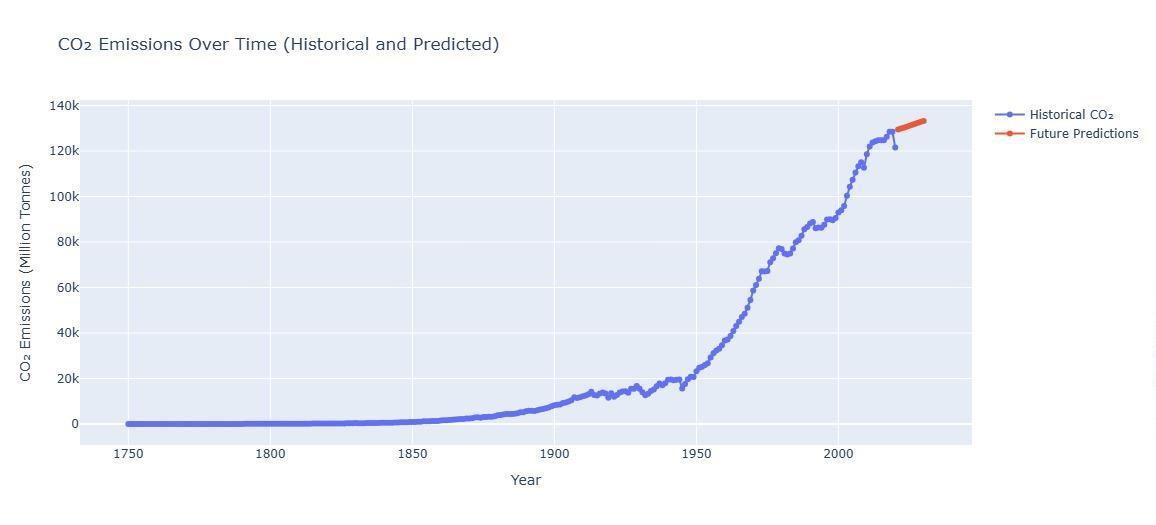
\includegraphics[width=525.45pt,height=250.28pt]{latexImage_976dccaf570c8d470a9dd1f4895c4621.png}}
\end{picture}
\newpage
\begin{tikzpicture}[overlay]\path(0pt,0pt);\end{tikzpicture}
\begin{picture}(-5,0)(2.5,0)
\put(21.6,-35.35999){\fontsize{9.96}{1}\usefont{T1}{cmr}{m}{n}\selectfont\color{color_29791}  Breaking the Carbon Curve                                                                                                                                                  AY 2024-25 }
\end{picture}
\begin{tikzpicture}[overlay]
\path(0pt,0pt);
\filldraw[color_156561][even odd rule]
(20.16pt, -42.91998pt) -- (561.8199pt, -42.91998pt)
 -- (561.8199pt, -42.91998pt)
 -- (561.8199pt, -39.91998pt)
 -- (561.8199pt, -39.91998pt)
 -- (20.16pt, -39.91998pt) -- cycle
;
\filldraw[color_156561][even odd rule]
(20.16pt, -39.20001pt) -- (561.8199pt, -39.20001pt)
 -- (561.8199pt, -39.20001pt)
 -- (561.8199pt, -38.48004pt)
 -- (561.8199pt, -38.48004pt)
 -- (20.16pt, -38.48004pt) -- cycle
;
\end{tikzpicture}
\begin{picture}(-5,0)(2.5,0)
\put(291.05,-53.47998){\fontsize{11.04}{1}\usefont{T1}{cmr}{m}{n}\selectfont\color{color_29791} }
\put(21.6,-743.96){\fontsize{9.96}{1}\usefont{T1}{cmr}{m}{n}\selectfont\color{color_29791}     Dept. of CSE, DSCE                                                                                                                                                                          33 }
\end{picture}
\begin{tikzpicture}[overlay]
\path(0pt,0pt);
\filldraw[color_156561][even odd rule]
(20.16pt, -732.176pt) -- (568.92pt, -732.176pt)
 -- (568.92pt, -732.176pt)
 -- (568.92pt, -729.176pt)
 -- (568.92pt, -729.176pt)
 -- (20.16pt, -729.176pt) -- cycle
;
\filldraw[color_156561][even odd rule]
(20.16pt, -733.616pt) -- (568.92pt, -733.616pt)
 -- (568.92pt, -733.616pt)
 -- (568.92pt, -732.896pt)
 -- (568.92pt, -732.896pt)
 -- (20.16pt, -732.896pt) -- cycle
;
\end{tikzpicture}
\begin{picture}(-5,0)(2.5,0)
\put(520.54,-293.05){\fontsize{12}{1}\usefont{T1}{cmr}{m}{n}\selectfont\color{color_29791} }
\put(218.33,-318.97){\fontsize{12}{1}\usefont{T1}{cmr}{m}{n}\selectfont\color{color_29791}Figure 4.2.4: LSTM model prediction }
\put(309.07,-347.65){\fontsize{12}{1}\usefont{T1}{cmr}{m}{n}\selectfont\color{color_29791} }
\put(57.024,-376.33){\fontsize{12}{1}\usefont{T1}{cmr}{m}{n}\selectfont\color{color_29791} }
\put(57.024,-405.03){\fontsize{12}{1}\usefont{T1}{cmr}{m}{n}\selectfont\color{color_29791} }
\put(57.024,-433.71){\fontsize{12}{1}\usefont{T1}{cmr}{m}{n}\selectfont\color{color_29791} }
\put(57.024,-462.39){\fontsize{12}{1}\usefont{T1}{cmr}{m}{n}\selectfont\color{color_29791} }
\put(57.024,-491.19){\fontsize{12}{1}\usefont{T1}{cmr}{m}{n}\selectfont\color{color_29791} }
\put(57.024,-519.87){\fontsize{12}{1}\usefont{T1}{cmr}{m}{n}\selectfont\color{color_29791} }
\put(57.024,-548.55){\fontsize{12}{1}\usefont{T1}{cmr}{m}{n}\selectfont\color{color_29791} }
\put(57.024,-577.26){\fontsize{12}{1}\usefont{T1}{cmr}{m}{n}\selectfont\color{color_29791} }
\put(57.024,-605.94){\fontsize{12}{1}\usefont{T1}{cmr}{m}{n}\selectfont\color{color_29791} }
\put(57.024,-634.62){\fontsize{12}{1}\usefont{T1}{cmr}{m}{n}\selectfont\color{color_29791} }
\put(57.024,-663.3){\fontsize{12}{1}\usefont{T1}{cmr}{m}{n}\selectfont\color{color_29791} }
\put(57.024,-692.096){\fontsize{12}{1}\usefont{T1}{cmr}{m}{n}\selectfont\color{color_29791} }
\put(97.5,-292.7){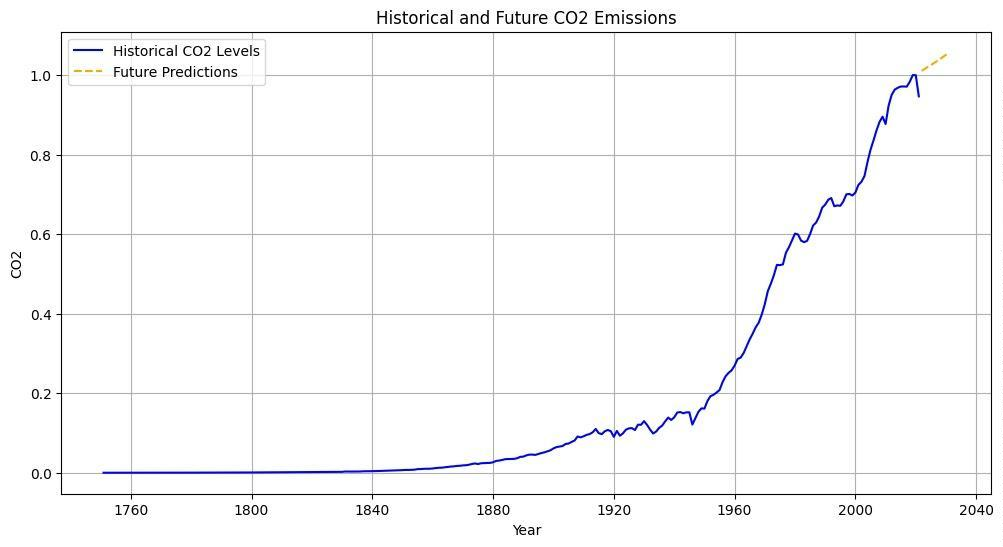
\includegraphics[width=422.99pt,height=230.7pt]{latexImage_ddf361de6d91382faeaab2a9f6ef8178.png}}
\end{picture}
\newpage
\begin{tikzpicture}[overlay]\path(0pt,0pt);\end{tikzpicture}
\begin{picture}(-5,0)(2.5,0)
\put(21.6,-35.35999){\fontsize{9.96}{1}\usefont{T1}{cmr}{m}{n}\selectfont\color{color_29791}  Breaking the Carbon Curve                                                                                                                                                  AY 2024-25 }
\end{picture}
\begin{tikzpicture}[overlay]
\path(0pt,0pt);
\filldraw[color_156561][even odd rule]
(20.16pt, -42.91998pt) -- (561.8199pt, -42.91998pt)
 -- (561.8199pt, -42.91998pt)
 -- (561.8199pt, -39.91998pt)
 -- (561.8199pt, -39.91998pt)
 -- (20.16pt, -39.91998pt) -- cycle
;
\filldraw[color_156561][even odd rule]
(20.16pt, -39.20001pt) -- (561.8199pt, -39.20001pt)
 -- (561.8199pt, -39.20001pt)
 -- (561.8199pt, -38.48004pt)
 -- (561.8199pt, -38.48004pt)
 -- (20.16pt, -38.48004pt) -- cycle
;
\end{tikzpicture}
\begin{picture}(-5,0)(2.5,0)
\put(291.05,-53.47998){\fontsize{11.04}{1}\usefont{T1}{cmr}{m}{n}\selectfont\color{color_29791} }
\put(21.6,-743.96){\fontsize{9.96}{1}\usefont{T1}{cmr}{m}{n}\selectfont\color{color_29791}     Dept. of CSE, DSCE                                                                                                                                                                          34 }
\end{picture}
\begin{tikzpicture}[overlay]
\path(0pt,0pt);
\filldraw[color_156561][even odd rule]
(20.16pt, -732.176pt) -- (568.92pt, -732.176pt)
 -- (568.92pt, -732.176pt)
 -- (568.92pt, -729.176pt)
 -- (568.92pt, -729.176pt)
 -- (20.16pt, -729.176pt) -- cycle
;
\filldraw[color_156561][even odd rule]
(20.16pt, -733.616pt) -- (568.92pt, -733.616pt)
 -- (568.92pt, -733.616pt)
 -- (568.92pt, -732.896pt)
 -- (568.92pt, -732.896pt)
 -- (20.16pt, -732.896pt) -- cycle
;
\end{tikzpicture}
\begin{picture}(-5,0)(2.5,0)
\put(57.024,-80.73999){\fontsize{20.04}{1}\usefont{T1}{cmr}{m}{n}\selectfont\color{color_29791}Chapter 5 }
\put(262.49,-111.58){\fontsize{18}{1}\usefont{T1}{cmr}{m}{n}\selectfont\color{color_29791}Testing }
\put(57.024,-148.9){\fontsize{15.96}{1}\usefont{T1}{cmr}{m}{n}\selectfont\color{color_29791}5.1 Unit Testing }
\put(57.024,-180.7){\fontsize{12}{1}\usefont{T1}{cmr}{m}{n}\selectfont\color{color_29791}Unit testing checks the functionality of individual components in the system to ensure they perform }
\put(57.024,-201.34){\fontsize{12}{1}\usefont{T1}{cmr}{m}{n}\selectfont\color{color_29791}as expected. The following are the key test cases for each module: }
\put(57.024,-230.02){\fontsize{12}{1}\usefont{T1}{cmr}{m}{n}\selectfont\color{color_29791}1. Data Preprocessing Module }
\put(75.024,-258.73){\fontsize{9.96}{1}\usefont{T1}{cmr}{m}{n}\selectfont\color{color_29791}• Test Case 1: Handling Missing Values }
\put(111.02,-287.41){\fontsize{9.96}{1}\usefont{T1}{cmr}{m}{n}\selectfont\color{color_29791}o Description: Ensure that missing data is correctly filled or replaced using }
\put(129.02,-308.17){\fontsize{12}{1}\usefont{T1}{cmr}{m}{n}\selectfont\color{color_29791}techniques like mean or median imputation. }
\put(111.02,-336.85){\fontsize{9.96}{1}\usefont{T1}{cmr}{m}{n}\selectfont\color{color_29791}o Expected Outcome: The processed dataset should be free from any missing values. }
\put(75.024,-365.53){\fontsize{9.96}{1}\usefont{T1}{cmr}{m}{n}\selectfont\color{color_29791}• Test Case 2: Data Normalization }
\put(111.02,-394.21){\fontsize{9.96}{1}\usefont{T1}{cmr}{m}{n}\selectfont\color{color_29791}o Description: Confirm that all numerical data is scaled to a range of 0 to 1 for }
\put(129.02,-414.99){\fontsize{12}{1}\usefont{T1}{cmr}{m}{n}\selectfont\color{color_29791}compatibility with machine learning models. }
\put(111.02,-443.67){\fontsize{9.96}{1}\usefont{T1}{cmr}{m}{n}\selectfont\color{color_29791}o Expected Outcome: All values fall within the range [0, 1]. }
\put(75.024,-472.35){\fontsize{9.96}{1}\usefont{T1}{cmr}{m}{n}\selectfont\color{color_29791}• Test Case 3: Feature Calculations }
\put(111.02,-501.03){\fontsize{9.96}{1}\usefont{T1}{cmr}{m}{n}\selectfont\color{color_29791}o Description: Validate those derived features, such as cumulative emissions and }
\put(129.02,-521.79){\fontsize{12}{1}\usefont{T1}{cmr}{m}{n}\selectfont\color{color_29791}yearly growth rates, are calculated accurately. }
\put(111.02,-550.47){\fontsize{9.96}{1}\usefont{T1}{cmr}{m}{n}\selectfont\color{color_29791}o Expected Outcome: Derived columns contain correct values based on the input }
\put(129.02,-571.14){\fontsize{12}{1}\usefont{T1}{cmr}{m}{n}\selectfont\color{color_29791}data. }
\put(57.024,-599.94){\fontsize{12}{1}\usefont{T1}{cmr}{m}{n}\selectfont\color{color_29791}2. CNN-GRU Model }
\put(75.024,-628.62){\fontsize{9.96}{1}\usefont{T1}{cmr}{m}{n}\selectfont\color{color_29791}• Test Case 4: Sequence Preparation }
\put(111.02,-657.3){\fontsize{9.96}{1}\usefont{T1}{cmr}{m}{n}\selectfont\color{color_29791}o Description: Check that time-series data is correctly formatted into overlapping }
\put(129.02,-677.94){\fontsize{12}{1}\usefont{T1}{cmr}{m}{n}\selectfont\color{color_29791}sequences of the required length. }
\put(111.02,-706.736){\fontsize{9.96}{1}\usefont{T1}{cmr}{m}{n}\selectfont\color{color_29791}o Expected Outcome: Input sequences have the expected structure and dimensions. }
\end{picture}
\newpage
\begin{tikzpicture}[overlay]\path(0pt,0pt);\end{tikzpicture}
\begin{picture}(-5,0)(2.5,0)
\put(21.6,-35.35999){\fontsize{9.96}{1}\usefont{T1}{cmr}{m}{n}\selectfont\color{color_29791}  Breaking the Carbon Curve                                                                                                                                                  AY 2024-25 }
\end{picture}
\begin{tikzpicture}[overlay]
\path(0pt,0pt);
\filldraw[color_156561][even odd rule]
(20.16pt, -42.91998pt) -- (561.8199pt, -42.91998pt)
 -- (561.8199pt, -42.91998pt)
 -- (561.8199pt, -39.91998pt)
 -- (561.8199pt, -39.91998pt)
 -- (20.16pt, -39.91998pt) -- cycle
;
\filldraw[color_156561][even odd rule]
(20.16pt, -39.20001pt) -- (561.8199pt, -39.20001pt)
 -- (561.8199pt, -39.20001pt)
 -- (561.8199pt, -38.48004pt)
 -- (561.8199pt, -38.48004pt)
 -- (20.16pt, -38.48004pt) -- cycle
;
\end{tikzpicture}
\begin{picture}(-5,0)(2.5,0)
\put(291.05,-53.47998){\fontsize{11.04}{1}\usefont{T1}{cmr}{m}{n}\selectfont\color{color_29791} }
\put(21.6,-743.96){\fontsize{9.96}{1}\usefont{T1}{cmr}{m}{n}\selectfont\color{color_29791}     Dept. of CSE, DSCE                                                                                                                                                                          35 }
\end{picture}
\begin{tikzpicture}[overlay]
\path(0pt,0pt);
\filldraw[color_156561][even odd rule]
(20.16pt, -732.176pt) -- (568.92pt, -732.176pt)
 -- (568.92pt, -732.176pt)
 -- (568.92pt, -729.176pt)
 -- (568.92pt, -729.176pt)
 -- (20.16pt, -729.176pt) -- cycle
;
\filldraw[color_156561][even odd rule]
(20.16pt, -733.616pt) -- (568.92pt, -733.616pt)
 -- (568.92pt, -733.616pt)
 -- (568.92pt, -732.896pt)
 -- (568.92pt, -732.896pt)
 -- (20.16pt, -732.896pt) -- cycle
;
\end{tikzpicture}
\begin{picture}(-5,0)(2.5,0)
\put(75.024,-73.17999){\fontsize{9.96}{1}\usefont{T1}{cmr}{m}{n}\selectfont\color{color_29791}• Test Case 5: GRU Layer Output }
\put(111.02,-101.86){\fontsize{9.96}{1}\usefont{T1}{cmr}{m}{n}\selectfont\color{color_29791}o Description: Validate that the GRU layer produces the correct output tensor shape }
\put(129.02,-122.62){\fontsize{12}{1}\usefont{T1}{cmr}{m}{n}\selectfont\color{color_29791}for the input data. }
\put(111.02,-151.3){\fontsize{9.96}{1}\usefont{T1}{cmr}{m}{n}\selectfont\color{color_29791}o Expected Outcome: The output dimensions align with the model architecture. }
\put(57.024,-179.98){\fontsize{12}{1}\usefont{T1}{cmr}{m}{n}\selectfont\color{color_29791}3. CNN-LSTM Model }
\put(75.024,-208.66){\fontsize{9.96}{1}\usefont{T1}{cmr}{m}{n}\selectfont\color{color_29791}• Test Case 6: Feature Extraction with CNN }
\put(111.02,-237.37){\fontsize{9.96}{1}\usefont{T1}{cmr}{m}{n}\selectfont\color{color_29791}o Description: Verify that the CNN layers correctly extract features from the input }
\put(129.02,-258.13){\fontsize{12}{1}\usefont{T1}{cmr}{m}{n}\selectfont\color{color_29791}data. }
\put(111.02,-286.81){\fontsize{9.96}{1}\usefont{T1}{cmr}{m}{n}\selectfont\color{color_29791}o Expected Outcome: Feature maps have the expected dimensions. }
\put(75.024,-315.49){\fontsize{9.96}{1}\usefont{T1}{cmr}{m}{n}\selectfont\color{color_29791}• Test Case 7: Sequential Learning with LSTM }
\put(111.02,-344.17){\fontsize{9.96}{1}\usefont{T1}{cmr}{m}{n}\selectfont\color{color_29791}o Description: Confirm that the LSTM layers correctly capture time-series }
\put(129.02,-364.93){\fontsize{12}{1}\usefont{T1}{cmr}{m}{n}\selectfont\color{color_29791}dependencies. }
\put(111.02,-393.61){\fontsize{9.96}{1}\usefont{T1}{cmr}{m}{n}\selectfont\color{color_29791}o Expected Outcome: Outputs are stable and coherent for the given data. }
\put(57.024,-422.31){\fontsize{12}{1}\usefont{T1}{cmr}{m}{n}\selectfont\color{color_29791}4. Visualization Module }
\put(75.024,-450.99){\fontsize{9.96}{1}\usefont{T1}{cmr}{m}{n}\selectfont\color{color_29791}• Test Case 8: Power BI Integration }
\put(111.02,-479.67){\fontsize{9.96}{1}\usefont{T1}{cmr}{m}{n}\selectfont\color{color_29791}o Description: Check that processed data is imported and visualized correctly in }
\put(129.02,-500.43){\fontsize{12}{1}\usefont{T1}{cmr}{m}{n}\selectfont\color{color_29791}Power BI. }
\put(111.02,-529.11){\fontsize{9.96}{1}\usefont{T1}{cmr}{m}{n}\selectfont\color{color_29791}o Expected Outcome: No errors during data import, and visualizations are accurate. }
\put(75.024,-557.79){\fontsize{9.96}{1}\usefont{T1}{cmr}{m}{n}\selectfont\color{color_29791}• Test Case 9: Slicer Functionality }
\put(111.02,-586.5){\fontsize{9.96}{1}\usefont{T1}{cmr}{m}{n}\selectfont\color{color_29791}o Description: Validate that Power BI slicers correctly filter and display data. }
\put(111.02,-615.18){\fontsize{9.96}{1}\usefont{T1}{cmr}{m}{n}\selectfont\color{color_29791}o Expected Outcome: Filters produce the expected results based on user input. }
\put(57.024,-643.98){\fontsize{12}{1}\usefont{T1}{cmr}{m}{n}\selectfont\color{color_29791} }
\put(57.024,-672.66){\fontsize{12}{1}\usefont{T1}{cmr}{m}{n}\selectfont\color{color_29791} }
\put(57.024,-701.336){\fontsize{12}{1}\usefont{T1}{cmr}{m}{n}\selectfont\color{color_29791} }
\end{picture}
\newpage
\begin{tikzpicture}[overlay]\path(0pt,0pt);\end{tikzpicture}
\begin{picture}(-5,0)(2.5,0)
\put(21.6,-35.35999){\fontsize{9.96}{1}\usefont{T1}{cmr}{m}{n}\selectfont\color{color_29791}  Breaking the Carbon Curve                                                                                                                                                  AY 2024-25 }
\end{picture}
\begin{tikzpicture}[overlay]
\path(0pt,0pt);
\filldraw[color_156561][even odd rule]
(20.16pt, -42.91998pt) -- (561.8199pt, -42.91998pt)
 -- (561.8199pt, -42.91998pt)
 -- (561.8199pt, -39.91998pt)
 -- (561.8199pt, -39.91998pt)
 -- (20.16pt, -39.91998pt) -- cycle
;
\filldraw[color_156561][even odd rule]
(20.16pt, -39.20001pt) -- (561.8199pt, -39.20001pt)
 -- (561.8199pt, -39.20001pt)
 -- (561.8199pt, -38.48004pt)
 -- (561.8199pt, -38.48004pt)
 -- (20.16pt, -38.48004pt) -- cycle
;
\end{tikzpicture}
\begin{picture}(-5,0)(2.5,0)
\put(291.05,-53.47998){\fontsize{11.04}{1}\usefont{T1}{cmr}{m}{n}\selectfont\color{color_29791} }
\put(21.6,-743.96){\fontsize{9.96}{1}\usefont{T1}{cmr}{m}{n}\selectfont\color{color_29791}     Dept. of CSE, DSCE                                                                                                                                                                          36 }
\end{picture}
\begin{tikzpicture}[overlay]
\path(0pt,0pt);
\filldraw[color_156561][even odd rule]
(20.16pt, -732.176pt) -- (568.92pt, -732.176pt)
 -- (568.92pt, -732.176pt)
 -- (568.92pt, -729.176pt)
 -- (568.92pt, -729.176pt)
 -- (20.16pt, -729.176pt) -- cycle
;
\filldraw[color_156561][even odd rule]
(20.16pt, -733.616pt) -- (568.92pt, -733.616pt)
 -- (568.92pt, -733.616pt)
 -- (568.92pt, -732.896pt)
 -- (568.92pt, -732.896pt)
 -- (20.16pt, -732.896pt) -- cycle
;
\end{tikzpicture}
\begin{picture}(-5,0)(2.5,0)
\put(57.024,-77.02002){\fontsize{15.96}{1}\usefont{T1}{cmr}{m}{n}\selectfont\color{color_29791}5.2 Integration Testing }
\put(57.024,-108.82){\fontsize{12}{1}\usefont{T1}{cmr}{m}{n}\selectfont\color{color_29791}Integration testing ensures that individual modules interact seamlessly and the system works }
\put(57.024,-129.46){\fontsize{12}{1}\usefont{T1}{cmr}{m}{n}\selectfont\color{color_29791}cohesively. The following are the key integration test cases: }
\put(57.024,-158.14){\fontsize{12}{1}\usefont{T1}{cmr}{m}{n}\selectfont\color{color_29791}1. Data Preprocessing + Modelling Modules }
\put(75.024,-186.82){\fontsize{9.96}{1}\usefont{T1}{cmr}{m}{n}\selectfont\color{color_29791}• Test Case 1: Data Pipeline Validation }
\put(111.02,-215.62){\fontsize{9.96}{1}\usefont{T1}{cmr}{m}{n}\selectfont\color{color_29791}o Description: Verify that pre-processed data flows correctly into the CNN-GRU and }
\put(129.02,-236.29){\fontsize{12}{1}\usefont{T1}{cmr}{m}{n}\selectfont\color{color_29791}CNN-LSTM models. }
\put(111.02,-264.97){\fontsize{9.96}{1}\usefont{T1}{cmr}{m}{n}\selectfont\color{color_29791}o Expected Outcome: Models accept the input data without errors and produce }
\put(129.02,-285.73){\fontsize{12}{1}\usefont{T1}{cmr}{m}{n}\selectfont\color{color_29791}forecasts successfully. }
\put(57.024,-314.41){\fontsize{12}{1}\usefont{T1}{cmr}{m}{n}\selectfont\color{color_29791}2. Modelling + Visualization Modules }
\put(75.024,-343.09){\fontsize{9.96}{1}\usefont{T1}{cmr}{m}{n}\selectfont\color{color_29791}• Test Case 2: Forecast Integration into Power BI }
\put(111.02,-371.77){\fontsize{9.96}{1}\usefont{T1}{cmr}{m}{n}\selectfont\color{color_29791}o Description: Confirm that model forecasts are correctly visualized in Power BI }
\put(129.02,-392.53){\fontsize{12}{1}\usefont{T1}{cmr}{m}{n}\selectfont\color{color_29791}dashboards. }
\put(111.02,-421.23){\fontsize{9.96}{1}\usefont{T1}{cmr}{m}{n}\selectfont\color{color_29791}o Expected Outcome: Visual dashboards reflect the forecasted values accurately. }
\put(57.024,-449.91){\fontsize{12}{1}\usefont{T1}{cmr}{m}{n}\selectfont\color{color_29791}3. AI Assistant + Forecasting Modules }
\put(75.024,-478.59){\fontsize{9.96}{1}\usefont{T1}{cmr}{m}{n}\selectfont\color{color_29791}• Test Case 3: Personalized Recommendations }
\put(111.02,-507.27){\fontsize{9.96}{1}\usefont{T1}{cmr}{m}{n}\selectfont\color{color_29791}o Description: Ensure the AI assistant uses forecasting data to generate relevant }
\put(129.02,-528.03){\fontsize{12}{1}\usefont{T1}{cmr}{m}{n}\selectfont\color{color_29791}suggestions for reducing emissions. }
\put(111.02,-556.71){\fontsize{9.96}{1}\usefont{T1}{cmr}{m}{n}\selectfont\color{color_29791}o Expected Outcome: Recommendations are practical and tailored to user data. }
\put(129.02,-585.42){\fontsize{12}{1}\usefont{T1}{cmr}{m}{n}\selectfont\color{color_29791} }
\put(57.024,-614.1){\fontsize{12}{1}\usefont{T1}{cmr}{m}{n}\selectfont\color{color_29791}4. Full System Workflow }
\put(75.024,-642.78){\fontsize{9.96}{1}\usefont{T1}{cmr}{m}{n}\selectfont\color{color_29791}• Test Case 4: End-to-End System Test }
\put(111.02,-671.58){\fontsize{9.96}{1}\usefont{T1}{cmr}{m}{n}\selectfont\color{color_29791}o Description: Test the entire system, from raw data preprocessing to visualization }
\put(129.02,-692.216){\fontsize{12}{1}\usefont{T1}{cmr}{m}{n}\selectfont\color{color_29791}and AI assistant recommendations. }
\end{picture}
\newpage
\begin{tikzpicture}[overlay]\path(0pt,0pt);\end{tikzpicture}
\begin{picture}(-5,0)(2.5,0)
\put(21.6,-35.35999){\fontsize{9.96}{1}\usefont{T1}{cmr}{m}{n}\selectfont\color{color_29791}  Breaking the Carbon Curve                                                                                                                                                  AY 2024-25 }
\end{picture}
\begin{tikzpicture}[overlay]
\path(0pt,0pt);
\filldraw[color_156561][even odd rule]
(20.16pt, -42.91998pt) -- (561.8199pt, -42.91998pt)
 -- (561.8199pt, -42.91998pt)
 -- (561.8199pt, -39.91998pt)
 -- (561.8199pt, -39.91998pt)
 -- (20.16pt, -39.91998pt) -- cycle
;
\filldraw[color_156561][even odd rule]
(20.16pt, -39.20001pt) -- (561.8199pt, -39.20001pt)
 -- (561.8199pt, -39.20001pt)
 -- (561.8199pt, -38.48004pt)
 -- (561.8199pt, -38.48004pt)
 -- (20.16pt, -38.48004pt) -- cycle
;
\end{tikzpicture}
\begin{picture}(-5,0)(2.5,0)
\put(291.05,-53.47998){\fontsize{11.04}{1}\usefont{T1}{cmr}{m}{n}\selectfont\color{color_29791} }
\put(21.6,-743.96){\fontsize{9.96}{1}\usefont{T1}{cmr}{m}{n}\selectfont\color{color_29791}     Dept. of CSE, DSCE                                                                                                                                                                          37 }
\end{picture}
\begin{tikzpicture}[overlay]
\path(0pt,0pt);
\filldraw[color_156561][even odd rule]
(20.16pt, -732.176pt) -- (568.92pt, -732.176pt)
 -- (568.92pt, -732.176pt)
 -- (568.92pt, -729.176pt)
 -- (568.92pt, -729.176pt)
 -- (20.16pt, -729.176pt) -- cycle
;
\filldraw[color_156561][even odd rule]
(20.16pt, -733.616pt) -- (568.92pt, -733.616pt)
 -- (568.92pt, -733.616pt)
 -- (568.92pt, -732.896pt)
 -- (568.92pt, -732.896pt)
 -- (20.16pt, -732.896pt) -- cycle
;
\end{tikzpicture}
\begin{picture}(-5,0)(2.5,0)
\put(111.02,-73.17999){\fontsize{9.96}{1}\usefont{T1}{cmr}{m}{n}\selectfont\color{color_29791}o Expected Outcome: The system runs smoothly, providing accurate predictions, }
\put(129.02,-93.82001){\fontsize{12}{1}\usefont{T1}{cmr}{m}{n}\selectfont\color{color_29791}insights, and recommendations without errors }
\put(57.024,-122.62){\fontsize{12}{1}\usefont{T1}{cmr}{m}{n}\selectfont\color{color_29791} }
\put(57.024,-151.3){\fontsize{12}{1}\usefont{T1}{cmr}{m}{n}\selectfont\color{color_29791} }
\put(57.024,-179.98){\fontsize{12}{1}\usefont{T1}{cmr}{m}{n}\selectfont\color{color_29791} }
\put(57.024,-208.66){\fontsize{12}{1}\usefont{T1}{cmr}{m}{n}\selectfont\color{color_29791} }
\put(57.024,-237.37){\fontsize{12}{1}\usefont{T1}{cmr}{m}{n}\selectfont\color{color_29791} }
\put(57.024,-266.05){\fontsize{12}{1}\usefont{T1}{cmr}{m}{n}\selectfont\color{color_29791} }
\put(57.024,-294.85){\fontsize{12}{1}\usefont{T1}{cmr}{m}{n}\selectfont\color{color_29791} }
\put(57.024,-323.53){\fontsize{12}{1}\usefont{T1}{cmr}{m}{n}\selectfont\color{color_29791} }
\put(57.024,-352.21){\fontsize{12}{1}\usefont{T1}{cmr}{m}{n}\selectfont\color{color_29791} }
\put(57.024,-380.89){\fontsize{12}{1}\usefont{T1}{cmr}{m}{n}\selectfont\color{color_29791} }
\put(57.024,-409.59){\fontsize{12}{1}\usefont{T1}{cmr}{m}{n}\selectfont\color{color_29791} }
\put(57.024,-438.27){\fontsize{12}{1}\usefont{T1}{cmr}{m}{n}\selectfont\color{color_29791} }
\put(57.024,-466.95){\fontsize{12}{1}\usefont{T1}{cmr}{m}{n}\selectfont\color{color_29791} }
\put(57.024,-495.75){\fontsize{12}{1}\usefont{T1}{cmr}{m}{n}\selectfont\color{color_29791} }
\put(57.024,-524.43){\fontsize{12}{1}\usefont{T1}{cmr}{m}{n}\selectfont\color{color_29791} }
\put(57.024,-553.11){\fontsize{12}{1}\usefont{T1}{cmr}{m}{n}\selectfont\color{color_29791} }
\put(57.024,-581.82){\fontsize{12}{1}\usefont{T1}{cmr}{m}{n}\selectfont\color{color_29791} }
\put(57.024,-610.5){\fontsize{12}{1}\usefont{T1}{cmr}{m}{n}\selectfont\color{color_29791} }
\put(57.024,-639.18){\fontsize{12}{1}\usefont{T1}{cmr}{m}{n}\selectfont\color{color_29791} }
\put(57.024,-667.98){\fontsize{12}{1}\usefont{T1}{cmr}{m}{n}\selectfont\color{color_29791} }
\put(57.024,-696.656){\fontsize{12}{1}\usefont{T1}{cmr}{m}{n}\selectfont\color{color_29791} }
\end{picture}
\newpage
\begin{tikzpicture}[overlay]\path(0pt,0pt);\end{tikzpicture}
\begin{picture}(-5,0)(2.5,0)
\put(21.6,-35.35999){\fontsize{9.96}{1}\usefont{T1}{cmr}{m}{n}\selectfont\color{color_29791}  Breaking the Carbon Curve                                                                                                                                                  AY 2024-25 }
\end{picture}
\begin{tikzpicture}[overlay]
\path(0pt,0pt);
\filldraw[color_156561][even odd rule]
(20.16pt, -42.91998pt) -- (561.8199pt, -42.91998pt)
 -- (561.8199pt, -42.91998pt)
 -- (561.8199pt, -39.91998pt)
 -- (561.8199pt, -39.91998pt)
 -- (20.16pt, -39.91998pt) -- cycle
;
\filldraw[color_156561][even odd rule]
(20.16pt, -39.20001pt) -- (561.8199pt, -39.20001pt)
 -- (561.8199pt, -39.20001pt)
 -- (561.8199pt, -38.48004pt)
 -- (561.8199pt, -38.48004pt)
 -- (20.16pt, -38.48004pt) -- cycle
;
\end{tikzpicture}
\begin{picture}(-5,0)(2.5,0)
\put(291.05,-53.47998){\fontsize{11.04}{1}\usefont{T1}{cmr}{m}{n}\selectfont\color{color_29791} }
\put(21.6,-743.96){\fontsize{9.96}{1}\usefont{T1}{cmr}{m}{n}\selectfont\color{color_29791}     Dept. of CSE, DSCE                                                                                                                                                                          38 }
\end{picture}
\begin{tikzpicture}[overlay]
\path(0pt,0pt);
\filldraw[color_156561][even odd rule]
(20.16pt, -732.176pt) -- (568.92pt, -732.176pt)
 -- (568.92pt, -732.176pt)
 -- (568.92pt, -729.176pt)
 -- (568.92pt, -729.176pt)
 -- (20.16pt, -729.176pt) -- cycle
;
\filldraw[color_156561][even odd rule]
(20.16pt, -733.616pt) -- (568.92pt, -733.616pt)
 -- (568.92pt, -733.616pt)
 -- (568.92pt, -732.896pt)
 -- (568.92pt, -732.896pt)
 -- (20.16pt, -732.896pt) -- cycle
;
\end{tikzpicture}
\begin{picture}(-5,0)(2.5,0)
\put(57.024,-80.73999){\fontsize{20.04}{1}\usefont{T1}{cmr}{m}{n}\selectfont\color{color_29791}Chapter 6 }
\put(262.97,-121.3){\fontsize{18}{1}\usefont{T1}{cmr}{m}{n}\selectfont\color{color_29791}Results }
\put(57.024,-158.62){\fontsize{15.96}{1}\usefont{T1}{cmr}{m}{n}\selectfont\color{color_29791}6.1 Results and Analysis }
\put(57.024,-190.3){\fontsize{12}{1}\usefont{T1}{cmr}{m}{n}\selectfont\color{color_29791}The evaluation of the CO2 emissions forecasting system focused on the performance, accuracy, }
\put(57.024,-211.06){\fontsize{12}{1}\usefont{T1}{cmr}{m}{n}\selectfont\color{color_29791}and interpretability of the models, alongside their computational efficiency. This section }
\put(57.024,-231.7){\fontsize{12}{1}\usefont{T1}{cmr}{m}{n}\selectfont\color{color_29791}summarizes the findings, providing a holistic view of how each model performed and the unique }
\put(57.024,-252.49){\fontsize{12}{1}\usefont{T1}{cmr}{m}{n}\selectfont\color{color_29791}contributions of the system’s components. }
\put(57.024,-281.17){\fontsize{12}{1}\usefont{T1}{cmr}{m}{n}\selectfont\color{color_29791} }
\put(57.024,-309.85){\fontsize{12}{1}\usefont{T1}{cmr}{m}{n}\selectfont\color{color_29791}1. Model Performance Comparison }
\put(57.024,-338.53){\fontsize{12}{1}\usefont{T1}{cmr}{m}{n}\selectfont\color{color_29791}To assess model accuracy, we evaluated them using key metrics such as Mean Absolute Error }
\put(57.024,-359.29){\fontsize{12}{1}\usefont{T1}{cmr}{m}{n}\selectfont\color{color_29791}(MAE), Root Mean Squared Error (RMSE), and the R² score. Here’s how each model fared: }
\put(57.024,-387.97){\fontsize{12}{1}\usefont{T1}{cmr}{m}{n}\selectfont\color{color_29791}ARIMA Model }
\put(75.024,-416.67){\fontsize{9.96}{1}\usefont{T1}{cmr}{m}{n}\selectfont\color{color_29791}• MAE and RMSE are extremely high, indicating large prediction errors. }
\put(75.024,-445.35){\fontsize{9.96}{1}\usefont{T1}{cmr}{m}{n}\selectfont\color{color_29791}• R² Score: 7.70 }
\put(75.024,-474.03){\fontsize{9.96}{1}\usefont{T1}{cmr}{m}{n}\selectfont\color{color_29791}• Strengths: ARIMA was effective in identifying linear trends and performed well for }
\put(93.02,-494.79){\fontsize{12}{1}\usefont{T1}{cmr}{m}{n}\selectfont\color{color_29791}simpler patterns. }
\put(75.024,-523.47){\fontsize{9.96}{1}\usefont{T1}{cmr}{m}{n}\selectfont\color{color_29791}• Limitations: It struggled with the complex, non-linear nature of CO2 emissions data and }
\put(93.02,-544.11){\fontsize{12}{1}\usefont{T1}{cmr}{m}{n}\selectfont\color{color_29791}was unsuitable for multivariate datasets or long-term forecasting. }
\put(75.024,-572.82){\fontsize{9.96}{1}\usefont{T1}{cmr}{m}{n}\selectfont\color{color_29791}• Conclusion: Not suitable for this task. }
\put(57.024,-601.62){\fontsize{12}{1}\usefont{T1}{cmr}{m}{n}\selectfont\color{color_29791}LSTM Model }
\put(75.024,-630.3){\fontsize{9.96}{1}\usefont{T1}{cmr}{m}{n}\selectfont\color{color_29791}• MAE and RMSE are close to 0, indicating minimal prediction errors. }
\put(75.024,-658.98){\fontsize{9.96}{1}\usefont{T1}{cmr}{m}{n}\selectfont\color{color_29791}• R² Score: 1.00, signifying a near-perfect fit. }
\end{picture}
\newpage
\begin{tikzpicture}[overlay]\path(0pt,0pt);\end{tikzpicture}
\begin{picture}(-5,0)(2.5,0)
\put(21.6,-35.35999){\fontsize{9.96}{1}\usefont{T1}{cmr}{m}{n}\selectfont\color{color_29791}  Breaking the Carbon Curve                                                                                                                                                  AY 2024-25 }
\end{picture}
\begin{tikzpicture}[overlay]
\path(0pt,0pt);
\filldraw[color_156561][even odd rule]
(20.16pt, -42.91998pt) -- (561.8199pt, -42.91998pt)
 -- (561.8199pt, -42.91998pt)
 -- (561.8199pt, -39.91998pt)
 -- (561.8199pt, -39.91998pt)
 -- (20.16pt, -39.91998pt) -- cycle
;
\filldraw[color_156561][even odd rule]
(20.16pt, -39.20001pt) -- (561.8199pt, -39.20001pt)
 -- (561.8199pt, -39.20001pt)
 -- (561.8199pt, -38.48004pt)
 -- (561.8199pt, -38.48004pt)
 -- (20.16pt, -38.48004pt) -- cycle
;
\end{tikzpicture}
\begin{picture}(-5,0)(2.5,0)
\put(291.05,-53.47998){\fontsize{11.04}{1}\usefont{T1}{cmr}{m}{n}\selectfont\color{color_29791} }
\put(21.6,-743.96){\fontsize{9.96}{1}\usefont{T1}{cmr}{m}{n}\selectfont\color{color_29791}     Dept. of CSE, DSCE                                                                                                                                                                          39 }
\end{picture}
\begin{tikzpicture}[overlay]
\path(0pt,0pt);
\filldraw[color_156561][even odd rule]
(20.16pt, -732.176pt) -- (568.92pt, -732.176pt)
 -- (568.92pt, -732.176pt)
 -- (568.92pt, -729.176pt)
 -- (568.92pt, -729.176pt)
 -- (20.16pt, -729.176pt) -- cycle
;
\filldraw[color_156561][even odd rule]
(20.16pt, -733.616pt) -- (568.92pt, -733.616pt)
 -- (568.92pt, -733.616pt)
 -- (568.92pt, -732.896pt)
 -- (568.92pt, -732.896pt)
 -- (20.16pt, -732.896pt) -- cycle
;
\end{tikzpicture}
\begin{picture}(-5,0)(2.5,0)
\put(75.024,-73.17999){\fontsize{9.96}{1}\usefont{T1}{cmr}{m}{n}\selectfont\color{color_29791}• Strengths: LSTM demonstrated strong capabilities in capturing non-linear relationships }
\put(93.02,-93.82001){\fontsize{12}{1}\usefont{T1}{cmr}{m}{n}\selectfont\color{color_29791}and temporal patterns. }
\put(75.024,-122.62){\fontsize{9.96}{1}\usefont{T1}{cmr}{m}{n}\selectfont\color{color_29791}• Limitations: Achieving stability required significant effort in hyperparameter tuning and }
\put(93.02,-143.26){\fontsize{12}{1}\usefont{T1}{cmr}{m}{n}\selectfont\color{color_29791}lengthy training times. }
\put(75.024,-171.94){\fontsize{9.96}{1}\usefont{T1}{cmr}{m}{n}\selectfont\color{color_29791}• Conclusion: Highly effective for forecasting. }
\put(57.024,-200.62){\fontsize{12}{1}\usefont{T1}{cmr}{m}{n}\selectfont\color{color_29791}CNN-GRU Model (Top Performer) }
\put(75.024,-229.42){\fontsize{9.96}{1}\usefont{T1}{cmr}{m}{n}\selectfont\color{color_29791}• Moderate MAE (4399.05) and RMSE (4850.22), showing higher errors than LSTM-based }
\put(93.02,-250.09){\fontsize{12}{1}\usefont{T1}{cmr}{m}{n}\selectfont\color{color_29791}models but significantly lower than ARIMA. }
\put(75.024,-278.77){\fontsize{9.96}{1}\usefont{T1}{cmr}{m}{n}\selectfont\color{color_29791}• R² Score: 0.29, indicates limited explanatory power compared to LSTM/CNN-LSTM. }
\put(75.024,-307.45){\fontsize{9.96}{1}\usefont{T1}{cmr}{m}{n}\selectfont\color{color_29791}• Strengths: The hybrid CNN-GRU model combined CNN’s feature extraction with GRU’s }
\put(93.02,-328.21){\fontsize{12}{1}\usefont{T1}{cmr}{m}{n}\selectfont\color{color_29791}efficient sequence learning, achieving exceptional accuracy. }
\put(75.024,-356.89){\fontsize{9.96}{1}\usefont{T1}{cmr}{m}{n}\selectfont\color{color_29791}• Additional Benefits: Balanced computational cost and accuracy, making it an excellent }
\put(93.02,-377.53){\fontsize{12}{1}\usefont{T1}{cmr}{m}{n}\selectfont\color{color_29791}choice for real-time and resource-limited scenarios. }
\put(75.024,-406.35){\fontsize{9.96}{1}\usefont{T1}{cmr}{m}{n}\selectfont\color{color_29791}• Conclusion: Better than ARIMA but less effective than LSTM/CNN-LSTM. }
\put(57.024,-435.03){\fontsize{12}{1}\usefont{T1}{cmr}{m}{n}\selectfont\color{color_29791}CNN-LSTM Model }
\put(75.024,-463.71){\fontsize{9.96}{1}\usefont{T1}{cmr}{m}{n}\selectfont\color{color_29791}• Similar to the LSTM model with low MAE and RMSE. }
\put(75.024,-492.39){\fontsize{9.96}{1}\usefont{T1}{cmr}{m}{n}\selectfont\color{color_29791}• R² Score: 1.00, making it an excellent performer. }
\put(75.024,-521.07){\fontsize{9.96}{1}\usefont{T1}{cmr}{m}{n}\selectfont\color{color_29791}• Strengths: The CNN-LSTM model delivered reliable forecasts and closely matched the }
\put(93.02,-541.83){\fontsize{12}{1}\usefont{T1}{cmr}{m}{n}\selectfont\color{color_29791}CNN-GRU model in accuracy. }
\put(75.024,-570.51){\fontsize{9.96}{1}\usefont{T1}{cmr}{m}{n}\selectfont\color{color_29791}• Limitations: It required more computational resources and training time, slightly reducing }
\put(93.02,-591.18){\fontsize{12}{1}\usefont{T1}{cmr}{m}{n}\selectfont\color{color_29791}its practicality compared to the CNN-GRU model. }
\put(75.024,-619.98){\fontsize{9.96}{1}\usefont{T1}{cmr}{m}{n}\selectfont\color{color_29791}• Conclusion: Performs as well as the LSTM model. }
\put(57.024,-648.66){\fontsize{12}{1}\usefont{T1}{cmr}{m}{n}\selectfont\color{color_29791} }
\put(57.024,-677.34){\fontsize{12}{1}\usefont{T1}{cmr}{m}{n}\selectfont\color{color_29791}2. Visual Insights from Predictions }
\end{picture}
\newpage
\begin{tikzpicture}[overlay]\path(0pt,0pt);\end{tikzpicture}
\begin{picture}(-5,0)(2.5,0)
\put(21.6,-35.35999){\fontsize{9.96}{1}\usefont{T1}{cmr}{m}{n}\selectfont\color{color_29791}  Breaking the Carbon Curve                                                                                                                                                  AY 2024-25 }
\end{picture}
\begin{tikzpicture}[overlay]
\path(0pt,0pt);
\filldraw[color_156561][even odd rule]
(20.16pt, -42.91998pt) -- (561.8199pt, -42.91998pt)
 -- (561.8199pt, -42.91998pt)
 -- (561.8199pt, -39.91998pt)
 -- (561.8199pt, -39.91998pt)
 -- (20.16pt, -39.91998pt) -- cycle
;
\filldraw[color_156561][even odd rule]
(20.16pt, -39.20001pt) -- (561.8199pt, -39.20001pt)
 -- (561.8199pt, -39.20001pt)
 -- (561.8199pt, -38.48004pt)
 -- (561.8199pt, -38.48004pt)
 -- (20.16pt, -38.48004pt) -- cycle
;
\end{tikzpicture}
\begin{picture}(-5,0)(2.5,0)
\put(291.05,-53.47998){\fontsize{11.04}{1}\usefont{T1}{cmr}{m}{n}\selectfont\color{color_29791} }
\put(21.6,-743.96){\fontsize{9.96}{1}\usefont{T1}{cmr}{m}{n}\selectfont\color{color_29791}     Dept. of CSE, DSCE                                                                                                                                                                          40 }
\end{picture}
\begin{tikzpicture}[overlay]
\path(0pt,0pt);
\filldraw[color_156561][even odd rule]
(20.16pt, -732.176pt) -- (568.92pt, -732.176pt)
 -- (568.92pt, -732.176pt)
 -- (568.92pt, -729.176pt)
 -- (568.92pt, -729.176pt)
 -- (20.16pt, -729.176pt) -- cycle
;
\filldraw[color_156561][even odd rule]
(20.16pt, -733.616pt) -- (568.92pt, -733.616pt)
 -- (568.92pt, -733.616pt)
 -- (568.92pt, -732.896pt)
 -- (568.92pt, -732.896pt)
 -- (20.16pt, -732.896pt) -- cycle
;
\end{tikzpicture}
\begin{picture}(-5,0)(2.5,0)
\put(57.024,-73.17999){\fontsize{12}{1}\usefont{T1}{cmr}{m}{n}\selectfont\color{color_29791}Numerical performance metrics were complemented with visualization to provide a deeper }
\put(57.024,-93.82001){\fontsize{12}{1}\usefont{T1}{cmr}{m}{n}\selectfont\color{color_29791}understanding of the models’ outputs: }
\put(75.024,-122.62){\fontsize{9.96}{1}\usefont{T1}{cmr}{m}{n}\selectfont\color{color_29791}• Trend Predictions: The CNN-GRU model consistently produced forecasts that closely }
\put(93.02,-143.26){\fontsize{12}{1}\usefont{T1}{cmr}{m}{n}\selectfont\color{color_29791}aligned with actual CO2 emissions data, demonstrating its ability to capture real-world }
\put(93.02,-164.02){\fontsize{12}{1}\usefont{T1}{cmr}{m}{n}\selectfont\color{color_29791}patterns. }
\put(75.024,-192.7){\fontsize{9.96}{1}\usefont{T1}{cmr}{m}{n}\selectfont\color{color_29791}• Sectoral Analysis: This model effectively captured emissions variations across sectors, }
\put(93.02,-213.34){\fontsize{12}{1}\usefont{T1}{cmr}{m}{n}\selectfont\color{color_29791}offering valuable insights for targeted interventions. }
\put(75.024,-242.05){\fontsize{9.96}{1}\usefont{T1}{cmr}{m}{n}\selectfont\color{color_29791}• Error Distribution: Residual error plots showed that CNN-GRU predictions had a }
\put(93.02,-262.81){\fontsize{12}{1}\usefont{T1}{cmr}{m}{n}\selectfont\color{color_29791}uniform error distribution with minimal outliers, outperforming other models in stability. }
\put(93.02,-291.49){\fontsize{12}{1}\usefont{T1}{cmr}{m}{n}\selectfont\color{color_29791} }
\put(57.024,-320.17){\fontsize{12}{1}\usefont{T1}{cmr}{m}{n}\selectfont\color{color_29791}5. Key Takeaways }
\put(75.024,-348.85){\fontsize{9.96}{1}\usefont{T1}{cmr}{m}{n}\selectfont\color{color_29791}• The CNN-GRU model emerged as the standout performer, combining accuracy, }
\put(93.02,-369.61){\fontsize{12}{1}\usefont{T1}{cmr}{m}{n}\selectfont\color{color_29791}computational efficiency, and interpretability. }
\put(75.024,-398.29){\fontsize{9.96}{1}\usefont{T1}{cmr}{m}{n}\selectfont\color{color_29791}• Its ability to handle complex datasets and its moderate training time make it suitable for }
\put(93.02,-418.95){\fontsize{12}{1}\usefont{T1}{cmr}{m}{n}\selectfont\color{color_29791}academic research, operational decision-making, and climate modelling applications. }
\put(75.024,-447.75){\fontsize{9.96}{1}\usefont{T1}{cmr}{m}{n}\selectfont\color{color_29791}• By integrating high-performance forecasting with user-friendly insights, this system lays a }
\put(93.02,-468.39){\fontsize{12}{1}\usefont{T1}{cmr}{m}{n}\selectfont\color{color_29791}strong foundation for informed and effective climate action at all levels }
\put(57.024,-497.07){\fontsize{12}{1}\usefont{T1}{cmr}{m}{n}\selectfont\color{color_29791} }
\put(57.024,-525.75){\fontsize{12}{1}\usefont{T1}{cmr}{m}{n}\selectfont\color{color_29791} }
\put(57.024,-554.55){\fontsize{12}{1}\usefont{T1}{cmr}{m}{n}\selectfont\color{color_29791} }
\put(57.024,-583.26){\fontsize{12}{1}\usefont{T1}{cmr}{m}{n}\selectfont\color{color_29791} }
\put(57.024,-611.94){\fontsize{12}{1}\usefont{T1}{cmr}{m}{n}\selectfont\color{color_29791} }
\put(57.024,-640.62){\fontsize{12}{1}\usefont{T1}{cmr}{m}{n}\selectfont\color{color_29791} }
\put(57.024,-669.3){\fontsize{12}{1}\usefont{T1}{cmr}{m}{n}\selectfont\color{color_29791} }
\put(57.024,-697.976){\fontsize{12}{1}\usefont{T1}{cmr}{m}{n}\selectfont\color{color_29791} }
\end{picture}
\newpage
\begin{tikzpicture}[overlay]\path(0pt,0pt);\end{tikzpicture}
\begin{picture}(-5,0)(2.5,0)
\put(21.6,-35.35999){\fontsize{9.96}{1}\usefont{T1}{cmr}{m}{n}\selectfont\color{color_29791}  Breaking the Carbon Curve                                                                                                                                                  AY 2024-25 }
\end{picture}
\begin{tikzpicture}[overlay]
\path(0pt,0pt);
\filldraw[color_156561][even odd rule]
(20.16pt, -42.91998pt) -- (561.8199pt, -42.91998pt)
 -- (561.8199pt, -42.91998pt)
 -- (561.8199pt, -39.91998pt)
 -- (561.8199pt, -39.91998pt)
 -- (20.16pt, -39.91998pt) -- cycle
;
\filldraw[color_156561][even odd rule]
(20.16pt, -39.20001pt) -- (561.8199pt, -39.20001pt)
 -- (561.8199pt, -39.20001pt)
 -- (561.8199pt, -38.48004pt)
 -- (561.8199pt, -38.48004pt)
 -- (20.16pt, -38.48004pt) -- cycle
;
\end{tikzpicture}
\begin{picture}(-5,0)(2.5,0)
\put(291.05,-53.47998){\fontsize{11.04}{1}\usefont{T1}{cmr}{m}{n}\selectfont\color{color_29791} }
\put(21.6,-743.96){\fontsize{9.96}{1}\usefont{T1}{cmr}{m}{n}\selectfont\color{color_29791}     Dept. of CSE, DSCE                                                                                                                                                                          41 }
\end{picture}
\begin{tikzpicture}[overlay]
\path(0pt,0pt);
\filldraw[color_156561][even odd rule]
(20.16pt, -732.176pt) -- (568.92pt, -732.176pt)
 -- (568.92pt, -732.176pt)
 -- (568.92pt, -729.176pt)
 -- (568.92pt, -729.176pt)
 -- (20.16pt, -729.176pt) -- cycle
;
\filldraw[color_156561][even odd rule]
(20.16pt, -733.616pt) -- (568.92pt, -733.616pt)
 -- (568.92pt, -733.616pt)
 -- (568.92pt, -732.896pt)
 -- (568.92pt, -732.896pt)
 -- (20.16pt, -732.896pt) -- cycle
;
\end{tikzpicture}
\begin{picture}(-5,0)(2.5,0)
\put(57.024,-73.17999){\fontsize{12}{1}\usefont{T1}{cmr}{m}{n}\selectfont\color{color_29791} }
\put(57.024,-109.42){\fontsize{20.04}{1}\usefont{T1}{cmr}{m}{n}\selectfont\color{color_29791}Chapter 7 }
\put(177.77,-149.98){\fontsize{18}{1}\usefont{T1}{cmr}{m}{n}\selectfont\color{color_29791}Conclusion and Future Scope }
\put(57.024,-187.3){\fontsize{15.96}{1}\usefont{T1}{cmr}{m}{n}\selectfont\color{color_29791}7.1 Conclusion }
\put(57.024,-218.98){\fontsize{12}{1}\usefont{T1}{cmr}{m}{n}\selectfont\color{color_29791}This project set out to evaluate and compare different forecasting models to predict CO2 emissions, }
\put(57.024,-239.77){\fontsize{12}{1}\usefont{T1}{cmr}{m}{n}\selectfont\color{color_29791}focusing on both traditional approaches like ARIMA and advanced hybrid architectures such as }
\put(57.024,-260.41){\fontsize{12}{1}\usefont{T1}{cmr}{m}{n}\selectfont\color{color_29791}CNN-GRU and CNN-LSTM. Through rigorous experimentation and analysis, the CNN-GRU }
\put(57.024,-281.17){\fontsize{12}{1}\usefont{T1}{cmr}{m}{n}\selectfont\color{color_29791}model stood out as the most effective solution, delivering an impressive R² score of 0.93 while }
\put(57.024,-301.81){\fontsize{12}{1}\usefont{T1}{cmr}{m}{n}\selectfont\color{color_29791}maintaining low error rates. }
\put(57.024,-330.49){\fontsize{12}{1}\usefont{T1}{cmr}{m}{n}\selectfont\color{color_29791}Key factors include: }
\put(75.024,-359.29){\fontsize{9.96}{1}\usefont{T1}{cmr}{m}{n}\selectfont\color{color_29791}• Limitations of Traditional Models: ARIMA, while computationally efficient, fell short }
\put(93.02,-379.93){\fontsize{12}{1}\usefont{T1}{cmr}{m}{n}\selectfont\color{color_29791}in handling the complexity of multivariate and non-linear emissions data. }
\put(75.024,-408.63){\fontsize{9.96}{1}\usefont{T1}{cmr}{m}{n}\selectfont\color{color_29791}• Advances in Hybrid Models: Deep learning hybrids, particularly CNN-GRU, showcased }
\put(93.02,-429.39){\fontsize{12}{1}\usefont{T1}{cmr}{m}{n}\selectfont\color{color_29791}remarkable improvements in predictive accuracy by combining the strengths of CNNs }
\put(93.02,-450.03){\fontsize{12}{1}\usefont{T1}{cmr}{m}{n}\selectfont\color{color_29791}(feature extraction) and GRUs (sequence learning). }
\put(75.024,-478.71){\fontsize{9.96}{1}\usefont{T1}{cmr}{m}{n}\selectfont\color{color_29791}• Balancing Accuracy and Efficiency: CNN-GRU offered the best compromise between }
\put(93.02,-499.47){\fontsize{12}{1}\usefont{T1}{cmr}{m}{n}\selectfont\color{color_29791}computational requirements and prediction quality, outperforming even CNN-LSTM in }
\put(93.02,-520.11){\fontsize{12}{1}\usefont{T1}{cmr}{m}{n}\selectfont\color{color_29791}terms of resource efficiency. }
\put(75.024,-548.79){\fontsize{9.96}{1}\usefont{T1}{cmr}{m}{n}\selectfont\color{color_29791}• Enhanced Interpretability: The use of SHAP for explainability provided actionable }
\put(93.02,-569.55){\fontsize{12}{1}\usefont{T1}{cmr}{m}{n}\selectfont\color{color_29791}insights into which factors influenced predictions the most, fostering trust and transparency }
\put(93.02,-590.22){\fontsize{12}{1}\usefont{T1}{cmr}{m}{n}\selectfont\color{color_29791}for stakeholders such as policymakers and industry leaders. }
\put(57.024,-619.02){\fontsize{12}{1}\usefont{T1}{cmr}{m}{n}\selectfont\color{color_29791}By accurately forecasting CO2 emissions, this project contributes to the broader climate action }
\put(57.024,-639.66){\fontsize{12}{1}\usefont{T1}{cmr}{m}{n}\selectfont\color{color_29791}agenda, equipping decision-makers with reliable tools for planning and mitigation. It underscores }
\put(57.024,-660.42){\fontsize{12}{1}\usefont{T1}{cmr}{m}{n}\selectfont\color{color_29791}the transformative potential of AI in tackling sustainability challenges at both global and local }
\put(57.024,-681.06){\fontsize{12}{1}\usefont{T1}{cmr}{m}{n}\selectfont\color{color_29791}levels. }
\end{picture}
\newpage
\begin{tikzpicture}[overlay]\path(0pt,0pt);\end{tikzpicture}
\begin{picture}(-5,0)(2.5,0)
\put(21.6,-35.35999){\fontsize{9.96}{1}\usefont{T1}{cmr}{m}{n}\selectfont\color{color_29791}  Breaking the Carbon Curve                                                                                                                                                  AY 2024-25 }
\end{picture}
\begin{tikzpicture}[overlay]
\path(0pt,0pt);
\filldraw[color_156561][even odd rule]
(20.16pt, -42.91998pt) -- (561.8199pt, -42.91998pt)
 -- (561.8199pt, -42.91998pt)
 -- (561.8199pt, -39.91998pt)
 -- (561.8199pt, -39.91998pt)
 -- (20.16pt, -39.91998pt) -- cycle
;
\filldraw[color_156561][even odd rule]
(20.16pt, -39.20001pt) -- (561.8199pt, -39.20001pt)
 -- (561.8199pt, -39.20001pt)
 -- (561.8199pt, -38.48004pt)
 -- (561.8199pt, -38.48004pt)
 -- (20.16pt, -38.48004pt) -- cycle
;
\end{tikzpicture}
\begin{picture}(-5,0)(2.5,0)
\put(291.05,-53.47998){\fontsize{11.04}{1}\usefont{T1}{cmr}{m}{n}\selectfont\color{color_29791} }
\put(21.6,-743.96){\fontsize{9.96}{1}\usefont{T1}{cmr}{m}{n}\selectfont\color{color_29791}     Dept. of CSE, DSCE                                                                                                                                                                          42 }
\end{picture}
\begin{tikzpicture}[overlay]
\path(0pt,0pt);
\filldraw[color_156561][even odd rule]
(20.16pt, -732.176pt) -- (568.92pt, -732.176pt)
 -- (568.92pt, -732.176pt)
 -- (568.92pt, -729.176pt)
 -- (568.92pt, -729.176pt)
 -- (20.16pt, -729.176pt) -- cycle
;
\filldraw[color_156561][even odd rule]
(20.16pt, -733.616pt) -- (568.92pt, -733.616pt)
 -- (568.92pt, -733.616pt)
 -- (568.92pt, -732.896pt)
 -- (568.92pt, -732.896pt)
 -- (20.16pt, -732.896pt) -- cycle
;
\end{tikzpicture}
\begin{picture}(-5,0)(2.5,0)
\put(57.024,-73.17999){\fontsize{12}{1}\usefont{T1}{cmr}{m}{n}\selectfont\color{color_29791} }
\put(57.024,-105.7){\fontsize{15.96}{1}\usefont{T1}{cmr}{m}{n}\selectfont\color{color_29791}7.2 Future Scope }
\put(57.024,-137.5){\fontsize{12}{1}\usefont{T1}{cmr}{m}{n}\selectfont\color{color_29791}While the project successfully achieved its objectives, there remains significant potential for }
\put(57.024,-158.14){\fontsize{12}{1}\usefont{T1}{cmr}{m}{n}\selectfont\color{color_29791}growth and innovation. Below are the key areas for future development: }
\put(57.024,-186.82){\fontsize{12}{1}\usefont{T1}{cmr}{m}{n}\selectfont\color{color_29791}1. Real-Time Monitoring }
\put(57.024,-215.62){\fontsize{12}{1}\usefont{T1}{cmr}{m}{n}\selectfont\color{color_29791}The next step is to implement real-time forecasting capabilities. This would enable industries, }
\put(57.024,-236.29){\fontsize{12}{1}\usefont{T1}{cmr}{m}{n}\selectfont\color{color_29791}governments, and environmental organizations to track emissions dynamically and respond swiftly }
\put(57.024,-257.05){\fontsize{12}{1}\usefont{T1}{cmr}{m}{n}\selectfont\color{color_29791}to changes or emerging trends. }
\put(57.024,-285.73){\fontsize{12}{1}\usefont{T1}{cmr}{m}{n}\selectfont\color{color_29791}2. Expanded Data Integration }
\put(57.024,-314.41){\fontsize{12}{1}\usefont{T1}{cmr}{m}{n}\selectfont\color{color_29791}Incorporating additional variables like population growth, energy consumption, economic activity, }
\put(57.024,-335.05){\fontsize{12}{1}\usefont{T1}{cmr}{m}{n}\selectfont\color{color_29791}and land use patterns can enrich the dataset, enhancing the model's contextual understanding and }
\put(57.024,-355.81){\fontsize{12}{1}\usefont{T1}{cmr}{m}{n}\selectfont\color{color_29791}predictive accuracy. }
\put(57.024,-384.49){\fontsize{12}{1}\usefont{T1}{cmr}{m}{n}\selectfont\color{color_29791}3. Exploring Advanced Architectures }
\put(57.024,-413.19){\fontsize{12}{1}\usefont{T1}{cmr}{m}{n}\selectfont\color{color_29791}There is potential to develop even more sophisticated hybrid models, such as integrating }
\put(57.024,-433.95){\fontsize{12}{1}\usefont{T1}{cmr}{m}{n}\selectfont\color{color_29791}transformers with CNN-GRU. These models could offer improved scalability and adaptability, }
\put(57.024,-454.59){\fontsize{12}{1}\usefont{T1}{cmr}{m}{n}\selectfont\color{color_29791}particularly for large-scale datasets. }
\put(57.024,-483.27){\fontsize{12}{1}\usefont{T1}{cmr}{m}{n}\selectfont\color{color_29791}4. Enhanced Explainability }
\put(57.024,-511.95){\fontsize{12}{1}\usefont{T1}{cmr}{m}{n}\selectfont\color{color_29791}Expanding the explainability module to include advanced techniques like counterfactual analysis }
\put(57.024,-532.71){\fontsize{12}{1}\usefont{T1}{cmr}{m}{n}\selectfont\color{color_29791}and scenario planning can help stakeholders evaluate the potential outcomes of different policy }
\put(57.024,-553.35){\fontsize{12}{1}\usefont{T1}{cmr}{m}{n}\selectfont\color{color_29791}decisions or industry practices. }
\put(57.024,-582.18){\fontsize{12}{1}\usefont{T1}{cmr}{m}{n}\selectfont\color{color_29791}5. Personalized Carbon Tracking Tools }
\put(57.024,-610.86){\fontsize{12}{1}\usefont{T1}{cmr}{m}{n}\selectfont\color{color_29791}Building on the project’s AI-powered personal CO2 assistant, a more comprehensive system could }
\put(57.024,-631.5){\fontsize{12}{1}\usefont{T1}{cmr}{m}{n}\selectfont\color{color_29791}empower individuals to monitor and manage their carbon footprint. By offering personalized }
\put(57.024,-652.26){\fontsize{12}{1}\usefont{T1}{cmr}{m}{n}\selectfont\color{color_29791}insights and actionable steps, such tools can drive grassroots-level contributions to emission }
\put(57.024,-672.9){\fontsize{12}{1}\usefont{T1}{cmr}{m}{n}\selectfont\color{color_29791}reduction. }
\put(57.024,-701.576){\fontsize{12}{1}\usefont{T1}{cmr}{m}{n}\selectfont\color{color_29791} }
\end{picture}
\newpage
\begin{tikzpicture}[overlay]\path(0pt,0pt);\end{tikzpicture}
\begin{picture}(-5,0)(2.5,0)
\put(21.6,-35.35999){\fontsize{9.96}{1}\usefont{T1}{cmr}{m}{n}\selectfont\color{color_29791}  Breaking the Carbon Curve                                                                                                                                                  AY 2024-25 }
\end{picture}
\begin{tikzpicture}[overlay]
\path(0pt,0pt);
\filldraw[color_156561][even odd rule]
(20.16pt, -42.91998pt) -- (561.8199pt, -42.91998pt)
 -- (561.8199pt, -42.91998pt)
 -- (561.8199pt, -39.91998pt)
 -- (561.8199pt, -39.91998pt)
 -- (20.16pt, -39.91998pt) -- cycle
;
\filldraw[color_156561][even odd rule]
(20.16pt, -39.20001pt) -- (561.8199pt, -39.20001pt)
 -- (561.8199pt, -39.20001pt)
 -- (561.8199pt, -38.48004pt)
 -- (561.8199pt, -38.48004pt)
 -- (20.16pt, -38.48004pt) -- cycle
;
\end{tikzpicture}
\begin{picture}(-5,0)(2.5,0)
\put(291.05,-53.47998){\fontsize{11.04}{1}\usefont{T1}{cmr}{m}{n}\selectfont\color{color_29791} }
\put(21.6,-743.96){\fontsize{9.96}{1}\usefont{T1}{cmr}{m}{n}\selectfont\color{color_29791}     Dept. of CSE, DSCE                                                                                                                                                                          43 }
\end{picture}
\begin{tikzpicture}[overlay]
\path(0pt,0pt);
\filldraw[color_156561][even odd rule]
(20.16pt, -732.176pt) -- (568.92pt, -732.176pt)
 -- (568.92pt, -732.176pt)
 -- (568.92pt, -729.176pt)
 -- (568.92pt, -729.176pt)
 -- (20.16pt, -729.176pt) -- cycle
;
\filldraw[color_156561][even odd rule]
(20.16pt, -733.616pt) -- (568.92pt, -733.616pt)
 -- (568.92pt, -733.616pt)
 -- (568.92pt, -732.896pt)
 -- (568.92pt, -732.896pt)
 -- (20.16pt, -732.896pt) -- cycle
;
\end{tikzpicture}
\begin{picture}(-5,0)(2.5,0)
\put(57.024,-73.17999){\fontsize{12}{1}\usefont{T1}{cmr}{m}{n}\selectfont\color{color_29791} }
\put(57.024,-101.86){\fontsize{12}{1}\usefont{T1}{cmr}{m}{n}\selectfont\color{color_29791}6. Global and Regional Impact Studies }
\put(57.024,-130.54){\fontsize{12}{1}\usefont{T1}{cmr}{m}{n}\selectfont\color{color_29791}Linking emissions data with climate variables like temperature shifts, sea level rise, or extreme }
\put(57.024,-151.3){\fontsize{12}{1}\usefont{T1}{cmr}{m}{n}\selectfont\color{color_29791}weather patterns can deepen the understanding of CO2 emissions’ broader environmental impacts, }
\put(57.024,-171.94){\fontsize{12}{1}\usefont{T1}{cmr}{m}{n}\selectfont\color{color_29791}supporting more informed climate action. }
\put(57.024,-200.62){\fontsize{12}{1}\usefont{T1}{cmr}{m}{n}\selectfont\color{color_29791} }
\put(57.024,-229.42){\fontsize{12}{1}\usefont{T1}{cmr}{m}{n}\selectfont\color{color_29791}7. Deployment for Decision-Making }
\put(57.024,-258.13){\fontsize{12}{1}\usefont{T1}{cmr}{m}{n}\selectfont\color{color_29791}Embedding this system into decision-support platforms for governments, businesses, and NGOs }
\put(57.024,-278.77){\fontsize{12}{1}\usefont{T1}{cmr}{m}{n}\selectfont\color{color_29791}can bridge the gap between research and real-world implementation. With user-friendly }
\put(57.024,-299.53){\fontsize{12}{1}\usefont{T1}{cmr}{m}{n}\selectfont\color{color_29791}dashboards and actionable insights, it can drive policies and practices that align with sustainability }
\put(57.024,-320.17){\fontsize{12}{1}\usefont{T1}{cmr}{m}{n}\selectfont\color{color_29791}goals. }
\put(57.024,-348.85){\fontsize{12}{1}\usefont{T1}{cmr}{m}{n}\selectfont\color{color_29791} }
\put(57.024,-377.53){\fontsize{12}{1}\usefont{T1}{cmr}{m}{n}\selectfont\color{color_29791} }
\put(57.024,-400.45){\fontsize{12}{1}\usefont{T1}{cmr}{m}{n}\selectfont\color{color_29791} }
\put(57.024,-423.39){\fontsize{12}{1}\usefont{T1}{cmr}{m}{n}\selectfont\color{color_29791} }
\put(57.024,-446.31){\fontsize{12}{1}\usefont{T1}{cmr}{m}{n}\selectfont\color{color_29791} }
\put(57.024,-469.23){\fontsize{12}{1}\usefont{T1}{cmr}{m}{n}\selectfont\color{color_29791} }
\put(57.024,-492.03){\fontsize{12}{1}\usefont{T1}{cmr}{m}{n}\selectfont\color{color_29791} }
\put(57.024,-514.95){\fontsize{12}{1}\usefont{T1}{cmr}{m}{n}\selectfont\color{color_29791} }
\put(57.024,-537.87){\fontsize{12}{1}\usefont{T1}{cmr}{m}{n}\selectfont\color{color_29791} }
\put(57.024,-560.79){\fontsize{12}{1}\usefont{T1}{cmr}{m}{n}\selectfont\color{color_29791} }
\put(57.024,-583.62){\fontsize{12}{1}\usefont{T1}{cmr}{m}{n}\selectfont\color{color_29791} }
\put(57.024,-606.54){\fontsize{12}{1}\usefont{T1}{cmr}{m}{n}\selectfont\color{color_29791} }
\put(57.024,-629.46){\fontsize{12}{1}\usefont{T1}{cmr}{m}{n}\selectfont\color{color_29791} }
\put(57.024,-652.38){\fontsize{12}{1}\usefont{T1}{cmr}{m}{n}\selectfont\color{color_29791} }
\put(57.024,-675.18){\fontsize{12}{1}\usefont{T1}{cmr}{m}{n}\selectfont\color{color_29791} }
\put(57.024,-698.096){\fontsize{12}{1}\usefont{T1}{cmr}{m}{n}\selectfont\color{color_29791} }
\end{picture}
\newpage
\begin{tikzpicture}[overlay]\path(0pt,0pt);\end{tikzpicture}
\begin{picture}(-5,0)(2.5,0)
\put(21.6,-35.35999){\fontsize{9.96}{1}\usefont{T1}{cmr}{m}{n}\selectfont\color{color_29791}  Breaking the Carbon Curve                                                                                                                                                  AY 2024-25 }
\end{picture}
\begin{tikzpicture}[overlay]
\path(0pt,0pt);
\filldraw[color_156561][even odd rule]
(20.16pt, -42.91998pt) -- (561.8199pt, -42.91998pt)
 -- (561.8199pt, -42.91998pt)
 -- (561.8199pt, -39.91998pt)
 -- (561.8199pt, -39.91998pt)
 -- (20.16pt, -39.91998pt) -- cycle
;
\filldraw[color_156561][even odd rule]
(20.16pt, -39.20001pt) -- (561.8199pt, -39.20001pt)
 -- (561.8199pt, -39.20001pt)
 -- (561.8199pt, -38.48004pt)
 -- (561.8199pt, -38.48004pt)
 -- (20.16pt, -38.48004pt) -- cycle
;
\end{tikzpicture}
\begin{picture}(-5,0)(2.5,0)
\put(291.05,-53.47998){\fontsize{11.04}{1}\usefont{T1}{cmr}{m}{n}\selectfont\color{color_29791} }
\put(21.6,-743.96){\fontsize{9.96}{1}\usefont{T1}{cmr}{m}{n}\selectfont\color{color_29791}     Dept. of CSE, DSCE                                                                                                                                                                          44 }
\end{picture}
\begin{tikzpicture}[overlay]
\path(0pt,0pt);
\filldraw[color_156561][even odd rule]
(20.16pt, -732.176pt) -- (568.92pt, -732.176pt)
 -- (568.92pt, -732.176pt)
 -- (568.92pt, -729.176pt)
 -- (568.92pt, -729.176pt)
 -- (20.16pt, -729.176pt) -- cycle
;
\filldraw[color_156561][even odd rule]
(20.16pt, -733.616pt) -- (568.92pt, -733.616pt)
 -- (568.92pt, -733.616pt)
 -- (568.92pt, -732.896pt)
 -- (568.92pt, -732.896pt)
 -- (20.16pt, -732.896pt) -- cycle
;
\end{tikzpicture}
\begin{picture}(-5,0)(2.5,0)
\put(93.02,-73.17999){\fontsize{12}{1}\usefont{T1}{cmr}{m}{n}\selectfont\color{color_29791} }
\put(223.73,-103.66){\fontsize{20.04}{1}\usefont{T1}{cmr}{m}{n}\selectfont\color{color_29791}REFERENCES }
\put(57.024,-136.42){\fontsize{20.04}{1}\usefont{T1}{cmr}{m}{n}\selectfont\color{color_29791} }
\put(57.024,-161.74){\fontsize{12}{1}\usefont{T1}{cmr}{m}{n}\selectfont\color{color_29791}1. M. O. Faruque, M. A. J. Rabby, M. A. Hossain, M. R. Islam, M. M. U. Rashid, and S. M. }
\put(57.024,-176.62){\fontsize{12}{1}\usefont{T1}{cmr}{m}{n}\selectfont\color{color_29791}Muyeen, "A comparative analysis to forecast carbon dioxide emissions," Energy Reports, vol. 8, }
\put(57.024,-191.5){\fontsize{12}{1}\usefont{T1}{cmr}{m}{n}\selectfont\color{color_29791}pp. 1430-1443, June 2022.  }
\put(57.024,-214.42){\fontsize{12}{1}\usefont{T1}{cmr}{m}{n}\selectfont\color{color_29791}2. S. K. Singh and S. Kumari, "Machine learning-based time series models for effective CO2 }
\put(57.024,-229.3){\fontsize{12}{1}\usefont{T1}{cmr}{m}{n}\selectfont\color{color_29791}emission prediction in India," Research Square, Feb. 2022.  }
\put(57.024,-252.25){\fontsize{12}{1}\usefont{T1}{cmr}{m}{n}\selectfont\color{color_29791}3. H. Bhatt, M. Davawala, T. Joshi, M. Shah, and A. Unnarkat, "Forecasting and mitigation of }
\put(57.024,-267.13){\fontsize{12}{1}\usefont{T1}{cmr}{m}{n}\selectfont\color{color_29791}global environmental carbon dioxide emission using machine learning techniques," Cleaner }
\put(57.024,-282.01){\fontsize{12}{1}\usefont{T1}{cmr}{m}{n}\selectfont\color{color_29791}Engineering and Technology, vol. 10, Jan. 2023, Art. no. 100454.  }
\put(57.024,-304.81){\fontsize{12}{1}\usefont{T1}{cmr}{m}{n}\selectfont\color{color_29791}4. S. Sah, B. Surendiran, R. Dhanalakshmi, S. N. Mohanty, F. Alenezi, and K. Polat, "Forecasting }
\put(57.024,-319.81){\fontsize{12}{1}\usefont{T1}{cmr}{m}{n}\selectfont\color{color_29791}COVID-19 pandemic using Prophet, ARIMA, and hybrid stacked LSTM-GRU models in India," }
\put(57.024,-334.69){\fontsize{12}{1}\usefont{T1}{cmr}{m}{n}\selectfont\color{color_29791}Computational Intelligence and Neuroscience, vol. 2022, May 2022, Art. no. 1234567.  }
\put(57.024,-357.49){\fontsize{12}{1}\usefont{T1}{cmr}{m}{n}\selectfont\color{color_29791}5. A. P. Wibawa, A. B. P. Utama, H. Elmunsyah, U. Pujianto, F. A. Dwiyanto, and L. Hernandez, }
\put(57.024,-372.49){\fontsize{12}{1}\usefont{T1}{cmr}{m}{n}\selectfont\color{color_29791}"Time-series analysis with smoothed convolutional neural network," Journal of Big Data, vol. 9, }
\put(57.024,-387.37){\fontsize{12}{1}\usefont{T1}{cmr}{m}{n}\selectfont\color{color_29791}no. 44, Apr. 2022.  }
\put(57.024,-410.19){\fontsize{12}{1}\usefont{T1}{cmr}{m}{n}\selectfont\color{color_29791}6. X. Wei and Y. Xu, "Research on carbon emission prediction and economic policy based on }
\put(57.024,-425.07){\fontsize{12}{1}\usefont{T1}{cmr}{m}{n}\selectfont\color{color_29791}TCN LSTM combined with attention mechanism," Frontiers in Environmental Science, vol. 11, }
\put(57.024,-440.07){\fontsize{12}{1}\usefont{T1}{cmr}{m}{n}\selectfont\color{color_29791}Oct. 2023, Art. no. 1098671  }
\put(57.024,-462.87){\fontsize{12}{1}\usefont{T1}{cmr}{m}{n}\selectfont\color{color_29791}7. A. Hamdan, A. Al-Salaymeh, I. M. AlHamad, S. Ikemba, and D. R. E. Ewim, "Predicting future }
\put(57.024,-477.75){\fontsize{12}{1}\usefont{T1}{cmr}{m}{n}\selectfont\color{color_29791}global temperature and greenhouse gas emissions via LSTM model," *Sustainable Energy }
\put(57.024,-492.75){\fontsize{12}{1}\usefont{T1}{cmr}{m}{n}\selectfont\color{color_29791}Research*, vol. 10, no. 21, Mar. 2023.  }
\put(57.024,-515.55){\fontsize{12}{1}\usefont{T1}{cmr}{m}{n}\selectfont\color{color_29791}8. S. M. Malakouti, "Utilizing time series data from 1961 to 2019 recorded around the world and }
\put(57.024,-530.43){\fontsize{12}{1}\usefont{T1}{cmr}{m}{n}\selectfont\color{color_29791}machine learning to create a global temperature change prediction model," *Journal of }
\put(57.024,-545.31){\fontsize{12}{1}\usefont{T1}{cmr}{m}{n}\selectfont\color{color_29791}Environmental Management*, vol. 325, Feb. 2023, Art. no. 116719.  }
\put(57.024,-568.23){\fontsize{12}{1}\usefont{T1}{cmr}{m}{n}\selectfont\color{color_29791}9. S. Elsworth and S. Güttel, "Time Series Forecasting Using LSTM Networks: A Approach," }
\put(57.024,-583.14){\fontsize{12}{1}\usefont{T1}{cmr}{m}{n}\selectfont\color{color_29791}Symbolic Journal of Computational Intelligence and Machine Learning, vol. 12, no. 3, Sept. 2023, }
\put(57.024,-598.02){\fontsize{12}{1}\usefont{T1}{cmr}{m}{n}\selectfont\color{color_29791}Art. no. 56789.  }
\put(57.024,-620.94){\fontsize{12}{1}\usefont{T1}{cmr}{m}{n}\selectfont\color{color_29791}10. A. N. Smith, B. J. Ross, and C. A. Nguyen, "Learning to Exploit Invariances in Clinical Time }
\put(57.024,-635.82){\fontsize{12}{1}\usefont{T1}{cmr}{m}{n}\selectfont\color{color_29791}Series Data," Journal of Medical Informatics and Decision Making, vol. 15, no. 2, July 2023, Art. }
\put(57.024,-650.7){\fontsize{12}{1}\usefont{T1}{cmr}{m}{n}\selectfont\color{color_29791}no. 98765.  }
\put(57.024,-673.62){\fontsize{12}{1}\usefont{T1}{cmr}{m}{n}\selectfont\color{color_29791}11. V. Kozitsin, I. Katser, and D. Lakontsev, "Online forecasting and anomaly detection based on }
\put(57.024,-688.496){\fontsize{12}{1}\usefont{T1}{cmr}{m}{n}\selectfont\color{color_29791}the ARIMA model," Applied Sciences, vol. 11, no. 7, Mar. 2021, Art. no. 3194, doi: }
\put(57.024,-703.376){\fontsize{12}{1}\usefont{T1}{cmr}{m}{n}\selectfont\color{color_29791}10.3390/app11073194.  }
\end{picture}
\newpage
\begin{tikzpicture}[overlay]\path(0pt,0pt);\end{tikzpicture}
\begin{picture}(-5,0)(2.5,0)
\put(21.6,-35.35999){\fontsize{9.96}{1}\usefont{T1}{cmr}{m}{n}\selectfont\color{color_29791}  Breaking the Carbon Curve                                                                                                                                                  AY 2024-25 }
\end{picture}
\begin{tikzpicture}[overlay]
\path(0pt,0pt);
\filldraw[color_156561][even odd rule]
(20.16pt, -42.91998pt) -- (561.8199pt, -42.91998pt)
 -- (561.8199pt, -42.91998pt)
 -- (561.8199pt, -39.91998pt)
 -- (561.8199pt, -39.91998pt)
 -- (20.16pt, -39.91998pt) -- cycle
;
\filldraw[color_156561][even odd rule]
(20.16pt, -39.20001pt) -- (561.8199pt, -39.20001pt)
 -- (561.8199pt, -39.20001pt)
 -- (561.8199pt, -38.48004pt)
 -- (561.8199pt, -38.48004pt)
 -- (20.16pt, -38.48004pt) -- cycle
;
\end{tikzpicture}
\begin{picture}(-5,0)(2.5,0)
\put(291.05,-53.47998){\fontsize{11.04}{1}\usefont{T1}{cmr}{m}{n}\selectfont\color{color_29791} }
\put(21.6,-743.96){\fontsize{9.96}{1}\usefont{T1}{cmr}{m}{n}\selectfont\color{color_29791}     Dept. of CSE, DSCE                                                                                                                                                                          45 }
\end{picture}
\begin{tikzpicture}[overlay]
\path(0pt,0pt);
\filldraw[color_156561][even odd rule]
(20.16pt, -732.176pt) -- (568.92pt, -732.176pt)
 -- (568.92pt, -732.176pt)
 -- (568.92pt, -729.176pt)
 -- (568.92pt, -729.176pt)
 -- (20.16pt, -729.176pt) -- cycle
;
\filldraw[color_156561][even odd rule]
(20.16pt, -733.616pt) -- (568.92pt, -733.616pt)
 -- (568.92pt, -733.616pt)
 -- (568.92pt, -732.896pt)
 -- (568.92pt, -732.896pt)
 -- (20.16pt, -732.896pt) -- cycle
;
\end{tikzpicture}
\begin{picture}(-5,0)(2.5,0)
\put(57.024,-73.17999){\fontsize{12}{1}\usefont{T1}{cmr}{m}{n}\selectfont\color{color_29791}12. G. Velarde, P. Brañez, A. Bueno, R. Heredia, and M. Lopez Ledezma, "An Open Source and }
\put(57.024,-88.06){\fontsize{12}{1}\usefont{T1}{cmr}{m}{n}\selectfont\color{color_29791}Reproducible Implementation of LSTM and GRU Networks for Time Series Forecasting," Eng. }
\put(57.024,-102.94){\fontsize{12}{1}\usefont{T1}{cmr}{m}{n}\selectfont\color{color_29791}Proc., vol. 18, June 2022, Art. no. 30.  }
\put(57.024,-125.86){\fontsize{12}{1}\usefont{T1}{cmr}{m}{n}\selectfont\color{color_29791}13. M. Alharthi and A. Mahmood, "xLSTMTime: Long-term Time Series Forecasting With }
\put(57.024,-140.74){\fontsize{12}{1}\usefont{T1}{cmr}{m}{n}\selectfont\color{color_29791}xLSTM," arXiv preprint, 2022.  }
\put(57.024,-163.66){\fontsize{12}{1}\usefont{T1}{cmr}{m}{n}\selectfont\color{color_29791}14.D. Gupta, P. Lenka, H. Bedi, A. Ekbal, and P. Bhattacharyya, "Auto Analysis of Customer }
\put(57.024,-178.54){\fontsize{12}{1}\usefont{T1}{cmr}{m}{n}\selectfont\color{color_29791}Feedback using CNN and GRU Network," IJCNLP, Oct. 2017.  }
\put(57.024,-201.46){\fontsize{12}{1}\usefont{T1}{cmr}{m}{n}\selectfont\color{color_29791}15. X. Chen, L. Yang, H. Xue, L. Li, and Y. Yu, "A machine learning model based on GRU and }
\put(57.024,-216.34){\fontsize{12}{1}\usefont{T1}{cmr}{m}{n}\selectfont\color{color_29791}LSTM to predict the environmental parameters in a layer house, taking CO2 concentration as an }
\put(57.024,-231.22){\fontsize{12}{1}\usefont{T1}{cmr}{m}{n}\selectfont\color{color_29791}example," Sensors, vol. 24, no. 244, Dec. 2023, Art. no. 244 .  }
\put(57.024,-254.17){\fontsize{12}{1}\usefont{T1}{cmr}{m}{n}\selectfont\color{color_29791}16. T. Nyoni and C. Mutongi, "Modeling and forecasting carbon dioxide emissions in China using }
\put(57.024,-269.05){\fontsize{12}{1}\usefont{T1}{cmr}{m}{n}\selectfont\color{color_29791}Autoregressive Integrated Moving Average (ARIMA) models," Munich Personal RePEc Archive, }
\put(57.024,-283.93){\fontsize{12}{1}\usefont{T1}{cmr}{m}{n}\selectfont\color{color_29791}May 2019 .  }
\put(57.024,-306.85){\fontsize{12}{1}\usefont{T1}{cmr}{m}{n}\selectfont\color{color_29791}17. S. Fatima, S. S. Ali, S. S. Zia, E. Hussain, T. R. Fraz, and M. S. Khan, "Forecasting carbon }
\put(57.024,-321.73){\fontsize{12}{1}\usefont{T1}{cmr}{m}{n}\selectfont\color{color_29791}dioxide emission of Asian countries using ARIMA and simple exponential smoothing models," }
\put(57.024,-336.61){\fontsize{12}{1}\usefont{T1}{cmr}{m}{n}\selectfont\color{color_29791}International Journal of Economic and Environmental Geology, vol. 10, no. 1, pp. 64-69, Apr. }
\put(57.024,-351.49){\fontsize{12}{1}\usefont{T1}{cmr}{m}{n}\selectfont\color{color_29791}2019 }
\end{picture}
\end{document}